% SAFA --- IEEE format (IEEEtran). Compile with XeLaTeX (kotex 한글).
% IEEEtran.cls is a standard TeX Live/Overleaf class (no upload needed).
% For the OFFICIAL IEEE Access class (ieeeaccess.cls): obtain it from Overleaf's
% "IEEE Access" template, then switch to the ieeeaccess front matter preserved
% in git commit f4aea99 (\documentclass{ieeeaccess} + \history/\doi/\address/\corresp).
\documentclass[journal]{IEEEtran}

\usepackage{kotex}            % Korean (XeLaTeX)
\usepackage{graphicx}
\usepackage{amsmath,amssymb,amsfonts}
\newcommand{\cmark}{\ensuremath{\checkmark}}   % 표: 공개
\newcommand{\xmark}{\ensuremath{\times}}        % 표: 비공개/없음
\usepackage{amsthm}
\usepackage{mathrsfs}
\usepackage{booktabs}
\usepackage{multirow}
\usepackage{xcolor}
\usepackage{algorithm}
\usepackage{algpseudocode}
\usepackage{algcompatible}   % \STATE \IF \FOR 등 대문자 매크로 (Algorithm 1)
\providecommand{\RETURN}{\State \Return}  % 일부 TeXLive의 algcompatible은 \RETURN 미정의 → 보충(이미 정의 시 무시)
\usepackage{cite}
\usepackage{placeins}         % \FloatBarrier — 그림이 절(섹션)·참고문헌 경계를 넘지 않게
\usepackage[hidelinks]{hyperref}

\newtheorem{theorem}{Theorem}
\newtheorem{proposition}[theorem]{Proposition}
\newtheorem{definition}{Definition}
\newtheorem{remark}{Remark}

\begin{document}

\title{SAFA: Keeping the Efficiency--Fairness Balance with Lightweight, Queue-Only Reordering}

\author{Kyunam~Cho,
        YoungHwan~Jin,
        and~Heonchang~Yu%
\thanks{K. Cho and H. Yu are with the Department of Computer Science and Engineering, Korea University, Seoul, Republic of Korea (e-mail: mystous@korea.ac.kr; yuhc@korea.ac.kr).}%
\thanks{K. Cho is also with LG Uplus Corp., Seoul, Republic of Korea, and the School of Business, Ewha Womans University, Seoul, Republic of Korea.}%
\thanks{Y. Jin is with LG Uplus Corp., Seoul, Republic of Korea (e-mail: yhjin@korea.ac.kr).}%
\thanks{Corresponding author: Heonchang Yu.}}

\maketitle

\begin{abstract}
하드웨어 가속기 또는 보조 프로세서의 대표적 예인 데이터센터 GPU는 상당한 비용에도 불구하고 막대한 연산 능력을 제공하는, AI 연구에 필수적인 하드웨어 자원이다. 트랜스포머 기반 대규모 언어 모델(LLM)의 광범위한 확산과 함께 그 중요성은 더욱 커졌으며, LLM 학습에는 수십에서 수백 장의 NVIDIA 데이터센터 GPU가 요구되는 경우가 많다. 따라서 GPU 자원의 효율적인 할당과 관리는 매우 중요하다. 스케줄링 문제는 처리 시간이 알려진 오프라인 설정에서도 NP-hard인 고전 조합 최적화 문제이며\cite{ullman1975np}, 실행 시간을 알 수 없는 본 설정은 나아가 비예지(non-clairvoyant) 온라인 문제로서 경쟁비 하한이 별도로 존재한다\cite{motwani1994nonclairvoyant}. 기존 스케줄러들은 일반적으로 특정 가정 아래에서 단일 지표(예: 처리량, 공정성, 마감 기한 준수)를 최적화하지만, 작업 대기 큐 선두에서 발생하는 HOL 블로킹(head-of-line blocking\cite{karol1987hol}, 선두 차단)으로 인한 기아(starvation)는 정책 계층과 무관하게 잔존한다. 프로덕션 GPU 트레이스 연구들은 대형 작업의 장대기와 도착-순서 위반이 드물지 않음을 보고한다\cite{jeon2019philly,hu2021helios}. SAFA(Starvation-Aware Fair Aging)는 또 하나의 스케줄러 전체를 제안하는 대신, 스케줄링의 첫 단계인 \textit{어드미션 순서}(어떤 작업을 먼저 선택할 것인가)만을 \textit{큐에서 관측되는 정보만으로} 결정하는 계층을 제시한다 --- 두 번째 단계인 배치(어디에 놓을 것인가)는 기존 정책을 그대로 쓴다. 기아를 다루는 기존 기법들이 작업별 실행시간 추정(SJF·EASY·Themis), 성능 프로파일(Lucid), 또는 goodput 프로파일·라운드 솔버·탄력 실행(Sia)을 요구하는 것과 달리, SAFA는 \textbf{대기 시간·자원 요구량·상대 나이}라는 큐 자체에서 얻어지는 신호만으로 HOL 블로킹을 감지하고 기아를 방지하도록 큐를 재정렬한다 --- 외부 프로파일도, 실행시간 예측도, 솔버도 쓰지 않는다. 나아가 무튜닝(zero-knob) SAFA는 관측 가능한 큐 통계(상대 나이와 자원 적합도)로부터 나이 가중 계수를 동적으로 적응시켜, 작업 실행 시간(duration) 추정 없이 마지막 \textit{정책 계수} 노브를 제거하고 워크로드의 시간 스케일 변화에도 재튜닝 없이 동작한다(주기 $\Delta$ 등 배포 계층의 운영 파라미터는 별개 --- \S\ref{SAFA:k8s}). 우리는 제안 기법을 Philly 트레이스 111k 작업 규모의 이산 사건 시뮬레이터(256--1024 GPU, 단일·이종 클러스터)에서 평가했다 --- 비교군은 층위로 가른다: 무개입 기준선 FIFO, 동일 층위의 어드미션 순서 정책 6종(SJF·LAS·Kueue·EASY·Themis·Lucid --- ``어떤 작업을 먼저''를 푸는 같은 자리의 대안들), 그리고 SAFA가 그 위에 얹히는 배치 축(FGD 포함)이며, 비교군을 \textit{사전 정보 의존도}(무정보·실행시간 oracle·잡별 프로파일)로 정렬해 큐 정보만 쓰는 SAFA를 정보-우위 정책들과 맞세웠다(잡별 프로파일을 트레이스로 정의할 수 없는 탄력 스케줄러는 관련 연구로 분리한다). 단일·저경합 구성에서는 Lucid 같은 collocation 정책이 더 빠르고 공정할 수 있으나, 경합이 깊어질수록(과부하; 이질성은 같은 용량에서 실효 부하를 키워 같은 효과를 낸다 --- 동일 실효부하 대조로 분리 확인) 빠른 베이스라인들의 하위 1\% 순서 공정성이 0으로 붕괴하고 크기-선별 정책(SJF·Themis)은 큰 작업의 최악 대기를 FIFO 대비 두 배 가까이 키우는 실제 기아를 보이는 반면, SAFA는 \textit{과부하 이종(256/512)} 구성에서 하위 1\% 순서 공정성을 50 이상으로 유지하면서도(그 구간에서 비교군 중 유일 --- 단일 512·저부하 등 일부 구성에선 SJF·Lucid도 p1을 회복하며, 비차단 정책의 0 포화는 순서 불공정 비율로 교차 확인) 중앙값 대기를 FIFO 대비 50--61\% 단축했고(Philly; 독립 트레이스에서는 효율 이득이 2--15\%로 트레이스 의존적이고 우위는 순서 공정성 지표에 한정된다), 평균 GPU 할당률 99\%와 makespan을 해치지 않았다. 두 독립 대규모 트레이스(Helios·Alibaba)에서도 SAFA는 추월로 순서 공정성을 잃는 작업 비율을 0.1\% 미만으로 억제해(비차단 정책들은 6--22\%), 순서 공정성 유지가 워크로드와 무관하게 일반화됨을 확인했다. 나아가 큐-축 정책들을 NVIDIA B200$\times$8 단일 노드 쿠버네티스에서 실측해, 그리디 정책의 추월 불공정과 SAFA의 FIFO 수준 순서 공정성 유지라는 시뮬 경향을 실 클러스터에서 교차 검증했다(균일 도착 구간이라 나이 승급이 비활성인 안전성 확인이며, 무튜닝·고정 계수의 동등도 그 한정 안의 결과다). 스케줄링을 두 단계로 가르면 --- ① \textit{어떤 작업을 먼저 선택할 것인가}(어드미션 순서), ② \textit{선택된 작업을 어디에 놓을 것인가}(배치) --- SAFA는 ①을 푸는 \textbf{배치-전 어드미션 순서 계층}이다: 별도 프로파일이나 부차 정보 없이 큐 관측 정보만으로 추월과 기아를 억제하며, ②의 배치 정책은 전혀 손대지 않는다(4개 배치 정책 위에서 SAFA의 $p1$ 안정성 불변을 실험 확인). 따라서 비교군은 같은 ①을 푸는 어드미션 순서 정책들이고, ①을 자체 정의하는 정책(SJF·Kueue 쿼타 등)과는 \textit{전역 어드미션 자리}에선 대체 관계이고, 멀티테넌트에서 Kueue 쿼타를 유지해야 할 때만 VC \textit{내부} 순서의 보조 계층으로 결합한다(\S\ref{SAFA:k8s}). 배치 정책을 그대로 유지하므로, 안정성을 해치지 않으면서 기존 GPU 클러스터 관리자에 통합될 수 있다 --- 단 그 이득은 백로그가 형성되는 깊은 경합 레짐에서 발생하고(어드미션 컨트롤이 큐를 자르면 개입 대상이 없다), 주 결과의 전역 순서 공정성은 단일 테넌트(또는 VC 내부) 큐에 적용된다(\S\ref{eval:threats}, \S\ref{SAFA:k8s}).
\end{abstract}

\begin{IEEEkeywords}
Head-of-line blocking, GPU gang scheduling, admission ordering, order fairness, tuning-free (zero-knob) scheduling, placement-agnostic admission layer, heterogeneous GPU clusters, datacenter GPU.
\end{IEEEkeywords}

\section{Introduction}\label{sec1}
GPU 서버에서 학습 또는 추론 작업을 스케줄링하는 일은 시스템 수준 최적화의 핵심 요소다. 서버의 GPU 할당률과 사용률은 운영 비용과 연구 비용에 직접적인 영향을 미치는 중요한 운영 지표다. 더욱이 GPU 자원은 연구·사업 조직에 본질적으로 한정되어 있어, 최적의 작업 스케줄링을 위한 연구가 활발히 이루어져 왔다. 일부 조직은 고대역폭 인터커넥트로 연결된 수백~수천 장 GPU의 전용 클러스터인 ``하이퍼클러스터''를 구성한다. 이 접근은 비용을 끌어올릴 뿐 아니라 확장성의 한계를 부과하고 클러스터 간 자원 단편화(fragmentation)를 유발한다\cite{athlur2022varuna}. 마찬가지로, 프로덕션 트레이스 분석에 따르면 공유 환경에서의 부분(fractional) GPU 할당은 심각한 단편화를 초래하여 수백 장의 GPU가 유휴 상태로 남아 신규 작업에 할당되지 못하게 만든다\cite{USENIX288717}. 이러한 발견들은 모델 규모의 증가와 다양한 워크로드 속에서도 GPU 자원을 효과적으로 관리할 수 있는 스케줄링 메커니즘 설계의 중요성을 잘 보여준다. 그러나 대부분의 연구가 특정 조건이나 고도로 이상화된 시나리오에 기반하기 때문에 보편적인 해법은 존재하지 않는다. 완료 시간을 알 수 없는 작업들을 큐에 배정하는 문제는 잘 알려진 NP-hard 조합 최적화 문제이기 때문이다\cite{ullman1975np}. 대부분의 작업 스케줄링 문제는 flow shop, job shop, 단일 기계, open shop, k-기계 병렬 스케줄링의 조합으로 구성되며\cite{b1}, 따라서 대부분 근사 알고리즘으로 다루어진다\cite{b2}.

그럼에도 불구하고 딥러닝 모델 학습·추론 작업을 위한 스케줄러 연구는 계속되고 있다. Ye 등\cite{b3}은 딥러닝 작업 스케줄링의 분류 체계를 제시했다. 첫째는 워크로드 유형(학습, 추론 등)에 따른 분류이고, 둘째는 각 워크로드의 구체적 특성과 목표(효율성, 공정성, 마감 기한 등)에 따른 분류다. 이들은 사용률·공정성·작업 완료 시간에서 뛰어난 Sia\cite{b4}, 다중 상태 프로파일링으로 성능을 최적화하는 Lucid\cite{b5} 등을 최신(state-of-the-art) 스케줄러로 꼽았다. 기존 GPU 스케줄러 대부분은 이러한 방법들의 변형을 채택한다. 따라서 작업 특성이 변하면 스케줄링 정책이나 스케줄러도 그에 맞게 조정되어야 한다.

이처럼 최근 제안된 GPU 스케줄링 접근법들은 내재적 한계를 보인다. 예컨대 learning-to-rank 기반 LLM 스케줄러에서는 Kendall's Tau 순위 지표가 종단 간(end-to-end) 성능을 반영하지 못하는 경우가 관찰되었다. 가장 짧은 70\%의 요청 내부를 무작위로 뒤섞어도 Tau 점수(0.5)는 유지되지만 지연 시간은 크게 증가한다(ShareGPT에서 Llama-8B 기준 1.8배 증가 관찰). 또한 이 방법은 chunk-prefill, prefill-decode 분리(disaggregation) 같은 최신 LLM 서비스 최적화와의 통합이 아직 충분히 검증되지 않았다\cite{fu2024efficient}. 마찬가지로 GPU 공유 워크로드 관리를 위해 설계된 Fragmentation Gradient Descent(FGD)\cite{weng2023beware} 같은 단편화 인지 스케줄링 접근법은 스케줄러 독립성을 보장하기 위해 단편화의 좁은 `한 스텝(one step)' 측정에 집중한다. 이러한 좁은 초점은 클러스터 자원이 풍부하고 단편화가 자연히 낮은 초기 단계에서 차선의(suboptimal) 성능으로 이어질 수 있다.

자원 할당 최적화를 위해 설계된 이들 정교한 스케줄링 접근법은 그 자체의 복잡성과 한계를 동반한다. 예컨대 Optimus\cite{peng2018optimus} 같은 동적 스케줄러는 온라인 자원 성능 모델에 의존해 학습 속도와 수렴을 추정한다. 효과적이긴 하나 Optimus의 성능은 예측 오차에 민감하며, 특히 모델 수렴 추정에서는 최대 20\%의 예측 오차가 관찰되었다. 또한 자원 구성 조정을 체크포인트 기반 방식에 의존하는 점은 오버헤드를 유발하는데, 수백 개의 워커나 파라미터 서버가 관여하는 작업에서는 그 부담이 상당할 수 있다. 별개로, Themis\cite{mahajan2020themis}처럼 공정성과 배치 민감성(placement sensitivity)을 목표로 하는 접근법은 상당한 구조적·계산적 복잡성을 도입하는 방식으로 목표를 달성한다. Themis는 앱이 제출하는 입찰가(bid)를 바탕으로 자원 할당을 결정하는 중앙집중식 라운드 단위 경매 메커니즘을 사용했다. 이 메커니즘은 부분 할당 경매에 솔버(예: Gurobi)를 쓰기 때문에 높은 계산 오버헤드를 유발하며, 경합이 심할 때 95퍼센타일 기준 1,398ms에 달한다. 더욱이 Themis의 효과는 배치 민감 완료 시간 공정성(finish-time fairness) 지표 추정을 위한 애플리케이션의 복잡한 입력에 의존하는데, 이는 비이상적 GPU 배치로 인한 속도 저하를 애플리케이션이 정밀하게 모델링할 것을 요구한다.

이들 접근법의 공통점은 큐 \textit{바깥}의 정보 --- 순위 학습 모델, 성능·throughput 프로파일, 작업 실행시간 추정, 경매 솔버 입력 --- 에 의존한다는 것이며, 이런 부차 정보는 각각 프로파일링 비용·예측 오차·계산 오버헤드·전용 인프라를 수반한다(\S\ref{Related}). 이와 달리 SAFA는 \textit{큐에서 관측되는 정보만으로}(대기 시간·자원 요구량·상대 나이) GPU 클러스터 관리의 핵심 한계를 해소하여 기존 스케줄링을 강화하는 상호 보완 메커니즘에 집중한다. SAFA는 NP-hard 문제를 직접 풀려고 시도하지 않는다. 대신 핵심 스케줄링 정책과 독립적이면서도 호환되는 모든 스케줄러의 성능을 저하시킬 수 있는 주요 병목 --- 자원 단편화에서 비롯되는 HOL 블로킹(Head-of-Line blocking) --- 을 큐 전처리로 해소한다. 이러한 큐 전처리로 SAFA는 코어 스케줄러를 그대로 둔 채, HOL 블로킹이 유발하는 큐 지연과 도착 순서 불공정을 완화한다(효율·할당률 자체를 높이는 것이 아니라, 동일 처리량 아래에서 대기와 공정성을 재분배한다).

이러한 단편화에서 비롯되는 HOL 블로킹은 GPU 서버 풀 운영에서 구조적으로 발생하며(\S\ref{algo:intro}), 백필을 허용하는 스케줄러에서도 큰 작업이 선두에서 막혀 후속 작업의 배치를 지연시킨다. 이는 배치 정책과 독립적인, 어드미션 순서 단계에서의 개입 필요성을 뒷받침한다.

본 연구는 이 문제를 해결하는 SAFA를 제안한다. 평가는 두 시뮬레이터와 실 클러스터 실측이 역할을 분담한다. 먼저 분포별 합성 트레이스 위의 C++ 이산 시간 시뮬레이터는 나이 가중 계수 $\alpha$의 동기를 분석하는 데(8개 분포)에 한정해 사용한다. 기준선 FIFO·어드미션 순서 정책 6종·배치 축 참고(FGD)를 동일 엔진에서 비교하는 주 평가는 256--1024 GPU 단일·이종 클러스터에서 Philly 트레이스 111k 작업 규모의 이산 사건 시뮬레이터(실측 오버헤드 보정 포함)로 수행한다. 마지막으로 큐-축 정책들을 NVIDIA B200$\times$8 단일 노드 쿠버네티스에서 실측해 시뮬 경향을 실 클러스터에서 교차 검증한다(\S\ref{eval:b200}). SAFA의 핵심 기여는 다음과 같다.

\vspace{1em}
\begin{enumerate}
\item \textbf{기아 인지 공정 나이가중(Starvation-Aware Fair Aging, SAFA):} 어떤 작업이 서버의 최대 GPU 수를 요청하면, 서버 자원이 부족할 경우 긴 대기 시간을 겪으며 기아 상태에 빠질 수 있다. 이 상태, 즉 HOL 블로킹은 충분한 GPU를 가진 서버가 있어도 후속 작업들을 지연시킨다. SAFA는 대기 중인 작업들의 대기 시간과 자원 요구량을 모니터링하고 큐를 동적으로 재정렬하여, HOL 블로킹으로 인한 큐 지연을 완화하고 작업의 도착 순서 공정성을 지킨다(큐가 한 작업에 영구히 막히는 상태를 방지하되, 막힘을 유발하는 가장 큰 작업 자체의 완료를 보장하지는 않는다). SAFA는 스케줄링의 첫 단계(어드미션 순서: 어떤 작업을 먼저 선택할 것인가)만 결정하고 두 번째 단계(배치: 어디에 놓을 것인가)는 손대지 않으므로, 다양한 배치 정책 위에 그대로 결합될 수 있다.
\item \textbf{무튜닝 적응형 SAFA:} 고정 계수 SAFA(고정 $\alpha$)는 트레이드오프를 제어하는 $\alpha$를 워크로드별로 사전 탐색해야 한다는 한계가 있었다. 본 논문의 SAFA는 이 계수 결정을 관측된 큐 나이 통계에 위임하여 튜닝 노브를 제거한다. SAFA는 관측 가능한 큐 통계(상대 나이와 자원 적합도)로부터 나이 가중 계수를 무튜닝으로 적응시키는 단일 승급 규칙으로, 작업 실행 시간(duration) 추정을 쓰지 않는다. 이로써 워크로드가 바뀌어도 재튜닝이 필요 없다. Philly 111k 규모 시뮬레이션에서 SAFA는 빠른 베이스라인들의 하위 1\% 순서 공정성이 0으로 붕괴하는 과부하·이종 구간에서 이를 50 이상으로 유지하면서 중앙값 대기를 FIFO 대비 50--61\% 단축했다 --- 단일·저경합에서는 Lucid 같은 collocation 정책이 더 빠르고 공정할 수 있으나, 이질성·부하가 깊어질수록 다른 빠른 정책들이 아사(공정성 붕괴)를 겪는 반면 SAFA는 큐 정보만으로 그 아사를 예방했다.
\item \textbf{대규모 평가와 직교 베이스라인:} 우리는 SAFA를 Philly 트레이스 111k 작업 규모(256--1024 GPU, 단일·이종)로 평가하고, 동일 층위의 어드미션 순서 정책 6종(collocation 기반 Lucid 포함)과 SAFA 이후 단계인 배치 축(단편화 인지 FGD)을 동일 엔진에서 비교·구획한다(공개 코드가 있는 베이스라인은 저자 알고리즘과 대조검증). 비교군은 \textit{사전 정보 의존도}로 정렬된다 --- 무(無)정보(FIFO·LAS·Kueue·FGD), 실행시간 oracle(SJF·EASY·Themis), 잡별 프로파일(Lucid) --- 가운데 SAFA만 그 어느 것도 쓰지 않는다. 배치 직교성은 4개 코어 배치 위 불변 실험으로 보이고(\S\ref{eval:robust:placement}), 배치 축 대표 FGD에 대해서는 본 과포화 레짐에서 그 축이 무변별함(중앙값 단축의 실제 원인은 비차단 큐 규율)을 규명한다. 시뮬레이션에 더해, 큐-축 정책들을 NVIDIA B200$\times$8 단일 노드 쿠버네티스에서 실측해 핵심 경향을 실 클러스터에서 교차 검증한다.
\end{enumerate}


본 논문의 나머지 구성은 다음과 같다. \ref{Related}절에서는 관련 연구들을 소개한다. \ref{motivation}절에서는 작업 대기 큐 조정이 왜 필요한지 설명한다. \ref{algo:intro}절에서는 큐 조정의 세부 사항을 수학적으로 제시한다. \ref{sec:coeff}절에서는 작업 특성이 변하더라도 효과적인 큐 조정이 큐 지연과 순서 공정성의 균형을 어떻게 무튜닝으로 유지하는지 보인다. \ref{sec:eval}절에서는 실제 데이터로 보강한 작업 로그에 본 메커니즘을 적용한 성능 결과를 제시한다. 마지막으로 \ref{conclu}절에서 본 연구를 요약하고 향후 발전 방향을 논의한다.

정확한 용어는 `데이터센터 GPU'이지만, 본 논문에서는 간결성을 위해 데이터센터 GPU를 지칭하는 의미로 `GPU'를 사용한다.


\section{Related Works}\label{Related}
본 절은 관련 스케줄러를 \textbf{의사결정에 동원하는 정보}를 기준으로 분류해 기술한다. 가르는 축은 SAFA처럼 \textit{큐에서 직접 관측되는 정보}(대기 시간·자원 요구량·큐 위치·관측된 누적 서비스)만으로 동작하는가, 아니면 그 \textit{바깥의 부차 정보}에 의존하는가다. 부차 정보는 다시 (i) 작업 실행시간 추정 또는 순위 예측(SJF·EASY 백필링·learning-to-rank, \S\ref{SCRANK}·\S\ref{EASY}), (ii) 잡별 성능·throughput 프로파일(Optimus·Lucid·Sia, \S\ref{Optimus}·\S\ref{LU}·\S\ref{SI}), (iii) 라운드 솔버·경매 입찰(Themis·Sia, \S\ref{Themis}·\S\ref{SI})로 나뉜다. 반대편에서, 누적 서비스 기반 LAS(Tiresias\cite{gu2019tiresias} --- 관측된 실행량만 쓰므로 무정보; 단 비선점 환경에선 대기 작업의 누적이 0이라 비차단 FCFS로 퇴화함을 \S\ref{eval:impl}에서 밝힌다)와 게이트 계층 쿼타(Kueue, \S\ref{KUEUE})는 SAFA와 같은 무정보 진영의 \textit{동일 층위 비교군}(어드미션 순서의 대안)이고, 단편화 인지 배치(FGD, \S\ref{FGC})는 같은 무정보 진영이되 \textit{배치 단계}에 속하는 직교 베이스라인이다 --- SAFA는 이들과 같은 ``큐 관측 정보만'' 진영에 속하되, 배치(FGD)나 쿼타(Kueue)가 아니라 \textit{기아 방지 큐 재정렬}이라는 직교 축을 공격한다. 아래에서는 SAFA와 같은 \textit{큐 관측 정보 진영}(Kueue·FGD)부터 시작해 부차 정보 의존이 커지는 순서(실행시간 추정 → 프로파일 → 솔버·탄력)로 각 기법을 검토하며, 이 분류는 \S\ref{baseline-rationale}에서 실험 포함·제외 기준으로 정식화되어 표 \ref{tab:related}에 요약된다. 특히 결정 변수가 우리 고정요청 트레이스로 정의되지 않는 탄력·프로파일 의존 SOTA(Sia·Optimus·Pollux 등)는 동일 엔진 비교에서 제외하는 사유를 함께 밝힌다.

\subsection{Kueue}\label{KUEUE}
Kueue\cite{kueue2024}는 쿠버네티스 네이티브 작업 큐잉 시스템으로, 작업을 일시 중단(suspend)·재개하는 방식으로 쿼타(quota) 기반 공정 공유를 제공한다. Kueue는 코어 스케줄러를 교체하지 않고 게이트 계층에서 동작한다는 점에서 SAFA와 같은 레이어에 속하며, 따라서 본 논문의 가장 직접적인 프로덕션 표준 베이스라인이다. 다만 Kueue의 공정성은 쿼타 분배에 한정되어 HOL 블로킹으로 인한 최악 대기(기아)를 유계로 보장하거나 단편화를 해소하지는 않는다. Kueue는 큐·쿼타 상태만으로 동작하므로 SAFA와 같은 ``큐 관측 정보만'' 진영에 속한다. 다만 쿼타 공정성은 다중 VC가 용량을 경합할 때 발현되므로, 트레이스의 VC가 하나뿐이면 사실상 FIFO로 퇴화한다 --- 따라서 Kueue의 결과는 해당 트레이스의 VC 구성에 의존함을 밝혀 둔다.

\subsection{FGD}\label{FGC}
사용률 향상을 위해 GPU 공유가 널리 쓰이고 있음에도, 프로덕션 클러스터는 부분(partial) GPU 할당이 유발하는 심각한 GPU 단편화에 시달리며, 이로 인해 수백 장의 GPU가 할당 불가 상태로 남는다(트레이스에서 21--42\%의 단편화율 관찰). 노드 내 GPU들은 서로 교환 가능하지만 GPU 할당은 연속적이어야 하므로, 이 단편화 문제는 고전적 빈 패킹(bin packing)을 넘어서는 정식화를 요구한다. 저자들은 대상 워크로드에서 무작위로 추출한 작업이 주어졌을 때 할당 불가능한 GPU 자원의 기대량을 정량화하는 새로운 통계적 단편화 측도를 도입했다. 이 측도를 바탕으로, 단편화 증가량이 최소가 되는 노드 배정을 선택하여 스케줄링을 안내하는 휴리스틱인 Fragmentation Gradient Descent(FGD)\cite{weng2023beware}를 제안했다. 프로덕션 트레이스(6.2천 장 이상의 GPU)를 사용한 고충실도 시뮬레이션 평가에서 FGD는 기존 패킹 휴리스틱 대비 미할당 GPU를 최대 49\% 줄였으며, 150--290장의 GPU를 추가로 활용 가능하게 했다. FGD는 또한 고립(stranded) 자원을 효과적으로 줄이고 점유가 가장 적은 노드로 작업을 통합한다. FGD는 잡별 미래·프로파일 정보 없이 큐와 노드의 현재 점유 상태만으로 배치를 결정하므로 SAFA와 같은 큐 관측 정보 진영에 속하되, SAFA와 같은 문제(단편화)를 \textit{직교하는 축}에서 공격한다. FGD는 \textit{배치 시점}에 단편화 증가가 최소인 노드를 선택하여 단편화 생성을 회피하는 반면, SAFA는 \textit{큐 순서}에서 단편화의 피해자(기아 작업)에게 우선권을 준다(후술할 자원 적합도 $R$ 항(\S\ref{algo:intro})이 빈 슬롯에 맞는 작업을 우선). 본 논문은 FGD를 원논문 알고리즘 그대로 구현하여 동일 조건의 배치 베이스라인으로 실험에 포함한다(\S\ref{eval:sim}). 우리 실험에서 FGD의 중앙값 단축은 배치가 아니라 비차단 큐 규율에서 나오고 배치 축은 본 과포화 레짐에서 무변별함이 드러나며(\S\ref{eval:main}) 큐를 건드리지 않아 과부하에서 기아를 막지 못함을 보여, 효율(배치)과 공정성(큐)이 직교 축임을 실증한다.

\subsection{Efficient LLM Scheduling by Learning to Rank}\label{SCRANK}
\textit{부차 정보 (i): 실행시간 추정/순위 예측.} 전통적인 LLM 서빙 시스템은 출력 생성 길이를 일반적으로 알 수 없기 때문에 FCFS 스케줄링 전략을 사용하며, 이는 심각한 HOL 블로킹을 유발하고 처리량을 떨어뜨린다. Efficient LLM Scheduling by Learning to Rank\cite{fu2024efficient}는 정확한 길이 예측이 불필요하며, 출력 길이의 상대적 순위만 알아도 최적 SJF/SRTF 스케줄링을 근사하기에 충분함을 보였다. 저자들은 소형 보조 모델(예: OPT-125M)로 구현한 learning-to-rank 접근법을 사용하는 새로운 Ranking Scheduler를 제안했다. 이 모델은 순위 품질을 최적화하기 위해 listwise ListMLE 손실로 학습되었고, 순위 품질은 낮은 지연 시간과 직접 상관되는 Kendall 순위 상관계수(Kendall's Tau)로 측정되었다. 이 스케줄러는 반복(iteration) 단위의 즉시 스케줄링을 지원하며, 긴 요청의 공정성을 보장하기 위한 기아 방지(Starvation Prevention) 메커니즘을 포함한다. 최신 서빙 시스템과 통합했을 때 챗봇 서빙에서 p90 지연 최대 2.8배 감소, 합성 데이터 생성에서 처리량 6.5배 증가 등 상당한 성능 향상을 달성했다. 예측 모델의 계산 오버헤드는 무시할 수준으로, 일반적으로 2\% 미만이다. 그러나 저자들은 다음 한계도 지적했다. 높은 Kendall's Tau가 항상 낮은 지연을 보장하지는 않으며(예: 가장 짧은 70\% 요청을 뒤섞어도 Tau$\approx$0.5는 유지되지만 지연은 2배가 됨), request pre-filling 같은 최신 최적화와 함께 평가되지 않았다. 이러한 요인들은 이 방법의 일반성에 잠재적 공백이 있음을 시사한다. 이 방법은 ``출력 길이 추정에 기반한 SJF + 기아 방지''라는 구조에서 SAFA와 목적을 공유하지만, 출력 길이라는 미래 정보의 순위 예측에 의존하며 LLM 서빙의 요청(iteration) 단위에서 동작한다. 반면 SAFA는 클러스터 수준의 갱(gang) 스케줄링을 대상으로 하며, SAFA는 작업 duration(출력 길이)을 전혀 쓰지 않고 큐 나이 기반 승급만으로 기아를 막는다는 점에서 다르다.

\subsection{EASY Backfilling}\label{EASY}
EASY 백필링\cite{mualem2001backfilling}은 HPC 배치 스케줄링에서 수십 년간 검증된 표준 기법으로, 큐 선두 작업을 위해 자원을 예약(reservation)하되 그 예약을 침범하지 않는 후속 작업은 앞당겨 실행(backfill)함으로써 선두 작업의 기아를 막으면서 활용도를 높인다. 그러나 EASY는 각 작업의 실행 시간 추정에 의존하며, 사용자 추정은 흔히 2--10배의 오차를 갖는다. 흥미롭게도 과대추정이 오히려 성능을 개선하는 ``과대추정 역설''이 보고되었고(Zotkin--Keleher\cite{zotkin1999overestimation}의 선행 관찰, Mu'alem--Feitelson\cite{mualem2001backfilling}의 체계화), 그 원인은 통설이던 예약 보수화가 아니라 heel-and-toe 동역학임이 규명되었으며\cite{tsafrir2006dynamics}, 시스템 측 예측이 더 낫다는 반박으로 이어졌다\cite{tsafrir2007backfilling}. 본 논문은 EASY를 완벽-추정 변형으로 평가에 포함한다(과대추정 역설\cite{zotkin1999overestimation,mualem2001backfilling} 때문에 ``상한선''이라 부르지 않는다 --- \S\ref{eval:impl}). SAFA는 예약 대신 나이(age) 기반 승급으로 기아를 막아 duration 추정 자체가 불필요하다는 점이 다르다. 보장 수준도 다르다 --- EASY의 예약은 \textit{큐 선두 1건}의 시작 시각 $T$가 backfill로 지연되지 않음을 보장하지만(선두 외 작업까지 예약하는 것은 conservative backfilling\cite{feitelson1998conservative}의 몫), SAFA의 나이 승급은 \textit{큐 정체}만 절단할 뿐 개별 작업 수준의 시각 보장이 없다(\S\ref{SAFA}에서 정직히 한정).

\subsection{Optimus}\label{Optimus}
\textit{부차 정보 (ii): 잡별 성능 프로파일.}
Optimus\cite{peng2018optimus}는 딥러닝(DL) 학습 작업에 고정 자원을 할당하여 자원 효율이 낮고 작업 완료 시간이 길어지는 기존 스케줄러의 한계를 극복하기 위해 제안된, DL 클러스터 맞춤형 작업 스케줄러다. Optimus의 일차 목표는 온라인 자원 성능 모델을 활용해 작업 학습 시간을 최소화하고 자원 효율을 높이는 것이다. Optimus는 온라인 피팅(online fitting)으로 학습 진행을 추적해 모델 수렴(필요 스텝/에폭 수)을 정확히 예측하는 동시에, 동적으로 할당된 자원(워커와 파라미터 서버)의 함수로 학습 속도를 추정한다. 결정적으로, 이 성능 모델링 접근법은 런타임 데이터 위에 구축되어 ML 모델 내부나 클러스터 하드웨어 구성에 대한 사전 지식을 요구하지 않는다.
이러한 예측 성능 모델을 바탕으로 Optimus는 평균 작업 완료 시간(JCT)을 최소화하도록 자원을 동적으로 할당하는 휴리스틱을 구현한다. 또한 최소한의 서버로 학습 속도를 극대화하고 작업을 고르게 배치한다는 원칙에 따라 작업 배치 기법을 설계하여 통신 오버헤드를 완화한다. 아울러 Optimus는 파라미터 서버 아키텍처(예: MXNet) 내부의 심각한 부하 불균형 문제를 식별하고, 모델 슬라이스를 효율적으로 배정하는 Parameter Assignment Algorithm(PAA)을 도입해 이를 해결한다. Kubernetes 환경에서 Optimus는 대표적 클러스터 스케줄러(DRF, Tetris)를 능가하며 JCT를 139\% 개선하는 상당한 성능 향상을 보였다. 그러나 Optimus는 정확한 온라인 성능 모델과 탄력적(elastic) 파라미터 서버 구조를 전제하므로 애플리케이션 수정과 예측 정확도에 의존한다. SAFA는 이러한 모델이나 앱 협조 없이 대기 큐와 서버 상태만으로 동작하여 정보 요구가 최소라는 점에서 대비된다.

\subsection{Lucid}\label{LU}
Lucid\cite{b5}는 통합 용이성, 확장성, 투명성이라는 세 가지 기본 원칙에 기반한 효율적이고 사용자 친화적인 딥러닝 작업 스케줄링 접근법을 제시했다. 선점 없이 동작함으로써 침습적 수정을 피하고, 사용자의 개입이나 기존 딥러닝 프레임워크의 변경을 요구하지 않는다. 이러한 설계 선택은 운영 경직성, 오류 취약성, 높은 통합·유지보수 오버헤드 같은 문제들을 효과적으로 해소한다. 또한 Lucid는 복잡한 대규모 워크로드를 효율적으로 처리하면서도 시스템 관리자에게 명확하고 조정 가능한 운영 수단을 제공하도록 설계되었다. Lucid의 일차적 초점은 딥러닝 사용자의 요구에 부응해 학습 워크로드의 평균 JCT를 줄이는 것이었다. 자원 효율 개선에 더해 신속한 디버깅 피드백도 제공한다. 향후 Lucid는 공정성 보장, 서비스 수준 협약(SLA) 충족 같은 추가적인 스케줄링 목표를 지원하여 다양한 워크로드 시나리오로 적용 범위를 넓히는 것을 목표로 한다. Lucid는 비침습적 운영을 지향한다는 점에서 SAFA와 철학을 공유하지만 프로파일링 작업을 요구한다. 또한 우리의 대규모 시뮬레이션에서 Lucid는 작은 작업을 즉시 배치해 중앙값 대기를 극소화하지만 긴 작업의 꼬리 대기를 방치하는 경향을 보였는데, SAFA는 바로 이 최악 대기(기아)를 유계로 억제하는 데 초점을 둔다.

\subsection{Themis}\label{Themis}
\textit{부차 정보 (iii): 라운드 솔버·경매.} Themis\cite{mahajan2020themis}는 장기 공정성 지표로 완료 시간 공정성(finish-time fairness)을 도입한 새로운 스케줄링 프레임워크를 제안했다. 지표 $r$은 공유 클러스터에서의 앱 완료 시간($T_{sh}$)을 전용 1/N 클러스터에서의 이상적 완료 시간($T_{id}$)으로 나눈 비율로 정의되며, 최대 $r$을 최소화하는 것이 목표다. Themis는 중앙 ARBITER가 자원 임대(lease)에 기반한 라운드 단위 경매를 실행하는 2단계 스케줄링 아키텍처로 이를 달성했다. ML 애플리케이션(앱)들은 서로 다른 자원 할당에 대한 추정 $r$ 값을 통해 자신의 성능·배치 선호를 반영한 입찰가를 제출하는 방식으로 참여한다. 이 경매 메커니즘은 바람직한 성질들(전략 무용성(strategy-proofness), 파레토 효율, 무시기성(envy-freeness))을 보장하며, 공유 인센티브(SI) 공정성 기준을 극대화하기 위해 라운드 단위 필터링(Round-by-Round Filtering)을 적용한다. 평가 결과 Themis는 최신 스케줄러들 대비 공정성을 2.25배 이상 개선하고 클러스터 효율을 5--250\% 향상시켰다. Themis의 완료 시간 공정성($T_{sh}/T_{id}$)은 본질적으로 속도 저하(slowdown) 기반 공정성으로, SAFA가 설계 출발점에서 참조한 PS-공정 계보에 속한다. 다만 Themis는 솔버 기반 경매(경합 시 95퍼센타일 1,398ms)와 앱이 제출하는 $r$ 값 추정에 의존하는 반면, SAFA는 측정된 큐 나이 통계만으로 정규화되는 $O(n)$ 경량 연산이라는 점이 다르다.

\subsection{Sia}\label{SI}
Sia\cite{b4}는 이종(heterogeneous) GPU 클러스터에서 자원 적응형(resource-adaptive) 딥러닝 작업을 다루기 위해 특별히 설계된 스케줄러다. GPU 타입·수량·배치 크기 배정을 동적으로 균형 잡는 문제를 다루는데, 이는 방대한 탐색 공간과 작업마다 다른 스케일링 거동 때문에 특히 어렵다. 정수 선형 계획법(ILP) 정식화를 활용하고 탐색 공간을 실용적으로 축소함으로써, Sia는 오버헤드를 최소화하면서 자원을 효율적으로 배정한다. 또한 Sia는 초기 프로파일링에 의존하되 예측을 동적으로 정제하는 처리량 모델링으로 자원을 배정하며, 공정성 지표를 유지하고 Megatron 스타일 모델\cite{b5:1} 같은 하이브리드 병렬 작업을 다양한 클러스터 규모로 확장하는 데 효과적임을 보였다. 다만 이 \textit{잡별 throughput-scaling 프로파일} 의존은 후속 연구가 실제 비용·오차를 보고한 지점이기도 하다 --- Arena는 Sia의 선형 throughput 외삽이 최대 2.12$\times$ 오차를 낸다고, SchedMate는 잡별 프로파일링이 비싸 이를 우회하면 JCT가 13--20\% 줄어든다고, RLTune은 블랙박스·신규 잡에 프로파일링이 부적용임을 보고한다\cite{arena2026,schedmate2025,rltune2025}. Sia는 작업의 \textit{내부} 자원 구성(GPU 수·타입·배치 크기)을 라운드마다 ILP로 재최적화하는 탄력(elastic) 스케줄러로, 각 작업의 throughput-scaling 프로파일을 요구한다. 이는 고정 요청 갱(gang) 작업의 \textit{작업 간} 큐 순서를 다루는 SAFA와 결정 변수·정보 가정이 근본적으로 다르다. 본 연구는 Sia를 동일 엔진 비교에 포함하지 \textit{않는다}. Sia의 결정 변수(goodput-최적 GPU 수·타입 구성)는 잡별 throughput-scaling 프로파일을 전제하는데, 고정 요청 갱(gang) 트레이스에는 그 정보가 없어 결정 변수 자체를 정의할 수 없기 때문이다 --- 프로파일을 합성으로 주입한 포팅은 원 논문이 보고한 거동과도 후속 비평~\cite{arena2026,rubick2025}과도 수치가 어긋난다(\S\ref{baseline-rationale}). 따라서 Sia는 Arena·Rubick 등과 함께 ``결정 변수를 트레이스로 정의할 수 없는 탄력·프로파일 의존 SOTA''로 분류해 관련 연구로 다룬다. SAFA는 작업 내부 적응형 병렬화가 아니라 작업 간 배치를 다루며, 단일 승급 $O(n)$ 연산으로 부하와 무관하게 경량으로 동작하고 어떤 예측·프로파일도 요구하지 않는다 --- 이 \textit{무정보 경량성}이 Sia를 비롯한 탄력·프로파일 의존 SOTA와 구별되는 본 연구의 위치다.

\subsection{Baseline selection rationale}\label{baseline-rationale}
베이스라인 비교가 의미를 가지려면 두 시스템이 (i) 같은 결정 변수(같은 스케줄링 객체)를, (ii) 같은 계층에서, (iii) 비교 가능한 정보·인프라 가정 아래 내려야 한다. 이 조건 중 하나라도 어긋나면 그 비교는 스케줄링 로직이 아니라 문제 정의나 인프라를 비교하는 것이 되어 방법론적으로 부당하다. 본 논문의 기여가 \textit{사전 정보 없이}(실행시간 추정·잡별 프로파일·솔버 없이) 기아를 해소하는 경량 전처리이므로, 동일 엔진 비교군을 \textbf{사전 정보 의존도}로 정렬하여 그 무정보 경량성을 정직하게 시험한다. (1) \textbf{무(無)사전정보}(SAFA와 동일 regime): FIFO·gate-FIFO 통제군, LAS(Tiresias)\cite{gu2019tiresias}(관측된 누적 서비스만 사용), Kueue(쿼타), FGD(집계 크기 분포) --- 미래 정보나 잡별 프로파일을 요구하지 않는다. (2) \textbf{실행시간 oracle 우위}: SJF, EASY 백필링(완벽 추정 가정), Themis --- 잡별 실행시간이라는 미래 정보를 받는 정보-우위 정책에 대해서도 무정보 SAFA가 경쟁함을 보인다. (3) \textbf{잡별 프로파일 우위}: Lucid --- 잡별 utilization 프로파일에 기대 collocation을 결정하되, 그 결정 변수는 트레이스(\texttt{gpu\_utilization})로 정의되므로 동일 엔진에서 평가 가능하다. 세 단계 어디에 대해서도 제안 정책 SAFA만 (1)\,$\sim$\,(3)의 정보를 전혀 쓰지 않는다.

이 기준의 반대편에서, 최근의 여러 동적 스케줄러는 위 (i)--(iii) 중 하나 이상을 위반하므로 실험 비교에서 제외하고 관련 연구로만 위치시킨다 --- 이는 누락이 아니라 비교의 타당성을 위한 의도적 선택이며, 각 기법의 전이 가능한 원리는 표 \ref{tab:related}처럼 이미 실험에 포함된 대표 베이스라인으로 평가된다. 제외 사유는 세 부류로 나뉜다.

\textbf{(a) 계층 불일치.} Learning-to-Rank\cite{fu2024efficient}는 LLM 서빙 엔진 내부에서 생성 \textit{요청}을 밀리초·iteration 단위로 재정렬하므로, 결정 객체와 시간 스케일이 클러스터 갱 \textit{작업}(분--일, 자유 선점 불가)과 근본적으로 다르다. NotebookOS\cite{notebookos2026}는 대화형 노트북의 온디맨드 복제 스케줄링으로 워크로드 자체가 배치 학습과 다르다. 두 경우 모두 클러스터 트레이스에 적용하는 것이 정의되지 않으며, 전자의 ``예측 순위 기반 SJF + 기아 방지'' 원리는 완벽 예측 극한인 SJF가 대표한다.

\textbf{(b) 결정 변수가 트레이스에 부재.} Sia\cite{b4}(goodput-최적 GPU 수·타입 구성), Gavel\cite{narayanan2020gavel}(잡별 타입-처리량 행렬 기반 이종 배치 --- 본 엔진의 타입 속도계수는 \textit{전 작업 공통}이라 잡별 행렬이 퇴화해 Gavel의 정렬이 무차별해진다), Optimus\cite{peng2018optimus}(탄력 worker/PS), Pollux\cite{qiao2021pollux}(탄력 goodput), Arena\cite{arena2026}(적응 병렬화 AP 공동설계), Rubick\cite{rubick2025}(실행 계획 재구성)의 결정 변수는 \textit{잡별 성능 프로파일} 또는 \textit{작업 내부 병렬화 계획}이다. 고정 요청 갱 트레이스에는 이 정보(잡별 throughput-scaling 곡선, 모델 구조·병렬도)가 존재하지 않아 결정 변수 자체를 정의할 수 없으며 --- 완벽한 프로파일을 제공해도 마찬가지다. 제외 사유는 ``재구성한다''가 아니라(자원-탄력은 우리가 포함한 Lucid도, 어떤 의미로는 Sia도 수행한다) \textbf{그 결정 변수가 우리 트레이스로 정의되지 않는다}는 데 있다. 특히 Sia의 경우, 프로파일을 합성으로 주입한 포팅의 수치가 원 논문이 보고한 거동(개선된 FTF·GPU-hours 절감)과도 후속 비평(프로파일 선형 외삽 오차 최대 2.12$\times$, 자원-only 탄력의 한계)\cite{arena2026,rubick2025}과도 일치하지 않음을 우리는 직접 확인했고(포팅 설정·측정치는 보충자료 \texttt{FINDINGS.md}에 공개) --- 이는 합성 프로파일 위의 동일 엔진 평가가 Sia를 충실히 대리할 수 없음을 보이는 증거다. 혹자는 Sia를 \textit{rigid 모드}(탄력 재구성을 끄고 고정 요청으로 고정)로 강등해 동일 엔진에 넣자고 제안할 수 있다. 그러나 이는 Sia의 \textit{유일한 기여}인 goodput-최적 자원 재구성을 제거하는 것이어서, 남는 것은 고정 요청 갱을 FCFS/크기순으로 처리하는 비탄력 정책 --- 즉 우리가 이미 포함한 FIFO·SJF와 거동상 동치다. 따라서 ``rigid Sia''는 Sia에 대한 평가가 아니라 기존 베이스라인의 재명명에 불과하며, 이를 별도 행으로 싣는 것은 오히려 오해를 부른다. 결국 이 축은 ``대표 베이스라인으로 대리''하지 않고, 결정 변수가 트레이스로 정의되지 않는 정책군으로서 정직하게 제외한다.

\textbf{(c) 학습·솔버 의존(정보·인프라 불일치).} RLTune\cite{rltune2025}은 RL로 학습한 우선순위화와 MILP 노드 매핑을, FFT\cite{fft2025}는 라운드별 비용 최소화 최적화와 finish-time-fairness를 사용한다. 둘 다 학습된 모델 또는 라운드 솔버를, FFT의 경우 추가로 epoch 추정을 전제하는데, 이는 예측을 전혀 쓰지 않는 단일 승급 $O(n)$ 전처리기인 SAFA와 정보·인프라 계층이 다르다. 특히 FFT는 \textit{이종 클러스터에서 JCT와 공정성}을 정면으로 다루는 가장 직접적인 경쟁자이나, 그 finish-time-fairness 목표와 솔버 기반 최적화 축은 같은 정보·계산 가정 아래 동작하는 Themis\cite{mahajan2020themis}(라운드 경매·finish-time-fairness)가 실험에서 대표하며, 무침습 학습 기반 축은 Lucid\cite{b5}가 대표한다.

요컨대 우리는 \textit{같은 결정 객체를 같은 계층에서 비교 가능한 정보로 내리는} 정책만 실험에 포함했다. 탄력 재구성·학습 모델·라운드 솔버·다른 워크로드 계층에 속하는 최신 기법을 같은 표에 올리면 스케줄링 로직이 아니라 문제 정의와 인프라를 비교하게 되므로, 이들은 표 \ref{tab:related}에서 ``관련 연구''로 분리하고 각 축의 대표 베이스라인으로 그 원리를 평가한다.

\begin{table*}[htb!]
\centering
\caption{관련 스케줄러의 정보 의존도별 분류와 실험 포함 여부($\checkmark$). 분류·제외 기준은 \S\ref{baseline-rationale}.}
\label{tab:related}
\footnotesize
\begin{tabular}{@{}lllcl@{}}
\toprule
\textbf{시스템} & \textbf{발표} & \textbf{결정 축(정보 가정)} & \textbf{실험} & \textbf{사유 / 대표 베이스라인} \\
\midrule
\multicolumn{5}{@{}l}{\textit{실험 베이스라인 --- 같은 계층·비교 가능 정보}}\\
FIFO / gate-FIFO & --- & 큐 순서(없음) & $\checkmark$ & 통제군(순수 정책 효과)\\
SJF & 고전 & 큐 순서(duration) & $\checkmark$ & 평균-최적 기준\\
LAS (Tiresias)\cite{gu2019tiresias} & NSDI'19 & 큐 순서(누적 서비스) & $\checkmark$ & least-attained\\
Kueue\cite{kueue2024} & k8s & 쿼타 게이트 & $\checkmark$ & 프로덕션 표준\\
EASY\cite{mualem2001backfilling} & HPC & 예약+백필(duration 추정) & $\checkmark$ & 완벽-추정 변형(상한 아님 --- \S\ref{eval:impl})\\
Themis\cite{mahajan2020themis} & NSDI'20 & 라운드 경매(finish-time-fair) & $\checkmark$ & 공정성·솔버 축\\
FGD\cite{weng2023beware} & ATC'23 & 배치(단편화) & $\checkmark$ & 직교 배치 축\\
Lucid\cite{b5} & ASPLOS'23 & 프로파일 패킹 & $\checkmark$(적응) & util 합성·duration oracle 주입 --- 스칼라 1개라 합성 왜곡이 한정적(\S\ref{eval:impl})\\
\textbf{SAFA (제안)} & --- & 큐 순서(나이, 예측 0) & $\checkmark$ & 본 연구(무정보)\\
\midrule
\multicolumn{5}{@{}l}{\textit{관련 연구 --- 결정 변수가 트레이스에 부재(또는 계층 불일치)로 실험 제외}}\\
Learning-to-Rank\cite{fu2024efficient} & NeurIPS'24 & LLM 요청 순서(ms) & --- & 계층 불일치; SJF 대표\\
NotebookOS\cite{notebookos2026} & ASPLOS'26 & 대화형 복제 & --- & 워크로드 상이(범위 밖)\\
Sia\cite{b4} & SOSP'23 & 탄력 ILP(goodput 프로파일) & --- & 프로파일 결정변수 트레이스에 부재\\
Optimus\cite{peng2018optimus} & EuroSys'18 & 탄력 worker/PS(성능 모델) & --- & 성능모델 결정변수 부재\\
Pollux\cite{qiao2021pollux} & OSDI'21 & 탄력 goodput(프로파일) & --- & goodput 프로파일 부재\\
Arena\cite{arena2026} & EuroSys'26 & 적응 병렬화(프로파일+추정) & --- & 실행계획 결정변수 부재\\
Rubick\cite{rubick2025} & MLSys'25 & 실행 계획 재구성 & --- & 실행계획 결정변수 부재\\
RLTune\cite{rltune2025} & SoCC'25 & RL 순서+MILP(학습 모델) & --- & 학습+솔버; Lucid·Themis 대표\\
FFT\cite{fft2025} & ICS'25 & 라운드 cost-min(epoch 추정) & --- & 솔버+추정; Themis(FTF) 대표\\
\bottomrule
\end{tabular}
\end{table*}

\section{Motivation}\label{motivation}
흥미롭게도, 크게 발전한 딥러닝 기술은 GPU 서버 풀의 비효율 또한 초래했다. Docker Hub\cite{b8}, Hugging Face\cite{b9} 같은 서비스가 가능하게 한 컨테이너\cite{b7} 기반의 재현 가능하고 공유 가능한 학습 환경은 전 세계 딥러닝 연구를 크게 가속했다. 딥러닝을 위한 다양한 ML 프레임워크, 라이브러리, 기본 신경망 아키텍처가 널리 공유되면서 재현성 확보에 들이는 불필요한 시간이 최소화되었다. 그 결과 대부분의 연구자는 일관된 환경에서 알고리즘을 다듬는 데 집중하게 되었고, 모델 아키텍처의 GPU 의존적 구성 요소는 추상화되거나 감추어지는 경우가 많다.

GPU 접근이 추상화되어 있기 때문에 컨테이너는 일반적으로 카드 단위로 GPU와 상호작용한다. 그 결과, 하드웨어가 GPU 할당률을 높이는 타임 슬라이싱을 지원하더라도 모델 학습이나 GPU 서버 풀 관리 과정에서 이 기능을 유연하게 활용할 수 없다. 더욱이 딥러닝 모델의 규모가 커지면서 여러 GPU를 동시에 사용하는 일이 보편화되었다. GPU 서버 풀을 운영하는 동안 완료 시간과 GPU 수가 제각각인 작업들이 끊임없이 제출된다. 그 결과 GPU 서버 풀 내부에 단편화가 발생하여 비효율로 이어진다. 단편화는 다음과 같은 상황에서 발생한다.

\begin{figure}[htb!]
\centerline{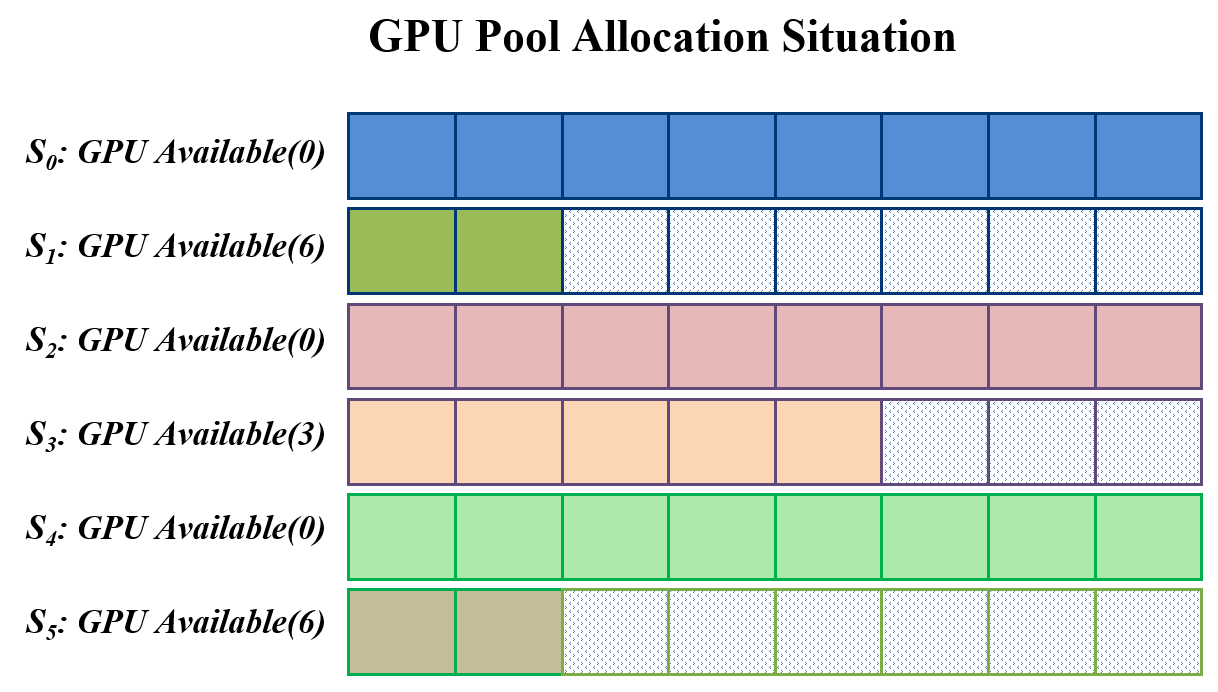
\includegraphics[width=\columnwidth]{Pic/Fig_01.png}}
\caption{스케줄링 전 GPU 서버 풀의 점유 상태 --- 각 서버에 일부 GPU만 남아 단편화된 모습.}
\label{fig:01}
\end{figure}

\begin{figure}[htb!]
\centerline{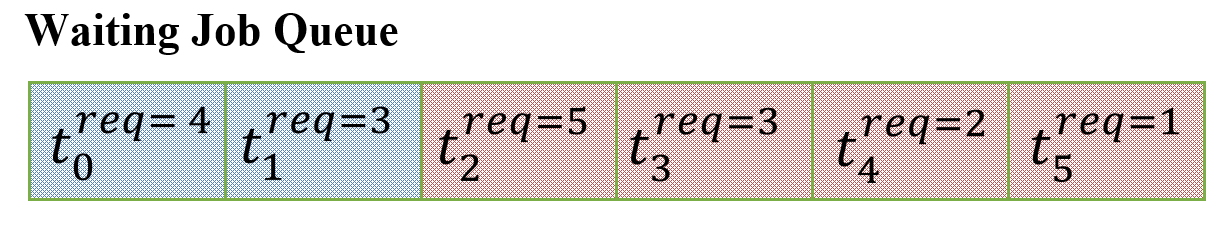
\includegraphics[width=\columnwidth]{Pic/Fig_02.png}}
\caption{동일 시점의 작업 대기 큐 --- 작업 $t_0$--$t_5$와 각 작업의 요청 GPU 수.}
\label{fig:02}
\end{figure}

그림 \ref{fig:01}과 그림 \ref{fig:02}는 각각 GPU 서버 풀과 작업 대기 큐의 상태를 보여준다. most-allocated 방식을 사용하는 스케줄러는 작업 $\textit{t}_{0}$과 $\textit{t}_{1}$을 할당할 수 있다. 그러나 $\textit{t}_{2}$는 다른 작업들이 완료되어 GPU 슬롯이 비워지기를 기다려야 하므로 스케줄링할 수 없다. 이는 작업 $\textit{t}_{3}$, $\textit{t}_{4}$, $\textit{t}_{5}$가 그 이후에야 스케줄링될 수 있음을 의미한다(그림 \ref{fig:03}).

그림 \ref{fig:03}에 나타난 것처럼, $\textit{t}_{3}$, $\textit{t}_{4}$, $\textit{t}_{5}$를 스케줄링하기에 충분한 GPU 슬롯이 있음에도 이 작업들은 $\textit{t}_{2}$ 때문에 스케줄링되지 못한다. 이것이 HOL 블로킹이다. 이는 앞서 할당된 작업들이 GPU 서버 풀을 단편화시키기 때문이다. GPU 서버 풀의 단편화는 운영 중 지속적으로 발생하며 간헐적으로만 해소된다. 최악의 경우는 모든 GPU 서버에 7장의 GPU가 남아 있는데 HOL 블로킹 작업이 8장을 요청하는 상황이다.

이 경우 GPU 서버 풀은 어떤 작업이 완료되기 전까지 낮은 GPU 할당률에 머무른다(그림 \ref{fig:03}). 다만 이 할당률 손실은 \textit{중간 부하}에서 두드러지는 증상이다. 작업이 끊임없이 제출되어 클러스터가 포화되는 \textit{과부하}에서는 빈 슬롯이 곧 다른 작업으로 채워져 할당률은 높게 유지되며(\S\ref{eval:main}에서 모든 정책이 약 99\%), 이때 HOL 블로킹의 비용은 할당률 손실이 아니라 막힌 작업들의 \textbf{큐 지연}과 \textbf{도착 순서 불공정}으로 전환된다. 어느 부하에서든 근본 병목은 단편화에서 비롯된 HOL 블로킹이며, 본 연구는 이를 큐 전처리로 완화한다.

\begin{figure}[htb!]
\centerline{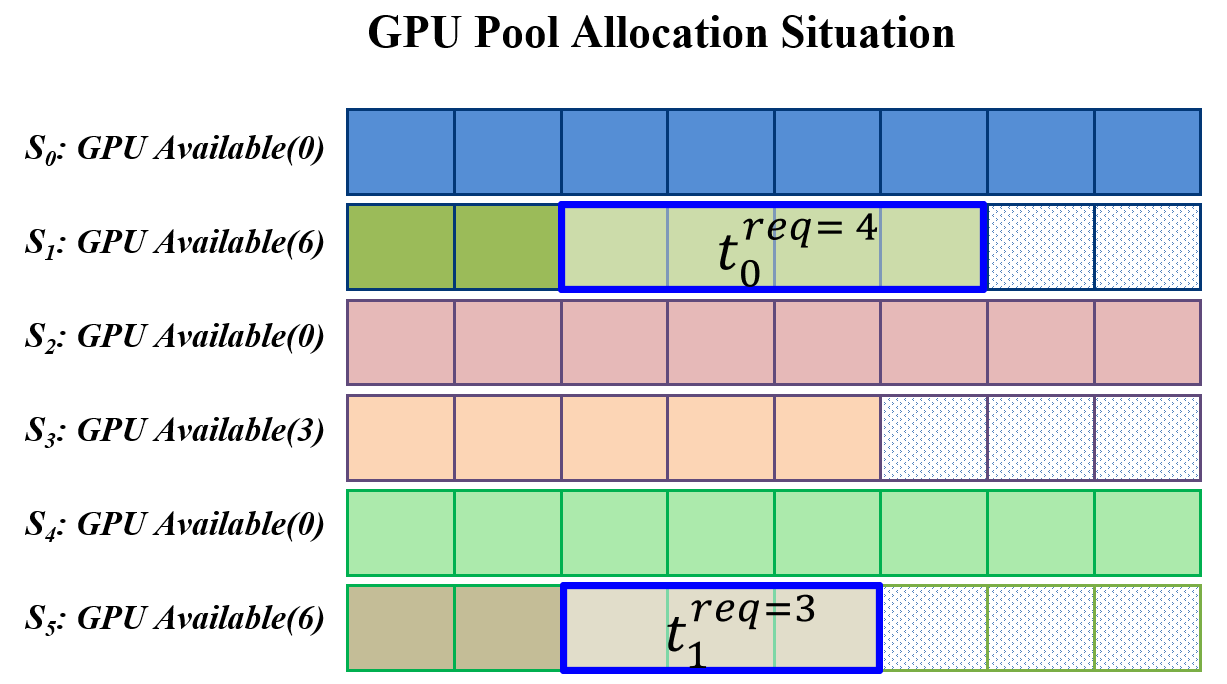
\includegraphics[width=\columnwidth]{Pic/Fig_03.png}}
\caption{most-allocated 스케줄링 후 --- 8 GPU를 요청하는 $t_2$의 HOL 블로킹으로 $t_3$--$t_5$가 함께 지연된 상태.}
\label{fig:03}
\end{figure}

이 HOL 블로킹은 정책 선택만으로 제거되지 않는다. 여러 스케줄링 정책을 동일 조건에서 비교하면, 중앙값 대기와 최악 대기(기아)는 서로 맞바꾸어지는(trade-off) 관계를 이룬다. 여러 정책을 동일 조건에서 비교하면 중앙값 대기와 순서 공정성·최악 꼬리가 일반적으로 맞바꿔지는 경향이 관찰되지만, 이는 법칙이 아니라 \textit{측정으로 확인할 경험적 경향}이다 --- 실제로 본 평가에서도 일부 셀은 두 축이 함께 개선된다(이종 512의 SAFA는 FIFO 대비 중앙값과 최악 꼬리를 모두 줄인다). 따라서 본질적 과제는 ``어느 균형점을 택할 것인가''와 ``그 점을 워크로드가 바뀔 때마다 재튜닝 없이 유지할 수 있는가''로 귀결되며, 이것이 SAFA의 설계 동기를 형성한다. 본 논문은 이 트레이드오프 구조를 \S\ref{eval:main}의 대규모 시뮬레이션에서 정량적으로 확인한다.


왜 이 단편화가 고전적 CPU 스케줄링의 기아와 \textit{질적으로} 다른지 짚어 둘 필요가 있다. 단일 자원(CPU 시간)을 다루는 고전 스케줄링에서 기아는 \textit{낮은 우선순위의 장기 미배치} 문제이며(동기화 현상인 priority inversion과는 별개 개념이다), 시분할(time-slicing)과 선점으로 굶은 작업에 언제든 한 조각의 CPU를 떼어 줄 수 있어 priority aging만으로 원리적으로 해소된다 --- 한 작업이 받는 자원은 연속적으로 분할 가능하다. 그러나 GPU 갱(gang) 스케줄링의 HOL 블로킹은 \textit{공간적·불가분(all-or-nothing) 자원 단편화}에서 비롯된다. 8-GPU 작업은 8장이 \textit{동시에·한 갱으로} 확보되어야만 실행되며(부분 실행 불가), 빈 GPU가 여러 서버에 7장씩 흩어져 있으면 총량이 충분해도 배치할 수 없다. 게다가 GPU 작업은 비선점이 사실상의 표준이다 --- 학습 작업의 체크포인트·재적재 비용이 크고(리젝 ②의 GPU 선점 비현실성과 일치), 본 환경도 전 정책 비선점이다. 따라서 굶은 큰 작업에 ``자원의 한 조각''을 떼어 주는 CPU식 완화가 불가능하며, 기아 해소는 오직 \textit{큐 순서}를 통해 ``그 작업이 들어갈 연속 슬롯이 비는 순간까지 후속 작업이 자리를 영구히 잠식하지 못하게 하는'' 방식으로만 가능하다. 정확히 하면, 불가분·비선점·공간 단편화의 결합 자체는 새롭지 않다 --- 공간 공유 병렬 작업 스케줄링(JSSPP 계보\cite{feitelson1996toward})의 창립 가정이고, Maui의 XFactor·대기시간 가중\cite{jackson2001maui}과 Slurm age factor가 바로 그 맥락에서 aging을 수십 년 운용해 왔다. 본 연구가 이 고전 맥락에 더하는 새 요소는 두 가지로 한정된다: \textit{노드 경계 패킹의 자리 적합($R$)을 aging에 결합}하는 것과, 그 계수를 \textit{큐 통계로 정규화해 무튜닝으로} 만드는 것(각각 \S\ref{eval:ablation:comp}·\S\ref{eval:ablation:grid}에서 성분 격리). SAFA가 선점이나 자원 분할 없이 큐 순서만으로 동작하도록 설계된 이유가 여기에 있다.

처리 시간이 알려진 유한 입력의 오프라인 스케줄링조차 NP-hard이며\cite{ullman1975np}, 완료 시간·도착 시점을 모르는 본 설정은 비예지 온라인 문제로서 경쟁비 하한이 별도로 존재한다\cite{motwani1994nonclairvoyant}. 따라서 이 문제는 스케줄링 알고리즘만으로는 완전히 해결될 수 없다. 더욱이 완료 시간·도착 시점이라는 \textit{미래 정보}는 본질적으로 예측 불가능하므로, 이를 추정해 HOL 블로킹을 \textit{예방}하려는 접근(작업 실행시간 추정, 성능 프로파일)은 추정 오차와 프로파일링 비용에 취약하다. 이에 본 연구는 스케줄링 알고리즘의 개선이나 미래 예측이 아니라, \textit{큐에 이미 드러난 정보} --- 각 작업의 대기 시간, 자원 요구량, 상대 나이 --- 만으로 단편화에서 비롯되는 HOL 블로킹을 \textit{사후}에 완화하는 것을 우선시한다. 그 결과 우리는 이 큐 관측 신호만으로 작업 대기 큐를 재정렬하는 큐 조정(queue adjustment) 메커니즘을 제시한다.

우리는 HOL 블로킹 해소 메커니즘의 분석과 신속한 반복 개발을 위해 작업 스케줄링용 자체(in-house) 시뮬레이션을 개발했다. 이 시뮬레이터는 작업 로그를 파싱하고 다양한 방식으로 스케줄링에 응답한다. 기존 메커니즘에 영향을 주지 않고 새로운 스케줄링 방법론을 추가할 수 있다. 이는 큐 조정이 작업 스케줄링 방식과 독립적으로 동작함을 의미한다.

\section{Resolving Head-of-Line Blocking in the Job Queue}\label{algo:intro}
우리는 작업 대기 큐의 HOL 블로킹을 해소하기 위한 기아 인지 공정 나이가중(Starvation-Aware Fair Aging) 알고리즘 SAFA를 제안한다. 용어를 정리해 두면, 본 논문의 ``gang''은 GPU 스케줄링 문헌의 관용대로 \textit{전부-아니면-전무로 동시 할당되는 고정 GPU 요청}을 가리키며, Feitelson--Rudolph 고전 분류\cite{feitelson1996toward}의 rigid job에 해당한다(조율된 시분할을 뜻하는 Ousterhout류 고전 gang scheduling\cite{ousterhout1982gang}과 구별). SAFA는 나이 가중 계수 $\alpha$로 트레이드오프를 제어하는데, 기본형은 $\alpha$를 고정하지만(SAFA(고정 $\alpha$)), 본 논문의 SAFA는 계수 튜닝을 제거해 $\alpha$를 관측된 큐 나이 통계로 정규화한다(무튜닝). SAFA는 배치 단계 앞에서 어드미션 순서를 결정하는 계층으로서 작업 대기 큐를 재정렬하여, 단편화에서 비롯되는 HOL 블로킹을 직접 완화한다. SAFA는 배치 정책의 종류·메커니즘과 무관하게 작동하며, 그 트레이드오프는 나이 가중치 계수 $\alpha$로 제어된다. SAFA는 이 $\alpha$마저 큐 나이 통계로 정규화하여 제거한다.
\subsection{Starvation-Aware Queue Adjustment}
본 연구가 제안하는 큐 조정은 사용하는 스케줄러의 종류나 방식과 무관하게, HOL 블로킹으로 인한 큐 지연을 줄이고 작업의 도착 순서 공정성을 지키는 것을 목표로 한다(처리량·할당률 자체를 높이는 것이 목표가 아니라, 동일 처리량 아래에서 대기를 공정하게 재분배한다). 이 알고리즘은 스케줄러 실행 전에 동작하여 작업 대기 큐를 재정렬함으로써, 스케줄러의 종류나 메커니즘과 무관하게 일관된 효과를 낸다.

HOL 블로킹은 GPU 서버 풀 운영 중 빈번히 발생하며 결국에는 해소되지만, 그 해소에 오랜 시간이 걸릴 수 있다. 중간 부하에서는 이 지연이 할당률을 떨어뜨리고, 과부하에서는 막힌 작업들의 큐 대기와 순서 불공정으로 누적된다. HOL 블로킹을 예방하는 스케줄링은 NP-hard 문제이며, HOL 블로킹이 언제 발생할지 예측하는 것은 거의 불가능하다. 현실 세계에서 GPU를 요청하는 작업의 유형과 요구 자원이 예측 불가능하기 때문이다. 따라서 HOL 블로킹을 예방하려는 스케줄링은 간접적인 접근에 머무른다. 본 알고리즘은 대기 큐에 있는 작업들의 우선순위를 직접 수정함으로써 막힘 문제를 완화한다. 우리는 이러한 수정이 낳는 트레이드오프 또한 특정 계수들을 사용해 고려한다. 큐를 조정하면 막힘에 가로막힌 작업들이 스케줄링될 수 있게 되지만, 최악의 경우 막힘을 유발하는 가장 큰 작업 자체는 계속 자리가 비기를 기다린다. 따라서 본 알고리즘이 방지하는 것은 \textit{큐가 한 작업에 무한정 막혀 후속 작업들이 영구히 적체되는 상태}이며, 개별 대형 작업의 완료를 보장하는 것은 아니다(이 정직한 범위는 \S\ref{SAFA}와 \S\ref{eval:main}에서 명확히 한다). 우선순위를 임의로 조정하면 새로운 공정성 문제가 발생할 수 있으므로, 본 알고리즘은 나이 가중으로 그 트레이드오프를 제어한다.

$P^*$를 작업 $t_0^*$, $t_1^*$, $t_2^*$, \dots, $t_n^*$의 조정된 우선순위 값이라 하자. $P^*$는 스케줄링이 시작되기 전에 계산되어 재부여된다. 스케줄러는 수정된 작업 우선순위를 사용한다. 조정된 작업 우선순위 $P^*$는 다음과 같이 정의된다:

\begin{equation}
P^* = P + \alpha A \times R
\label{eq:01}
\vspace{1em}
\end{equation}

첫 번째 항 $P$는 작업 $t_0$, $t_1$, \dots, $t_n$의 원래 우선순위를 나타내며, 여기서 $n$은 서버 수의 3배다. 구체적으로 우선순위는 $p_0$ = 1, $p_1$ = 0.5, $p_2$ = 0.25와 같이 정의되어 이후 우선순위가 절반씩 감소하며, 값이 클수록 우선순위가 높다. 두 번째 항은 기아 지수(starvation index)를 나타내는 변수 $\alpha A \times R$로 구성된다. 여기서 $\alpha$는 기아 지수가 중요성을 얻는 속도를 결정하는 계수다. 예컨대 대기 큐의 두 번째 작업의 우선순위가 6시간 안에 역전되도록 하려면, $R$을 1로 가정할 때 $\alpha$는 최소 0.013889로 설정되어야 한다. 수치로 보면 $P_1$이 0.5일 때 $0.013889 \times 36 \times 1 = 0.500004$가 계산되어 갱신된 우선순위는 1.000004가 되고, 이는 $P_0$ 값 1을 넘어서므로 순위 추월이 일어난다. (이 예시는 직관을 위해 선두 작업 자신의 나이 보너스를 무시한 단순화다 --- 선두에도 $\alpha A_0 R_0$가 붙으므로 실제 역전은 두 작업의 $A\cdot R$ 곱 차이가 base 우선순위 차이를 넘을 때, 즉 자리 적합 $R$의 차등이 있을 때 일어난다. \S\ref{eval:ablation:comp}에서 $R$이 균일하면 역전이 전혀 일어나지 않음을 측정으로 보인다.) 이때 $A$는 작업의 나이(age)로 10분마다 1씩 증가하며, $R$은 자원 적합도 지수(resource suitability index)다. $A$는 작업이 스케줄링되면 초기화된다. $R$ 값은 요구 가속기 수가 가용 수 이내이면 1이고, 가용을 초과하는 부족분 하나마다 $0.1$씩 감소한다. 주목할 점은 \eqref{eq:01}의 세 입력이 \textit{모두 큐에서 직접 관측된다}는 것이다 --- $P$는 큐 위치, $A$는 대기 시간(나이), $R$은 요청 가속기 수 대 가용 수의 적합도. 즉 SAFA는 작업 실행시간 추정이나 잡별 성능 프로파일 없이, 큐와 서버의 현재 상태만으로 우선순위를 재계산한다. 이 형태는 우선순위가 대기 시간에 선형 비례해 자라는 Kleinrock의 time-dependent(delay-dependent) priority 규율\cite{kleinrock1976queueing}의 직계로, 본 기여는 그 고전 골격에 불가분 갱 자원 적합도 $R$을 결합하고(\S\ref{sec:coeff}) 계수를 큐 통계로 정규화한(\S\ref{SAFA}) 데 있다. Algorithm \ref{alg:adjust_wait_queue}는 \eqref{eq:01}을 사용한 기아 방지 알고리즘의 구현을 보여준다.

\begin{algorithm}
\caption{Starvation-Aware Queue Adjustment}\label{alg:adjust_wait_queue}
\textbf{Input:} \\
\hspace*{4mm} Server count : \( \boldsymbol{n} \), Wait queue length : \( \boldsymbol{l_{wq}} \) \\
\hspace*{4mm} Servers :\( \boldsymbol{S_i} \in \{S_0, S_1, \ldots, S_{n-1}\} \), \\ 
\hspace*{4mm} Accelerator count in $S_i$: \( \boldsymbol{M_i} \in \{M_0, M_1, \ldots, M_{n-1}\} \), \\ 
\hspace*{4mm} Resource suitability index : \( \boldsymbol{R_i} = 0, \forall i \in \{1, 2, \ldots, 8\} \), \\
\hspace*{4mm} Wait Queue : \( \boldsymbol{WQ_i} \in \{WQ_0, WQ_1, \ldots, WQ_{l-1}\} \), \\
\hspace*{4mm} Task in $WQ$ : \( \boldsymbol{t_i} \in \{t_0, t_1, \ldots, t_{l-1}\} \), \\
\hspace*{4mm} Accelerator request of $t_i$ : \( \boldsymbol{a_{t_i}} \), \\
\hspace*{4mm} Idle accelerator count in $S_i$ : \( \boldsymbol{f_{S_i}} \) \\
\hspace*{4mm} Wait Age : \( \boldsymbol{A_i} \in \{A_0, A_1, \ldots, A_{l-1}\} \)
\begin{flushleft}
\textbf{Procedure:} Updated wait queues
\end{flushleft}
\begin{algorithmic}[1]
\STATE $R \gets 0$
\STATE {}
\FOR{ $i \gets 0$ to $n-1$}
    \FOR{$j \gets 1$ to $M_i$}
        \IF{$j > f_{S_i}$}
            \STATE $R_j \gets \max\{R_j,\ 1 - ( j - f_{S_i} ) \times 0.1\}$ \COMMENT{요청 $j$가 가용 $f_{S_i}$를 초과: 부족분당 0.1 감소}
        \ELSE
            \STATE $R_j \gets 1$ \COMMENT{가용 충분: 완전 적합}
        \ENDIF
    \ENDFOR
\ENDFOR
\STATE {}
\FOR{ $i \gets 0$ to $l_{wq}-1$}
    \STATE $P_i \gets 1/2^i$
    \STATE $P_i^* \gets P_i + \alpha A_i \times R_{a_{t_i}}$
\ENDFOR
\STATE {}
\STATE $(P_{i_{\max}}^*, i_{\max}) \gets \max(P^*)$
\IF{$i_{\max} \neq 0$}
    \STATE $WQ \gets [\,t_{i_{\max}},\ t_0,\ \ldots,\ t_{i_{\max}-1},\ t_{i_{\max}+1},\ \ldots,\ t_{l-1}\,]$ \COMMENT{단일 승급: $P^*$ 최대 작업만 맨 앞으로, 사이 작업은 한 칸씩 뒤로}
\ENDIF
\end{algorithmic}
\end{algorithm}

SAFA는 스케줄러와 독립적으로 동작하며, 일정 주기로 동작하는 스케줄러보다 먼저 실행된다. 이는 동작 결정에 작업 대기 큐와 서버 풀 내 현재 작업 할당 상태만을 사용하므로, 코어 스케줄러의 종류나 메커니즘과 무관하게 작업 대기 큐를 최적화하는 전처리기로 기능한다. 다만 본 연구는 작업 대기 큐를 직접 관리하므로, 큐에 대한 스케줄링을 자체적으로 수행하거나 누적 지표·컨텍스트에 의존하는 스케줄러는 대상으로 하지 않는다.

\textbf{복잡도와 최적성에 대하여.} Algorithm \ref{alg:adjust_wait_queue}는 한 패스에서 큐를 한 번 훑어 $P^*$가 최대인 작업 \textit{하나}만 큐 앞으로 올리므로 큐 길이 $l_{wq}$에 대해 $O(l_{wq})$, 즉 단일 승급 $O(n)$이다(자원 적합도 $R$ 계산은 서버 수에 선형). 이 경량성은 의도된 설계 선택의 결과다 --- 전 순열 공간($l_{wq}!$)을 탐색하는 전역 최적 재배열은 조합적으로 비현실적이므로, 우리는 최적해를 추구하지 않고 ``매 패스 가장 굶은 작업 하나를 승급''하는 탐욕적 휴리스틱으로 이를 회피한다. 따라서 SAFA는 어떤 정적 목적 함수에 대한 \textit{근사 비(approximation ratio) 보장이나 최적성 경계를 제공하지 않으며}, 그 효용은 분석적 경계가 아니라 \S\ref{eval:main}의 정책 간 직접 측정으로만 입증된다 --- 이는 $O(n)$ 무튜닝 경량성과 맞바꾼, 본 설계가 명시적으로 받아들인 한계다.

\section{Optimization of Coefficient $\alpha$}\label{sec:coeff}
기아 방지 알고리즘은 트레이드오프 제어를 위해 나이 가중치 계수 $\alpha$를 사용한다. 이 절은 다음 순서로 전개된다: 먼저 $\alpha$가 제어하는 트레이드오프를 정량화하고 그 최적값을 정의한다. 이어 최적 $\alpha$가 워크로드 특성에 따라 크게 달라져 고정 계수에는 단일 최적값이 없음을 보이고, 끝으로 이 한계를 제거하기 위해 계수 결정을 큐잉 이론에 위임한 무튜닝 SAFA를 유도한다.

\subsection{Trade-off analysis and definition of related metrics}
$\alpha$는 HOL 블로킹 제거에 도움을 주지만, 값이 지나치게 크면 막혀 있던 작업이 다른 작업을 과도하게 추월하여 새로운 불공정을 낳을 수 있다. 적절한 $\alpha$를 정하려면 이 트레이드오프를 정량화해야 한다. 이에 각 작업의 누적 대기 시간을 요청 가속기 수로 묶어 트레이드오프로 산정하며, 이를 누적 평균 거리(accumulated average distance, AAD)로 정의한다.
\begin{equation}
AAD = \sum_{k=1}^8 \frac{(WT'_k - WT_k)}{2^{8-k}}
\tag{2}
\label{eq:07}
\end{equation}

식 \eqref{eq:07}은 $\alpha$ 적용 전후 대기 시간의 가중 평균 차이를 측정한다. 요청 가속기 수 $k$의 작업 클래스를 $C_k$라 할 때, $WT_k=\sum_{j\in C_k} w_j$는 적용 전 대기 시간 합, $WT'_k$는 적용 후 합이다. 가중 $1/2^{8-k}$는 큰 작업 클래스에 지수적 비중을 두려는 설계 선택이나, $WT_k$가 클래스 \textit{합}이라 클래스 크기 비가 이 가중을 부분 상쇄할 수 있음(Philly는 1-GPU가 다수)도 함께 명시한다 --- 어느 쪽이든, 이 가중의 임의성이 \S\ref{SAFA}의 무튜닝 동기 중 하나다(아래 참조). 한편 클래스별 \textit{최악} 대기의 변화를 같은 가중으로 누적한 누적 최대 거리(accumulated maximum distance, AMD)는 식 \eqref{eq:08}로 정의된다:

\begin{equation}
AMD = \sum_{k=1}^8 \frac{\max\limits_{j\in C_k} w'_j \;-\; \max\limits_{j\in C_k} w_j}{2^{8-k}},
\tag{3}
\label{eq:08}
\vspace{1em}
\end{equation}
여기서 $w_j$/$w'_j$는 적용 전/후 작업 $j$의 대기 시간이다($C_k=\emptyset$이면 해당 항은 0). 식 \eqref{eq:07}--\eqref{eq:08}과 그 min--max 정규화 합(식 \eqref{eq:09})은 $\alpha$ \textit{탐색의 목적함수}일 뿐 본 논문의 평가 지표가 아니며, 가중·정규화 선택에 따라 최적 $\alpha$ 수치가 달라질 수 있다는 점이 바로 ``단일 고정 $\alpha$는 워크로드·목적함수에 민감하다''는 \S\ref{coeff:limit}의 논지를 한 겹 더 뒷받침한다.

이 지표들의 계산은 작업 대기 시간의 평균 편차와 최대 편차를 모두 고려하여, 스케줄링의 공정성을 강제하고 기아나 과도한 대기로 인한 성능 저하를 방지한다.

\subsection{Objective function}
$\alpha$는 wall time, AAD, AMD를 최소화하도록 조정된다. 최적값을 결정하기 위해 $\alpha$ 값 범위(0.01--1.99, 0.01 간격)에 대해 탐색을 수행하고, 각 값에서 세 지표를 계산한다. 지표 간 공정한 비교를 위해 세 지표 모두 min--max 스케일러로 정규화한 뒤 합산하여 목적 함수를 정의하며, 이를 최소화하는 $\alpha$를 선택한다.

\begin{equation}
Obj_i^{sfa} = walltime_i^{norm} + AAD_i^{norm} + AMD_i^{norm}
\tag{4}
\label{eq:09}
\vspace{1em}
\end{equation}

\subsection{Limitation of a fixed coefficient}\label{coeff:limit}
고정 $\alpha$ 방식의 근본 한계는 \textit{최적 $\alpha$에 단일 값이 없다}는 것이다. 이를 확인하기 위해, 8가지 작업 분포(정규·지수·로그 정규·감마·베타·Weibull minimum·균등·푸아송)로 각 1,000개의 작업을 합성하고, 이산 시간 C++ 시뮬레이터로 $\alpha$를 0.01--1.99(0.01 간격) 범위에서 탐색하여 \eqref{eq:09}의 목적 함수를 최소화하는 분포별 최적값을 구했다. 그림 \ref{fig:motivation}이 보이듯 최적 $\alpha$는 분포에 따라 0.22(감마·푸아송)에서 1.63(로그 정규)까지 약 7배 달라진다 --- 모든 워크로드를 만족시키는 단일 $\alpha$는 존재하지 않는다. 따라서 한 번 고정한 $\alpha$는 특정 워크로드에 대한 타협일 뿐이며, 워크로드가 바뀔 때마다 그리드 탐색을 다시 수행해야 한다. 이 한계의 뿌리는 ``고정된 절대 시간 단위''다 --- 나이 가중치가 절대 초 단위로 고정되어 있어, 작업 분포나 대기 시간 스케일이 달라지면 의도한 균형점을 벗어난다. 이것이 \ref{SAFA}절의 무튜닝 SAFA를 설계한 직접적 동기다.

\begin{figure}[htb!]
\centerline{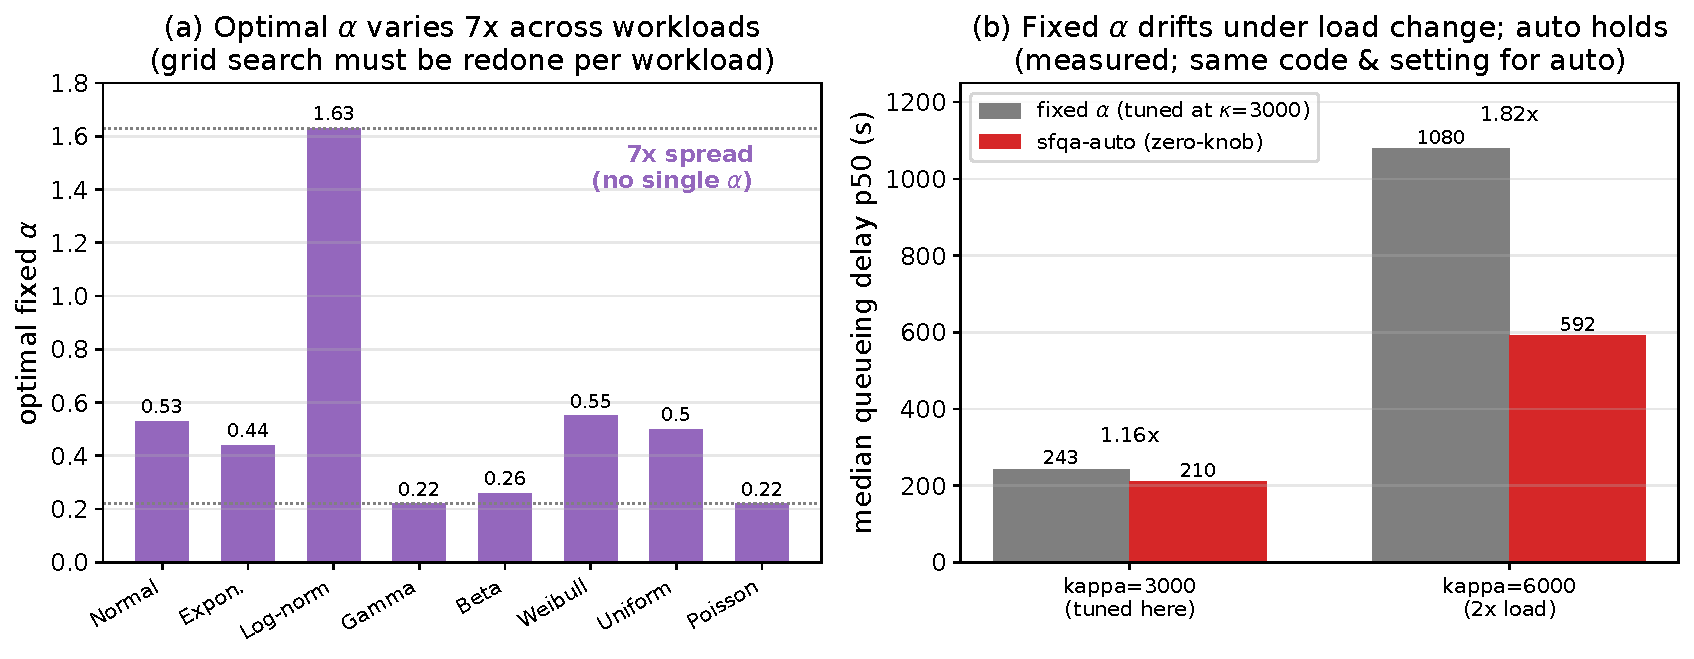
\includegraphics[width=\columnwidth]{Pic/Fig_18.pdf}}
\caption{8개 작업 분포에서의 최적 고정 $\alpha$ --- 약 7배(0.22--1.63) 변동하여 모든 워크로드를 만족하는 단일 값이 없다.}
\label{fig:motivation}
\end{figure}

\subsection{Zero-knob, Scale-Normalized SAFA}\label{SAFA}
\ref{coeff:limit}절에서 본 고정 $\alpha$의 한계를 없애기 위해, 우리는 고정-$\alpha$ SAFA의 식과 동작을 그대로 계승하되 계수 $\alpha$를 관측 가능한 큐 통계만으로 매 스케줄링 시점에 동적으로 결정해 튜닝 노브를 제거한다(이것이 본 논문의 SAFA다). 실제 평가된 규칙은 다음과 같다. SAFA의 우선순위 구조를 그대로 두고, 각 대기 작업 $j$에 대해
\begin{equation}
P^*_j = \frac{1}{\text{base}^{\,pos_j}} + \alpha_{\text{eff}}\cdot \tilde A_j \cdot R_j
\tag{5}
\label{eq:auto-pstar}
\end{equation}
를 계산한 뒤, $P^*$가 최대인 작업 \emph{하나만} 큐 맨 앞으로 올린다(단일 승급, Algorithm \ref{alg:adjust_wait_queue}와 동일 구조). $pos_j$는 도착순 큐 위치, $\text{base}=2.0$(기본), $R_j$는 식 \eqref{eq:01}의 자원 적합도 지수다.

설계의 출발 직관은 PS-공정 속도저하 $\sigma^*=1/(1-\rho)$\cite{wierman2003classifying} --- ``현재 부하에서 이상적 공평 분배(PS)였다면 겪었을 속도 저하까지는 정상'' --- 였으나, 이 양은 SAFA의 운영 규칙 어디에도 입력되지 않으며($\rho$ 자체를 계산하지 않는다), 점유율 기반 $\rho$ 추정은 본 평가의 과포화(할당률 99--100\%)에서 1로 포화해 의미를 잃는다. 따라서 우리는 $\sigma^*$를 수식이 아닌 \textit{출발점이 된 직관}으로만 남기고, 실제 메커니즘을 그 자체로 정확히 서술한다: SAFA의 적응은 부하 적응이 아니라 \textbf{나이-스케일 정규화}(scale normalization)다 --- 계수를 큐의 \textit{상대 나이 스케일}로 정규화해, 워크로드의 시간 단위가 무엇이든 승급 문턱이 \textit{큐의 나이 통계 그 자체}($A_{\text{ref}}$·$A_{\max}$의 무차원 결합)로 정해지는 \textit{단위-소거 규칙}을 유지하는 것이다(정확한 문턱은 식 \eqref{eq:auto-alpha} 아래 부등식 참조 --- $A_{\max}$와 $A_{\text{ref}}$가 함께 들어가는 큐-통계 결합이다).

이 규칙의 핵심은 계수 $\alpha_{\text{eff}}$를 외부 상수 없이 큐 통계만으로 동적으로 정하는 것이다:
\begin{equation}
\alpha_{\text{eff}} = \frac{g}{A_{\text{ref}}\,R_{\min}},\qquad g=\min\!\Big(1,\;\frac{A_{\max}}{A_{\text{ref}}}\Big),
\tag{6}
\label{eq:auto-alpha}
\end{equation}
여기서 큐 상대 나이 $\tilde A_j = A_j - \min_k A_k$, 동적 나이 스케일 $A_{\text{ref}} = \max(1,\,\text{mean}(\tilde A))$, $A_{\max}=\max_k \tilde A_k$, 그리고 자리 적합이 가장 나쁜(=가장 큰) 작업의 적합도 $R_{\min}=\max(0.1,\,\min_k R_k)$다(8-슬롯 노드에서는 식 \eqref{eq:01}의 $R\ge0.2$라 바닥 0.1은 도달하지 않는 방어 상수다). 항 $g$의 역할은 정직하게 한정한다: $A_{\max}\ge\text{mean}(\tilde A)$가 항상 성립하므로 $g$는 상대 나이가 존재하는 모든 큐에서 1로 포화하며, $g<1$(즉 $g=0$)은 모든 후보의 상대 나이가 0인 자명한 경우 --- 그때는 나이 보너스 자체가 0이라 $g$가 결과를 바꾸지 않는다 --- 뿐이다(정수 도착-카운터 나이 기준 --- Philly 512 이종 전체 재생 122,952 패스에서 $g<1$은 1.65\%, 전부 이 자명 사례; wall-clock 나이에서는 $g\in(0,1)$이 가능하다). 따라서 \eqref{eq:auto-alpha}의 \textbf{실효 형태는 $\alpha_{\text{eff}}=1/(A_{\text{ref}}R_{\min})$}이고, $g$는 부하 게이트가 아니라 경계 사례를 0으로 처리하는 가드일 뿐이다 --- 우리는 이를 ``기아 압력 게이트''로 표현하지 않는다. $R_{\min}$ 분모의 역할도 정확히 한정한다: 시간-단위 소거는 $A_{\text{ref}}$만으로 완결되므로 $R_{\min}$ 나눗셈은 정규화가 아니라 승급 강도를 키우는 \textit{이득(gain) 항}이며, 큐에 큰 작업이 들어오고 나갈 때 예산이 계단형으로 변하는 거칠음을 가진다. 단독 ablation으로 제거하면(512 이종) $p1$ 75.2·$q_{p50}$ 2.31M초로 FIFO 쪽 frontier 점으로 이동한다 --- 즉 이 항 역시 $R$ 감쇠처럼 효율--공정 균형점의 위치를 정하는 설계 상수이고, 세 트레이스에서 같은 형태로 일관 작동한다는 것이 채택 근거다. 큐 상대 나이를 쓰므로 배치로 큐 멤버가 바뀌면 $\min_k A_k$가 갱신되어 남은 작업의 나이가 자동 재기준되고, 과포화에서 절대 나이가 무한히 누적돼도 $\tilde A$는 현재 큐의 spread로 제한되어 안정적이다. 승급 조건을 정확히 쓰면 다음과 같다: 선두에도 나이 보너스가 붙으므로($\tilde A_{\text{head}}=A_{\max}$가 큐 최대), 작업 $j$의 승급은 $\alpha_{\text{eff}}(\tilde A_j R_j - A_{\max}R_{\text{head}}) > 1 - \text{base}^{-pos_j}$일 때 일어난다 --- 즉 \textbf{나이 열세를 자리 적합 우위($R_j>R_{\text{head}}$)가 상쇄할 때만} 승급되며, $R$이 균일하면 선두가 항상 이긴다(\S\ref{eval:ablation:comp}의 $R\equiv1$ FIFO 동치와 정합). $1/(A_{\text{ref}}R_{\min})$ 정규화는 이 비교를 큐의 나이 스케일과 무관한 무차원 비교로 만든다. 여기서 한 가지를 명확히 해 둔다. SAFA가 올리는 것은 \emph{자리가 맞는(R이 큰) 굶은 작업}이며, 큐 선두를 막는 HOL 주범인 가장 큰 작업 자신은 $R_{\min}$이라 나이 보너스가 가장 약해 스스로 승급되지 않는다. 따라서 SAFA가 제거하는 대상은 \emph{큐 수준의 HOL 정체(시스템 처리량 손실)}이며, 막힘을 유발하는 가장 큰 작업의 진행은 그에 맞는 자리가 비기를 기다린다. 승급 이벤트 감사(Philly 512 이종, 122,952패스)가 이 구도를 정량 확인한다: 승급은 패스의 87.9\%에서 발화하고, 승급된 작업의 87\%가 1-GPU(평균 가용 2.1슬롯)다 --- 즉 \textit{직접 승급의 수혜자는 빈 틈에 맞는 소형 작업}이고, 큰 작업이 얻는 것은 승급이 아니라 \textbf{선두 보존}(blocking 규율이 선두의 자리 순번을 지켜줌)이다. ``큰 작업 보호''를 승급 메커니즘에 귀속하지 않도록 이 구분을 명시해 둔다. 이런 의미에서 ``starvation-free''는 큐가 큰 작업 하나에 무한정 막히는 상태를 방지한다는 뜻이지, 개별 대형 작업의 완료를 보장하는 것은 아니다(대형 작업의 기아를 SJF 등과 정량 비교하는 별도 분석은 \S\ref{eval:main}에서 다룬다). 모든 양은 측정값에서 계산되며 작업 duration은 전혀 쓰지 않으므로(BSLD·SJF·2계층 순서 모두 없음), 우리가 제거한 것은 \emph{워크로드에 가장 민감한 단일 노브 $\alpha$}다. 나머지 내부 상수의 성격은 둘로 갈린다(주 엔진 p1 기준 측정, \S\ref{eval:robust:sens}): 밑 $\text{base}$는 1.5--4.0에서 p1 50--51.5로 \textbf{둔감}하고, $R$ 감쇠(기본 0.1)는 0.05--0.2에서 p1 50--98을 움직이는 \textbf{트레이드오프 위치 상수}다 --- 단 $\alpha$·$w$와 결정적으로 다른 점은, 같은 감쇠 0.1이 세 트레이스(Philly·Helios·Alibaba) 전부에서 재튜닝 없이 일관된 균형점을 준다는 것이다(워크로드-민감 노브가 아니라 운영자의 효율--공정 선호를 한 번 표현하는 설계 상수). 또한 SAFA는 고정형의 트리거 임계 $\beta$ 없이 \emph{항상} 발동하므로(상대 나이가 없는 큐에서는 보너스가 0이라 자연히 무개입 --- 별도 임계가 필요 없다), 제거되는 노브가 하나 더 늘어난다.

SAFA의 단일 승급 절차는 Algorithm \ref{alg:auto}에 정리한다. 기아 완화의 구동원을 정확히 명시한다: 주 평가 엔진의 나이는 도착 카운터이므로(\S\ref{eval:sim}) 완화는 \textit{시간}이 아니라 \textbf{후속 도착과 배치 사건에 구동}된다 --- 자리가 맞는 굶은 작업의 $\tilde A_j$는 새 작업이 도착할 때마다 커지고, 앞 작업이 배치로 빠지면 $\min_k A_k$ 재기준으로 상대 나이 구도가 갱신된다. 다만 이 압력의 동역학을 정직하게 쓰면: 정규화 분모 $A_{\text{ref}}$도 후속 도착과 함께 자라므로 승급 압력은 무한히 커지는 것이 아니라 $R$ 차등에 비례하는 수준으로 \textbf{포화}하며, $R$ 차등이 작은 작업은 끝내 승급되지 못할 수 있다 --- 즉 이것은 유계 보장이 아니라 \textit{$R$-차등 구동의 기아 완화}이고, 그 실효는 \S\ref{eval:main}의 과부하 측정으로 확인한다. 도착이 완전히 멈춘 큐에서는 순서가 더 바뀌지 않지만, 그 상태는 잔여 작업이 현재 순서대로 소진되는 무해한 구간이다. 이는 절대 보장이 아니라 $R$ 차등이 있는 작업의 추월 노출을 줄이는 완화이며($R_j\le R_{\text{head}}$인 작업은 승급 경로가 없다 --- 위 포화 논의), SAFA의 정체성은 ``나이로 기아를 막는다''가 아니라 ``나이-정규화된 자리 적합으로 정체를 절단한다''로 정확히 읽어야 한다. 이 무튜닝 적응의 대가는 작은 중앙값 양보이며, 그 대신 부하·이질성 전반에서 일관되게 높은 공정성을 얻는다는 점을 \S\ref{eval:main}에서 정량적으로 보인다.

\begin{algorithm}[htb!]
\caption{Zero-knob, Scale-Normalized SAFA}
\label{alg:auto}
\begin{algorithmic}[1]
\STATE \textbf{입력:} 대기 큐 $Q$(도착순), 작업별 나이 $A$
\IF{$Q=\emptyset$}
  \RETURN $Q$ \COMMENT{빈 큐}
\ENDIF
\STATE $\tilde A_j \gets A_j - \min_k A_k$ \COMMENT{큐 상대 나이(자동 재기준)}
\STATE $A_{\text{ref}} \gets \max(1,\,\text{mean}(\tilde A))$;~ $A_{\max} \gets \max_k \tilde A_k$
\STATE $R_{\min} \gets \max(0.1,\,\min_k R_k)$ \COMMENT{최악 자리적합}
\STATE $g \gets \min(1,\,A_{\max}/A_{\text{ref}})$ \COMMENT{경계 가드(본문 참조 --- 상대 나이 존재 시 항상 1)}
\STATE $\alpha_{\text{eff}} \gets g/(A_{\text{ref}}\,R_{\min})$
\FOR{각 $j \in Q$}
  \STATE $P^*_j \gets 1/\text{base}^{\,pos_j} + \alpha_{\text{eff}}\cdot \tilde A_j \cdot R_j$
\ENDFOR
\STATE $m \gets \arg\max_j P^*_j$
\IF{$m = 0$}
  \RETURN $Q$ \COMMENT{이미 선두}
\ELSE
  \RETURN $j_m$를 맨 앞으로 올린 $Q$ \COMMENT{단일 승급}
\ENDIF
\end{algorithmic}
\end{algorithm}

계수 $\alpha$를 제거한 뒤 SAFA에 남는 소수의 내부 상수가 또 다른 숨은 노브가 아님을 보이기 위해, 별도의 1차원 민감도 분석을 수행했다. 그림 \ref{fig:sensitivity}는 C++ 시뮬레이터로 12개 구성을 스윕한 결과를 보여준다 --- 자원 적합도 페널티 $R$(0.05--0.3)과 우선순위 밑 $P$(1.5--4)는 makespan 변동이 $\pm$2\% 이내로 둔감했고, 큐 재정렬 창 $m$만 $m$=1에서 +8.9\%로 민감했으며 $m\ge 2$에서는 1.4\% 이내였다(본 연구는 안전값 $m$=3 채택). 즉 이 상수들은 임의로 선택된 값이 아니라 넓은 범위에서 안정적이며, 유일하게 의미 있는 설계 선택($m\ge 2$)도 명확한 근거를 갖는다.

\paragraph{고전 aging과의 관계 --- 무엇이 새로운가}
나이에 따라 우선순위를 올리는 발상 자체는 새롭지 않다. 1990년대 운영체제의 priority aging, Linux CFS의 가상 실행시간(vruntime) 균등화, GPU 스케줄링의 Tiresias\cite{gu2019tiresias}(누적 서비스가 적은 작업 우선)는 모두 ``오래 기다리거나 덜 받은 작업을 끌어올린다''는 같은 계보에 속하며, 프로덕션 측에서는 Slurm의 multifactor 우선순위(2009년 도입)가 age factor(\texttt{PriorityMaxAge}에서 포화하는 대기 가중)를 운용해 온 가장 가까운 실전 선행이다. 본 연구의 기여는 \textit{aging이라는 메커니즘}이 아니라 \textit{그 가중을 무엇으로 정하는가}에 있으며, 세 가지 점에서 고전 aging과 갈린다. 첫째, \textbf{불가분 갱 자원에 대한 $R$ 결합}이다. CFS·Tiresias의 aging은 분할 가능한 단일 자원(CPU 시간·GPU-시간)을 전제하여 ``더 오래 기다린 작업''을 무조건 끌어올리지만, SAFA의 나이 보너스는 자원 적합도 $R_j$와 곱해져 \textit{지금 비는 자리에 맞는} 굶은 작업만 승급한다(\eqref{eq:auto-pstar}). 그 결과 HOL 주범인 가장 큰 작업($R_{\min}$)은 스스로 올라오지 않아, \S\ref{algo:intro}에서 논한 공간적·불가분 단편화에 aging을 정합시킨다 --- 이는 분할 가능 자원을 전제한 고전 aging에는 없는 결합이며, 단일 승급 구조에서 이 결합을 끄면($R\equiv1$) SAFA가 세 구성 모두에서 FIFO와 \textit{동치로 퇴화}함을, 그리고 전체 정렬형 aging은 발화하되 워크로드-민감 가중 노브를 요구함을 성분 ablation(\S\ref{eval:ablation:comp})이 보인다. 둘째, \textbf{절대 시간이 아닌 상대 나이}다. 고전 aging(Slurm age factor 포함)은 절대 대기 시간(초·tick)에 고정 계수를 곱하므로 워크로드의 시간 스케일이 바뀌면 재튜닝이 필요하다(\S\ref{sec:coeff}에서 해당 탐색 목적함수 기준 최적 $\alpha$가 분포별 7배 차이로 실증 --- 단 주 엔진에서는 잘 고른 단일 미세값도 세 트레이스에서 생존하므로(\S\ref{eval:ablation:grid}), 무튜닝의 가치는 ``단일값의 부재''가 아니라 \textit{탐색 없는 일관 균형점}이다). SAFA는 큐 상대 나이 $\tilde A_j$와 동적 스케일 $A_{\text{ref}}$로 정규화하여 시간 단위를 소거한다. 셋째, \textbf{큐-구동 무차원 가중}이다. Tiresias의 우선순위 키나 CFS의 vruntime은 절대 단위(누적 서비스 시간)에 고정 스케일로 작동한다. SAFA의 $\alpha_{\text{eff}}=1/(A_{\text{ref}}R_{\min})$는 현재 큐의 상대 나이 스케일 그 자체에서 유도되는 무차원 규칙이라, 정체가 쌓여 큐의 나이 spread가 형성될 때 그 spread를 기준으로 승급 문턱이 정해지고, spread가 없으면 보너스가 0이라 자연히 무개입이다. 요컨대 ``자동화''의 순효과 --- 단일 고정 $\alpha$ SAFA(고정 $\alpha$) 대비 무튜닝 SAFA의 이득 --- 를 같은 큐 전처리 골격 안에서 격리하는 정량 ablation은 \S\ref{eval:ablation}(표 \ref{tab:ablation})에서 제시한다. 나아가 구성별 그리드 탐색으로 얻은 \textit{워크로드별 최적} $\alpha$와의 비교(표 \ref{tab:ablation-grid})에서, \textbf{고정 $\alpha$ 역시 절대 나이 스케일에 절벽형으로 결합된 보간 노브이며, 무튜닝은 그 노브 없이 효율--공정성 균형점에 도달함}을 보인다.

\begin{figure*}[htb!]
\centerline{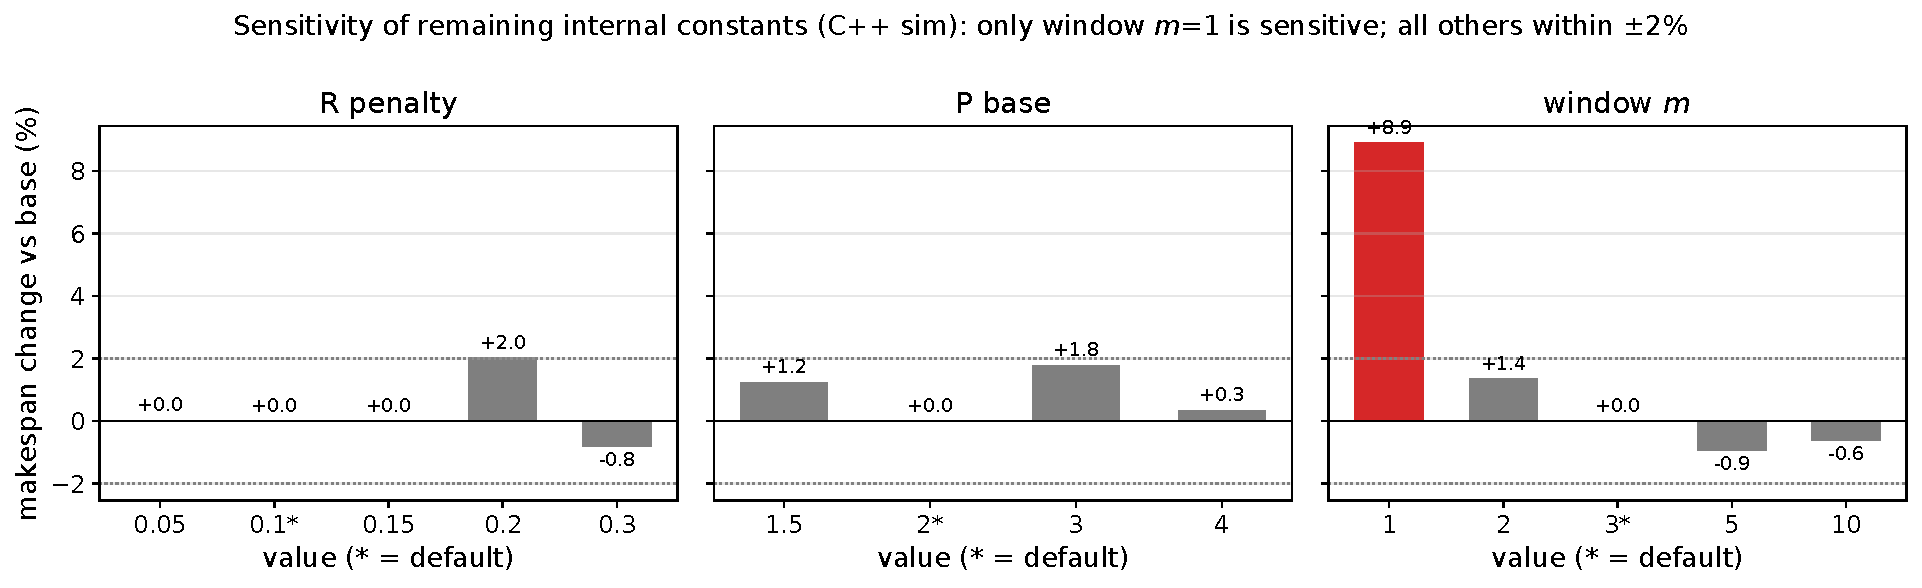
\includegraphics[width=\textwidth]{Pic/Fig_22.pdf}}
\caption{잔여 내부 상수 $R$·$P$·$m$의 1차원 민감도(makespan 변화율) --- $m$=1만 민감하고 나머지는 넓은 범위에서 둔감.}
\label{fig:sensitivity}
\end{figure*}

\section{Experimental Evaluation}\label{sec:eval}
\S\ref{SAFA}에서 워크로드별 최적 $\alpha$가 약 7배 변동함을 보여 무튜닝 SAFA의 설계 근거를 세우고 그 적응식을 유도했다. 이 절은 그 적응이 부하·규모·이질성 전반에서 실제로 ``빠르면서 공정한'' 균형을 유지하는지를 대규모로 검증한다. 중심 질문은 --- \textit{어떤 정책이 효율과 공정성의 균형점을 차지하며, 그 점을 워크로드·부하가 바뀌어도 무튜닝으로 유지하는가} --- 이다.

평가는 다섯 단계로 전개된다. (i) \textbf{실험 설정}(\S\ref{eval:sim}): 시뮬레이터·지표·구성과 엔진 충실도 검증. (ii) \textbf{베이스라인 구현}(\S\ref{eval:impl}): 10개 동일 엔진 정책의 충실 구현. (iii) \textbf{주 결과}(\S\ref{eval:main}): Philly 111k를 6개 구성(256--1024 GPU $\times$ 단일·이종)에서 비교한 효율--공정성 지형. (iv) \textbf{Ablation}(\S\ref{eval:ablation}): 무튜닝 적응의 순효과를 고정 $\alpha$ 대비 격리. (v) \textbf{강건성과 일반화}(\S\ref{eval:robust}): 합성 계수 민감도($\pm50\%$), 독립 트레이스 재현, 통계적 유의성으로 주 결과의 견고함을 시험. 마지막으로 \S\ref{eval:threats}에서 남은 위협을 정직히 밝힌다.


\subsection{쿠버네티스 통합 경로}\label{SAFA:k8s}
SAFA가 ``배치-전 어드미션 계층''이라는 주장의 운영적 실체를 명확히 하기 위해, 배치 스케줄러를 교체하지 않고 SAFA를 끼워 넣는 통합 지점을 구체화한다. 핵심은 SAFA가 \textit{배치(node binding) 결정}을 내리지 않고 오직 \textit{큐의 게이트(admission) 순서}만 제어한다는 것이다. 쿠버네티스에서는 이를 커스텀 스케줄러 빌드 없이 \texttt{PodSchedulingGates}로 실현한다. 제출된 각 Pod에는 스케줄링 게이트 \texttt{squad.io/sfqa}가 부여되어 기본 \texttt{kube-scheduler}의 후보에서 잠시 제외되며, SAFA 컨트롤러가 일정 주기로 (i) 클러스터의 노드 가용량과 게이트된 Pod의 대기 나이·자원 요청을 관측하고, (ii) 식 \eqref{eq:auto-pstar}로 $P^*$를 계산해 단일 승급 순서를 정한 뒤, (iii) $P^*$가 가장 높은 Pod부터 게이트를 해제한다. 게이트가 풀린 Pod만 기본 스케줄러가 그 순서대로 binding하므로, 코어 스케줄러의 배치 로직·필터·점수화는 전혀 손대지 않는다. 같은 메커니즘을 Kueue와 결합할 때는 LocalQueue 제출 \textit{직전}의 admission 게이트로, 커스텀 kube-scheduler 플러그인과 결합할 때는 큐 정렬(QueueSort) 단계 \textit{앞}의 전처리로 동작한다 --- 어느 경우든 SAFA는 배치가 아니라 ``어떤 Pod이 다음 스케줄링 후보가 되는가''라는 큐 게이트 한 지점에만 개입한다. Algorithm \ref{alg:k8s}는 이 컨트롤 루프를 요약한다. 운영상 명확히 해 둘 사항들이 있다. 첫째, \textbf{gang 원자성은 게이트 계층의 책임이 아니다} --- 멀티노드 gang의 all-or-nothing 바인딩(부분 바인딩 데드락 방지)은 게이트 \textit{아래}의 gang 계층(coscheduling 플러그인 또는 Kueue admission)이 담당하며, SAFA는 그 계층에 어떤 작업을 먼저 들이밀지의 \textit{순서}만 정한다. 게이트 해제 순서와 gang 계층 자체의 큐 정렬이 충돌하지 않도록, 쿼타가 없는 단일 테넌트 결합에서는 gang 계층 정렬을 FIFO(게이트 해제 시각 순)로 둔다. 멀티테넌트(Kueue 쿼타) 결합에서는 SAFA를 \textit{VC 내부} 순서에만 적용하고 VC 간 정렬(쿼타 공정 공유)은 Kueue에 남긴다 --- 쿼타 추월은 테넌트 SLO의 영역이므로 전역 도착순으로 덮어쓰지 않는 것이 옳고, 이 경우 SAFA의 보장도 VC 내부 순서 공정성으로 한정된다(시뮬 측정: Kueue 위 VC-내부 SAFA 합성은 전역 \texttt{lt50}을 5.77$\to$5.65\%로 미미하게만 바꾼다 --- VC 간 인터리빙이 전역 지표를 지배하므로, 이 구성의 효과는 per-VC 내부 지표로 평가해야 하며 그 정량화는 향후 과제다). 둘째, \textbf{승급 빈도도 의미론의 일부다} --- 시뮬은 도착·완료 사건마다 패스를 돌려 승급 기회가 사건 수에 비례하지만, 주기 $\Delta$ 컨트롤러는 주기당 1건이라 버스트에서 재정렬 능력이 $1/\Delta$로 포화한다. 버스트 환경에서는 한 주기 안에서 해제 후 재정렬을 반복(사건-구동 근사)하거나 $\Delta$를 줄여야 시뮬 거동에 수렴한다. 셋째, $O(n)$은 점수 계산의 비용이고 fit 확인은 큐$\times$노드 검사다 --- 큐 수천·노드 수천 규모에서는 후보 상위 일부만 fit 검사(점수순 truncation)와 노드 요약 캐시로 주기 내 완주를 확보해야 하며, 이 규모 계측은 향후 과제로 남긴다. 셋째와 구분해, \textbf{어드미션 처리량은 직렬화되지 않는다} --- 단일 승급은 큐 \textit{순서} 결정이 1건이라는 뜻이고, 게이트 해제는 한 주기에 잔여 용량이 허용하는 만큼 모두 수행하므로(Algorithm \ref{alg:k8s}의 루프) 버스트 도착에서도 어드미션이 $1/\Delta$로 묶이지 않는다 --- \S\ref{eval:b200}의 실측에서 동시 대기 47개 큐가 이 루프로 정상 소화되었다. 셋째, \textbf{해제 판정은 집계 총량이 아니라 노드 단위 fit}이어야 한다 --- 총량이 충분해도 단편화로 배치 불가능한 gang(\S\ref{motivation}의 동기 그 자체)을 풀어주면 바인딩 불가 상태로 적체되고 게이트 계층의 순서 제어권 밖으로 나가므로, 게이트 해제 전 노드 단위 fit(또는 gang 계층 dry-run)을 확인하고 불가하면 게이트를 유지하되, \textbf{해제 규율 자체가 공정성 축을 가른다}: 선두가 막혔을 때 후속을 계속 풀어주는 greedy 비차단 해제는 시뮬 측정에서 중앙 대기를 7.5배 줄이는 대신(512 이종 234K 대 1.76M초) worst-1\% p1을 0으로 붕괴시킨다(\texttt{lt50}은 4.9\%로 낮게 유지 --- 추월 총량은 적으나 최악 꼬리가 무너짐). 따라서 시뮬과 같은 p1 보존을 원하면 \textbf{선두 fit 불가 시 그 패스의 해제를 중단}(blocking-aware)해야 하며, 두 규율은 운영자가 고르는 서로 다른 동작점이다(재게이트 의미론은 어느 쪽에도 필요 없다). 권장 규율·의미론(blocking-aware 해제, 도착-순번 나이)은 컨트롤러 참조 구현으로 제공하며(기존 greedy·wall은 재현 플래그로 보존), 버스트 도착을 보존한 3.6$\times$ 과부하 오프라인 리플레이로 검증했다 --- blocking$+$counter는 p1 93.0·\texttt{lt50} 0.0을 주는 반면 기존 greedy 구현은 p1 3.8로 붕괴해, 해제 규율이 버스트 조건에서도 결정 인자임이 확인된다(나이 의미론 차이는 이 단일노드 레짐에서 비활성: wall도 93.0). 단 규율 \textit{단독}이 공정성을 주는 것은 아니다 --- 통제 실험으로 blocking을 SJF·Themis 정렬에 똑같이 주어도 p1은 0에 머문다(512 이종; 정렬이 도착순을 깨면 선두 보존이 무의미해진다). 즉 p1 유지는 \textit{도착순 골격$+$blocking 규율$+$제한적 승급}의 합작이며, greedy 측정(승급만 남기면 붕괴)과 이 통제(규율만 주면 무효)가 양방향에서 그 분해를 완성한다. 선두가 \textit{영구히} fit 불가한 경우(용량 초과 요청·드레인된 풀·ECC 강등 등 --- 본 평가가 트레이스에서 사전 제거한 바로 그 부류가 운영에선 일상이다)의 wedge 방지를 위해, 게이트 해제 전 \textbf{정적 실행가능성 검사}(요청 $\le$ 최대 노드 용량 등)로 불가 작업을 dead-letter 큐로 격리하고, fit 불가가 임계 시간 지속되면 운영자 확인 대상으로 빼서 어드미션 전체가 한 작업에 잠기지 않게 한다. 이 fit 확인은 kube-scheduler predicate의 재구현이 아니라 \textit{보수적 용량 추정}이다 --- 최종 배치 판정은 여전히 코어 스케줄러의 몫이고, 게이트는 후보의 \textit{순서}만 제어한다. 넷째, \textbf{컨트롤러는 fail-open이어야 하나 그 구현은 자명하지 않다} --- 게이트 TTL은 정당한 최대 대기(본 레짐에선 수 일)보다 길어야 해 장애 시 무력하고, 게이트 부여 webhook의 \texttt{failurePolicy}는 Fail이면 생성 중단·Ignore면 조용한 우회라 어느 쪽도 공짜가 아니다. 권장 경로는 TTL이 아니라 \textit{컨트롤러 헬스체크 연동 일괄 해제}(컨트롤러 부재 감지 시 게이트 전체 제거 잡)다. 다섯째 항에 앞서 \textbf{Pod-수준 게이트의 구조적 비용}도 명시한다: 게이트된 Pending Pod은 Cluster Autoscaler의 프로비저닝 신호에서 빠지고(백로그가 증설을 못 부르는 순환) 수천 객체가 etcd·스케줄러 캐시를 점유한다 --- Kueue가 Pod이 아닌 \textit{워크로드 suspend}로 게이트하는 이유가 이것이므로, 대규모 배포에서는 같은 $P^*$ 순서 논리를 Kueue suspend 계층에 얹는 것이 권장 경로다(\S\ref{SAFA:k8s} 서두의 Kueue 결합 항 참조). B200 단일 노드 실측에서는 집계와 노드 fit이 일치한다. 다섯째, \textbf{적용 범위와 우선순위 합성} --- 게이트는 배치(batch) 워크로드의 네임스페이스·PriorityClass에 한정해 부여하고(지연-민감 서비스·고우선 클래스는 게이트 면제), $P^*$ 순서는 동일 클래스 내부에서만 적용한다; K8s 선점 의미론은 게이트 면제 클래스에 그대로 남는다. 게이트를 우회하는 소비자(시스템 워크로드 등)가 있는 부분-커버리지 클러스터에서는 fit 추정에 우회 수요 마진을 더한 보수적 판정을 쓰며, fit 확인과 바인딩 사이의 경합(TOCTOU)은 게이트 \textit{유지}가 안전 방향이므로 다음 주기에 재평가하면 되고, \textbf{해제됐으나 아직 바인딩되지 않은 Pod은 다음 주기의 가용량 관측에서 잠정 점유로 계상}해야 과잉 해제가 누적되지 않는다. 끝으로 Job 재시도로 Pod이 재생성되면 나이가 초기화되므로, 나이의 기준은 Pod이 아니라 \textit{Job 수준} 생성 시각(또는 생성 순번)으로 두어야 불안정 작업이 체계적으로 밀리지 않는다. 전략 내성도 정직하게 한정한다 --- 나이(도착 순번)와 $R$(빈 자리 적합)은 모두 사용자가 영향을 줄 수 있는 신호라서, 더미 제출로 큐 나이 분포를 흔들거나 요청을 빈 슬롯 크기에 맞춰 쪼개 승급을 노리는 게이밍이 원리적으로 가능하다. SAFA는 Themis류의 전략 무용성(strategy-proofness)을 제공하지 않으며, 멀티테넌트에서는 테넌트별 제출 한도와 VC 내부 적용(위)으로 영향을 국소화하는 것이 전제다.

\begin{algorithm}[htb!]
\caption{쿠버네티스 게이트 기반 어드미션-계층 통합(컨트롤 루프)}
\label{alg:k8s}
\begin{algorithmic}[1]
\LOOP{ (주기 $\Delta$마다)}
  \STATE $N \gets$ 노드 가용 GPU 관측;~ $Q \gets$ 게이트 \texttt{squad.io/sfqa}된 대기 Pod(나이·요청)
  \IF{$Q=\emptyset$}
    \STATE \textbf{continue} \COMMENT{대기 큐 비어 있으면 개입 없음}
  \ENDIF
  \STATE $C' \gets$ \textsc{ZeroKnobSAFA}$(Q,N)$ \COMMENT{식 \eqref{eq:auto-pstar}로 $\arg\max P^*$ 1건만 맨 앞으로(단일 승급), Algorithm \ref{alg:auto}}
  \STATE $f \gets$ 잔여 가용 GPU
  \FOR{각 $j \in C'$ (순서대로)}
    \IF{$j$의 gang이 \textit{노드 단위로} 배치 가능(또는 결합된 gang 계층의 dry-run admission 통과)}
      \STATE $j$의 게이트 \texttt{squad.io/sfqa} 제거;~ 잠정 점유 차감 \COMMENT{용량만큼 모두 해제 --- 직렬화 없음}
    \ENDIF
  \ENDFOR
  \STATE 기본 \texttt{kube-scheduler}(또는 결합된 gang 계층)가 게이트 풀린 Pod을 자체 로직으로 binding
\ENDLOOP
\end{algorithmic}
\end{algorithm}

\subsection{Scale generalization via discrete-event simulation}\label{eval:sim}
\S\ref{SAFA}의 $\alpha$ 탐색에 쓴 이산 시간 C++ 시뮬레이터는 8개 분포별 합성 트레이스에 한정되므로, 우리는 Philly 트레이스\cite{jeon2019philly} 전체(약 111k 작업; 본 스윕 트레이스의 최대 요청은 8 GPU --- 노드 경계 단위)를 256, 512, 1024 GPU 클러스터(단일·이종 구성)에서 평가하는 이산 사건 시뮬레이터를 개발했다. 시뮬레이터에는 \S\ref{eval:overhead}의 작업당 고정 오버헤드를 주입했다. 동일 엔진 비교에는 기준선 FIFO와 어드미션 순서 정책 SJF·LAS·Kueue·EASY·Themis·Lucid, SAFA 두 변형, 그리고 배치 축 참고로 단편화 인지 FGD까지 충실히 구현해 포함했다(저자 공개 코드가 있는 Tiresias·Kueue·FGD·Lucid는 그 알고리즘과 대조검증, \S\ref{eval:impl}). 잡별 성능 프로파일을 트레이스로 정의할 수 없는 탄력 스케줄러(Sia 등)는 동일 엔진에서 제외하고 관련 연구로 다룬다(\S\ref{baseline-rationale}). 구현 세부 세 가지를 명시한다. (i) 주 평가 엔진에서 작업 나이 $A$는 \textit{신규 작업이 도착할 때마다} 1씩 증가하는 도착 카운터로 측정된다 --- 이는 단위 차이를 넘어 \textbf{의미론 선택}이다: 같은 512 이종에서 나이를 wall-clock 초로 바꿔 재실행하면 p1이 50.5에서 39.3으로 내려가고 중앙값은 1.76M에서 1.22M초로 빨라진다(wall 나이는 장대기 작업의 절대 격차가 $A_{\max}$를 키워 승급 문턱을 높인다; 영향은 트레이스 의존적이어서 Alibaba에서는 98.4 대 97.7로 거의 같다). 본 논문은 \textit{큐 사건(도착) 기준} 나이를 설계 선택으로 채택하며 --- 기아 압력을 시간이 아니라 ``그 사이 몇 개가 들어왔는가''로 재는 것이 백로그 동역학에 정합한다 --- 배포 컨트롤러에서도 같은 의미론을 Pod 생성 순번으로 구현할 것을 권장한다(순번은 creationTimestamp의 \textit{순위}에서 유도되므로 컨트롤러 재시작 후에도 결정적으로 재구성된다 --- wall 값이 아니라 순서만 쓴다)(\S\ref{SAFA:k8s}의 B200 실측은 wall 나이 구현이나, 균일 도착 구간이라 두 의미론이 수렴한다) --- \S\ref{algo:intro}의 `10분당 1'(C++ 시뮬 설정)과는 단위만 다르며, 고정 $\alpha$는 \S\ref{eval:ablation}의 $\alpha$ 전 구간 스윕이 단위 차이를 흡수하고, 무튜닝 SAFA는 $A_{\text{ref}}$ 정규화로 나이 단위에 불변이다 --- 단 $A_{\text{ref}}=\max(1,\cdot)$의 바닥 때문에 이 불변성은 큐 평균 상대 나이가 1 단위 이상일 때 성립하며(도착 카운터·wall-clock 초 모두 과부하 큐에서 자명하게 충족), 평균이 1 미만으로 떨어지는 극저부하에서는 보너스 자체가 0에 가까워 무의미하다. (ii) 노드 용량(8)을 초과하는 멀티노드 gang 요청의 $R$은 8-슬롯 항목으로 클램프된다 --- 가장 나쁜 적합으로 일괄 취급되며, Helios·Alibaba의 대형 gang이 이 경로를 쓴다(노드-묶음 $R$ 일반화는 \S\ref{eval:threats}(3)의 향후 과제). (iii) base 우선순위 $P$는 큐 위치 60 이후 0으로 절단한다($1/2^{60}\!\approx\!8.7\times10^{-19}$로 수치상 0) --- 깊은 위치의 작업은 나이 보너스로만 승급 가능하며, 이는 C++ 시뮬의 재정렬 창($m\times$서버 수)과 같은 효과다. 시뮬레이터는 결정적 전체 트레이스 재생이므로 동일 입력에서 결과가 비트 단위로 재현되며, 본 절의 모든 표·그림은 공개 스크립트(스윕·ablation·민감도·부트스트랩·충실도)와 그 실행·병합 절차를 문서화한 재현 가이드로 산출된다.\footnote{재현 절차와 스크립트 목록은 보충자료 \texttt{docs/REPRODUCE.md} 참조.}

\paragraph{평가 지표}
세 축으로 정책을 비교한다. \textbf{큐잉 지연}은 작업의 도착부터 배치까지 걸린 시간이며, 중앙값 \texttt{q\_p50}과 최댓값 \texttt{q\_max}(꼬리 지연)를 보고한다(초 단위, 결과 표에서 K$=10^3$·M$=10^6$, 낮을수록 우수). \textbf{Alloc}은 평균 GPU 할당률로, 효율 이득이 자원을 놀려 얻은 것인지를 가른다. 공정성은 \textbf{순서 공정성(order-fairness)}으로 측정한다. 작업 $k$의 순서 공정성 점수는 그보다 늦게 도착한 작업이 얼마나 $k$를 추월했는지로 정의한다 --- $o_k$를 $k$보다 늦게 도착했으나 $k$보다 먼저 시작(추월)한 작업 수, $\ell_k$를 $k$보다 늦게 도착한 작업 수라 하면
\begin{equation}
F_k = 100\cdot\Bigl(1 - \frac{o_k}{\ell_k}\Bigr).
\tag{7}
\label{eq:order-fair}
\end{equation}
$F_k=100$이면 늦게 온 작업 중 누구에게도 추월당하지 않은 완전 순서 보존, $F_k=0$이면 늦게 온 작업이 전부 추월한 완전 순서 역전이다. 경계 사례는 다음과 같이 정의한다: 자기보다 늦게 온 작업이 없으면($\ell_k=0$) $F_k=100$이고, 평가가 결정적 전체 트레이스 재생을 완주하므로 모든 작업이 시작되어 검열(censoring)은 없다. 분모 $\ell_k$가 ``늦게 온 \textit{전체}''라는 점도 명시한다 --- 트레이스 종반 작업은 분모가 작아 같은 추월 수에도 점수가 거칠게 떨어지므로, p1(하위 1\% 분위)은 종반·장대기 작업에 민감한 보수적 지표다. 이 위치 의존성은 두 겹으로 보완한다: 비율·분포 지표(\texttt{lt50}, 표 \ref{tab:indep})의 병행 보고에 더해, 분모를 \textit{체류 중 도착 수}로 한정한 per-opportunity 변형으로 512 이종을 재계산해도 구도가 불변임을 확인했다(SAFA 50.2/0.96, 고정 $\alpha$ 40.1/5.7, SJF 0/44.6, FIFO 99.9/0.02 --- 주 정의와 정성 동일). 이 지표는 도착순 위반을 불공정으로 보는 고전 unfairness 계보(Sabin--Sadayappan\cite{sabin2005unfairness}의 fair-start-time 편차 등)의 정신을 추월-횟수 비율로 변형한 것이지 신규 발명이 아니다. 핵심 지표 \textbf{p1}은 이 점수의 하위 1\% 분위 --- 즉 가장 심하게 추월당한 1\% 작업이 유지하는 공정성으로, 평균이 가리는 최악 사례의 추월 피해를 드러낸다(높을수록 우수). 한 가지를 명확히 구분해 둔다: $F_k$가 재는 것은 \textit{순서 위반(추월)}이며, 이는 \textit{기아(비유계 대기)}와 동의어가 아니다 --- 추월을 많이 당한 작업이라도 대기가 유계로 끝나면 굶은 것이 아니다. 따라서 본 평가는 순서 공정성(p1·\texttt{lt50\%})으로 추월을 재고, 기아 여부는 절대 최악 대기(q\_max)와 큰 작업 p99 대기(\S\ref{eval:main})로 별도 판정한다 --- 두 축이 갈리는 정책(EASY)의 사례는 \S\ref{eval:main}에서 명시적으로 다룬다.

이 지표의 성질과 편향을 분명히 해 둔다. \eqref{eq:order-fair}는 작업 \textit{크기}나 \textit{서비스 시간}을 전혀 보지 않고 오직 \textit{도착 순서 대비 시작 순서}만 본다 --- 따라서 ``8-GPU 큰 작업이 1-GPU 작은 작업에게 추월당함''과 ``작은 작업이 작은 작업에게 추월당함''을 동등하게 한 건의 역전으로 센다. 이는 의도된 성질이다: 본 연구의 공정성은 \textit{자원 요구량과 무관하게 먼저 온 작업이 먼저 처리되어야 한다}는 도착 순서 보존이며, 큰 작업이라는 이유로 추월을 더(또는 덜) 벌하지 않는다. 그 대신 p1은 구조적으로 \textit{큰 작업에 불리한} 약한 편향을 갖는다 --- 큰 작업은 빈 슬롯을 더 오래 기다리므로 작은 작업에게 추월당하기 쉽고, 그만큼 $F_k$가 낮은 꼬리(하위 1\%)에 큰 작업이 몰리는 경향이 있다. 즉 p1은 BSLD가 짧은 작업에 유리한 것과 \textit{반대 방향}으로 큰 작업의 기아에 민감하며, 이 비대칭은 두 지표를 함께 보고함으로써 상쇄된다. 또한 p1은 \textit{순위(rank)} 통계이므로 절대 대기 시간의 스케일에 불변이다 --- 같은 추월 패턴이면 큐잉 지연이 수 초든 수일이든 동일한 점수를 주어, \S\ref{eval:sim}의 과포화 스트레스 설정에서도 정책 간 비교가 절대 초 수치에 오염되지 않는다. 끝으로 지표의 중간 거동도 잘 정의된다: \eqref{eq:order-fair}에서 $F_k=100\cdot(1-o_k/\ell_k)$는 추월 건수 $o_k$에 대해 \textit{단조 감소}하므로, FIFO(추월 0, $F_k=100$)와 완전 역순(추월 $\ell_k$, $F_k=0$)의 두 극단 사이에서 추월이 한 건 늘 때마다 $F_k$는 단조로 줄어든다 --- 이는 \textit{작업별} 성질이며, 분위수 p1은 작업 간 추월 재배치에 따라 비단조일 수 있으므로 정책 간 비교는 분포 전체(\texttt{lt50}·표 \ref{tab:indep})와 병행해 읽는다.

\paragraph{절대 대기값의 해석}
이하 표의 큐잉 지연 절대값(중앙값 수일\,$\sim$\,최악 한 달)은 그 자체로 운영 현실을 나타내는 것이 아니라 \textit{스트레스 테스트의 산물}이다. 부하배수는 트레이스의 총 GPU 수요를 클러스터 용량으로 나눈 비로서 256 GPU에서 3.6$\times$, 512에서 1.8$\times$, 1024에서 0.9$\times$이며, 일부러 작게 잡은 클러스터에 트레이스를 실시간으로 재생해 지속적인 백로그를 강제로 만든 조건이다. 따라서 절대 초 수치는 이 과포화 설정에서 비롯되므로 의미 있는 것은 \textit{동일 조건에서 정책 간의 상대 비교}이지 절대값이 아니다. 실제 프로덕션 클러스터는 어드미션 컨트롤(admission control)로 큐 깊이를 제한하므로 수일·수개월의 절대 대기가 그대로 관측되지는 않는다 --- 본 설정은 그 안전장치를 일부러 제거해 HOL 블로킹·기아를 \textit{증폭}시킨 제어된 스트레스 프로브이며, 운영 예측이 아니라 정책의 \textit{꼬리 거동}을 분리해 드러내기 위한 것이다. 정상 부하(1024 GPU, 0.9$\times$)에서의 거동은 \S\ref{eval:main}에서 별도로 보고한다.

\paragraph{시뮬레이터 동작}
시뮬레이터는 이산 사건(discrete-event) 구동이다(Algorithm \ref{alg:des}). 작업 도착(ARRIVE)과 완료(FINISH)를 시각 순 이벤트 큐로 처리하되, \textit{같은 시각의 이벤트를 모두 소진한 뒤} 매 시점 단 한 번 스케줄링 패스를 실행한다 --- 동시 도착·완료가 한 번의 결정에 정확히 반영된다. 한 패스에서는 (i) 도착·미배치 작업을 정책의 \textsc{order}로 재정렬하고(SAFA는 고정·무튜닝 모두 바로 이 단계에서 큐를 조정), (ii) most-allocated 배치(잔여 GPU가 적은 노드를 우선)로 멀티노드 gang을 잠정 점유하며, (iii) blocking 정책(FIFO·예약류)은 큐 선두가 들어가지 못하면 그 패스를 중단해 HOL 블로킹을 그대로 재현한다. 각 작업의 종료 시각은 배치 시각 $+$ 명목 실행시간 $\times$ 타입 속도계수 $+$ 종료 오버헤드로 정해지며, 정책 결정 비용은 SAFA의 단일 승급 $O(n)$부터 EASY 백필·Themis 라운드 정렬의 패스당 큐 스캔까지 정책별로 다르다.

\begin{algorithm}[htb!]
\caption{이산 사건 스케줄링 루프(시뮬레이터 코어)}
\label{alg:des}
\begin{algorithmic}[1]
\STATE 이벤트 큐 $E \gets \{(\text{도착시각}, \text{ARRIVE}, j)\}$ for all $j$
\WHILE{$E \neq \emptyset$}
  \STATE $(t,\text{type},j) \gets$ pop-min$(E)$;~ $now \gets t$
  \IF{type $=$ ARRIVE}
    \STATE 도착 카운터$\,{+}{=}\,1$;~ $j$를 대기 큐에 표시
  \ELSIF{type $=$ FINISH}
    \STATE $j$의 점유 GPU 반환;~ 완료 목록에 추가
  \ENDIF
  \IF{$E$의 다음 이벤트 시각 $=t$}
    \STATE \textbf{continue} \COMMENT{동시 이벤트 모두 처리 후 1회만 스케줄}
  \ENDIF
  \STATE $C \gets$ 도착·미배치 작업(도착순);~ $\rho \gets$ 점유 GPU 비율 \COMMENT{$\rho$는 고정 $\alpha$형의 트리거 $\beta$ 판정에만 쓰임; 무튜닝 SAFA는 미사용}
  \STATE $C' \gets \textsc{Policy.order}(C, \text{age}, \rho)$ \COMMENT{정책별 큐 재정렬(SAFA/auto 등)}
  \FOR{각 $j \in C'$ (순서대로)}
    \STATE $P \gets \textsc{NodePref}(j)$ \COMMENT{most-allocated: 잔여 적은 노드 우선}
    \IF{$j$의 gang을 $P$에 배치 가능}
      \STATE 잠정 점유;~ place $\gets now + \text{place\_cost}$
      \STATE finish $\gets$ place $+\, \text{dur}_j\cdot\textsc{speed}(\text{type}) + \text{teardown}$
      \STATE $E \gets E \cup \{(\text{finish},\text{FINISH},j)\}$
    \ELSIF{정책이 blocking}
      \STATE \textbf{break} \COMMENT{선두 차단 시 중단 → HOL 블로킹 재현}
    \ENDIF
  \ENDFOR
\ENDWHILE
\end{algorithmic}
\end{algorithm}

\subsection{베이스라인 구현과 충실도}\label{eval:impl}
비교군의 기준을 층위로 명확히 한다. \textbf{(i) 무개입 기준선}: FIFO는 ``이길 대상''이 아니라 \textit{SAFA를 끈 상태}(도착순 그대로)로, 모든 delta의 분모다. \textbf{(ii) 어드미션 순서 정책}(SAFA의 동일 층위 비교군): 스케줄링은 ``어떤 작업을 먼저 선택할 것인가''(어드미션 순서)를 정한 뒤 ``어디에 놓을 것인가''(배치)를 푸는 두 단계이며, SAFA는 앞 단계의 알고리즘이다. 같은 질문에 다른 답을 주는 SJF·Themis(시간 정렬)·LAS(비차단 규율)·EASY(예약 어드미션)·Kueue(테넌트 정렬)·Lucid(정렬$+$공유 실행의 복합)가 이 자리를 놓고 SAFA와 \textit{대체} 관계 --- 이들이 진짜 비교군이다. \textbf{(iii) 배치 축}(SAFA \textit{이후} 단계): most-allocated·compact·round-robin·MCTS, 그리고 FGD --- 어드미션이 정한 순서대로 ``어디에 놓을지''를 푸는 다음 단계이므로 비교가 아니라 불변성 검증의 대상이다(\S\ref{eval:robust:placement}; FGD는 큐가 FCFS인 배치 정책이라 주 표에서는 ``배치 축 참고''로 구획한다 --- 본 과포화 레짐에선 배치 효과가 무변별해 LAS와 동일 수치임을 \S\ref{eval:main}에서 규명했다). \textbf{(iv)} 탄력·프로파일군은 결정 변수 미정의로 관련 연구로 분리한다(\S\ref{baseline-rationale}). 모든 정책은 위 단일 이산 사건 엔진 위에서 동일한 인터페이스(\textsc{order}: 미배치 큐 재정렬, \textsc{node\_pref}: gang 배치 노드 선호)로 구현되어 \emph{같은 트레이스·같은 클러스터·같은 실측 오버헤드}를 본다. 이렇게 해야 정책 간 차이가 인프라가 아니라 스케줄링 로직에서만 비롯된다. 각 구현은 저자 공개 코드의 알고리즘과 라인 단위로 대조했으며(요약: 보충자료 \texttt{baseline\_fidelity.md}), 핵심은 다음과 같다.

\begin{itemize}
\item \textbf{FIFO}: 도착순(\textsc{order}=항등), 선두가 못 들어가면 그 패스 중단(\texttt{blocking}) --- HOL 블로킹의 통제군.
\item \textbf{SJF}: \textsc{order}는 명목 실행시간 오름차순 정렬. 완벽한 duration 추정을 가정한 평균-최적 기준선.
\item \textbf{LAS (Tiresias~\cite{gu2019tiresias}; 규율 자체는 FB/LAS의 고전 계보)}: 누적 서비스(attained service) $=$ \texttt{executed\_time}$\times$\texttt{num\_gpu}(저자 코드의 우선순위 키)가 작은 작업 우선 --- 즉 \textit{관측된 실행 누적}이지 명목 duration이 아니므로 무정보 분류가 맞다. 다만 정직하게 명시한다: 비선점 엔진에서 \textit{대기 중} 작업의 attained는 항등적으로 0이므로 LAS의 큐 순서는 도착순(비차단 FCFS)으로 퇴화하며, Tiresias의 정체성인 MLFQ 선점 강등이 빠진 비선점 제약의 필연적 결과다. 따라서 본 표의 LAS 행은 ``비차단 FCFS 큐 규율''의 대리로 읽어야 하고, 선점이 가능한 환경에서의 Tiresias는 이와 다르게 거동할 수 있다.
\item \textbf{EASY 백필링~\cite{mualem2001backfilling}}: FIFO + 선두 작업 예약(실행 중 작업들의 가장 이른 종료 누적으로 자리 확보 시점 $T$ 계산, 예약은 선두 1건) + 잔여 큐를 도착순으로 스캔해 $T$ 이전에 끝나는 작업만 backfill. duration 추정을 쓰며, 시뮬레이터는 완벽 추정을 기본으로 둔다(\textit{완벽-추정 변형} --- 과대추정이 오히려 이로울 수 있다는 고전 결과 때문에 ``상한''이라 부르지 않는다). 구현 충실도를 한 단계 더 점검했다: Mu'alem--Feitelson의 backfill 허용 조건은 (a) $T$ 이전 종료 \textit{또는} (b) $T$ 시점 잔여(extra) 슬롯 이내의 둘인데, 본 표의 구현은 (a)만 쓴 보수판이다. 두 조건을 모두 넣은 완전판을 6구성$+$Helios$+$Alibaba 전부에서 재실행한 결과(보충자료 \texttt{easyfull\_all.csv}): \textbf{단일 클러스터에서 p1이 크게 오르고}(256/512 단일 0$\to$54.2/74.1 --- (b)가 큰 backfill에도 기회를 줘 추월의 크기 편향을 줄임), 이종에서는 p1 0이 유지되며 \texttt{lt50}만 소폭 개선되고(512 이종 9.5$\to$8.6, Helios 21.9$\to$22.1로 유사), Alibaba에서는 효율·공정이 함께 좋아진다(\texttt{lt50} 15.3$\to$9.4, $q_{p50}$ 405K$\to$15K초). 따라서 EASY의 잠재력은 본 표(보수판)보다 높게 --- 특히 단일 클러스터에서 --- 읽어야 하며, SAFA 대비 구도는 유지된다(이종·과부하에서 EASY p1 0 대 SAFA 50+; 단일에서는 완전판 EASY가 duration을 쓰는 대신 SAFA에 근접). 본 설정에서 EASY의 중앙값 이득이 고전 문헌보다 작게 나타나는 점(단일 과부하에서 FIFO 대비 10--15\%)은 구현 차이를 감안해도 레짐의 산물이다 --- 지속 과포화(할당률 99\%)에서는 예약 규율이 backfill 여지를 선두 작업의 slack으로 제한하므로 중앙값은 FIFO에 수렴하고, 고전 결과의 큰 평균 이득은 중간 부하·큰 실행시간 분산 레짐에서 나온다. 같은 이유로 EASY의 \textit{추월량}은 backfill 부피에 비례해 트레이스에 따라 크게 달라진다(Helios 대형 gang 과부하에서 최대, B200 균일 도착에서 최소 --- 두 결과 모두 이 메커니즘과 일관).
\item \textbf{Themis~\cite{mahajan2020themis}}: \textsc{order}는 완료시간 공정성 $r=(\textit{대기}+\textit{잔여})/\textit{이상치}$가 큰(가장 불공정한) 작업을 앞세운다(부하 기호 $\rho$와 구별). 이상치$=\textit{duration}/\min(\textit{fair},\textit{gpu})\times\textit{gpu}$, $\textit{fair}=\textit{총 GPU}/\textit{대기 수}$로 둔다. 공개 코드가 없어 라운드 경매·솔버(Gurobi)는 생략하고 이 $r$ 정렬로 근사하며, 근사임을 명시한다 --- 라운드 필터링이 빠진 근사는 큰 작업을 구제하지 못해 기아 방향으로 치우칠 수 있다(\S\ref{eval:main}의 귀속 한정 참조).
\item \textbf{Kueue~\cite{kueue2024}}: 테넌트(VC)별 \texttt{nominalQuota}($=$VC의 GPU 수요 비율$\times$클러스터 용량)를 정하고, 쿼타 대비 사용률이 낮은 under-served VC의 작업을 우선하되 유휴 용량은 다른 VC가 빌려 쓴다(cohort borrowing, 비차단 backfill). 프로덕션 컨트롤러의 admission 로직을 트레이스 시뮬에 이식했다. Philly 트레이스의 VC는 원 트레이스의 테넌트 식별자를 그대로 써서 15개이며(최대 VC가 전체 잡의 47\%), 쿼타는 VC별 GPU-수요 비율 비례로 산정한다 --- 수요 비례 쿼타는 under-served 신호를 평탄화하므로(쿼타$\approx$수요) 본 행은 Kueue 쿼타 공정성의 \textit{보수적 하한} 운용으로 읽어야 한다(운영 쿼타는 통상 사업 우선순위 기반). 명시할 점은, 이 borrowing·비차단 변형은 \textit{순서 공정성에 비관적인} 운용이라는 것이다 --- Kueue를 StrictFIFO에 가깝게 운용하면(\S\ref{eval:b200}의 B200 실측이 이 거동에 해당) 순서 공정성이 크게 개선되므로(표 \ref{tab:b200}에서 Kueue lt50\% 4.4로 상위권), 본 절 표의 Kueue p1은 ``Kueue 자체의 한계''가 아니라 \textit{borrowing을 켠 처리량-우선 구성의 순서 공정성 비용}으로 읽어야 한다. 두 구성의 관계는 구조적으로 정리된다: 단일 VC의 StrictFIFO는 정의상 head-blocking FIFO와 동치이므로(전역 단일 큐·도착순·선두 차단) 그 거동은 본 표의 FIFO 행이 정확히 대리하며 --- B200 실측의 Kueue가 높은 순서 공정성을 보인 것이 바로 이 단일 테넌트 운용이다 --- 반면 멀티-VC에서는 StrictFIFO라도 VC 간 인터리빙이 전역 도착순을 깨므로 전역 p1은 회복되지 않는다(per-VC 공정성과 전역 도착순 공정성은 서로 다른 목표다).
\item \textbf{FGD~\cite{weng2023beware}}: 노드 단편화 $F_n=\textit{free}_n\cdot P(\textit{task}>\textit{free}_n)$($P$는 트레이스의 GPU-수 분포)를 정의하고, 배치 시 단편화 증가 $\Delta F$가 최소인 노드를 고른다(큐는 FCFS). 저자의 분수 GPU 공유 정의를 whole-GPU gang으로 특수화한 것으로, 단편화 인지 \emph{배치}의 순효과를 분리한다.
\item \textbf{Lucid~\cite{b5}}: 비침습·비선점 collocation을 전용 이산 사건 모듈로 구현한다. 각 작업에 \textit{공유 점수}(sharing score) $SS\in\{0,1,2\}$를 트레이스의 GPU 이용률로 부여하고(Tiny/Medium/Jumbo), 큐는 $\textit{gpu\_count}\times\textit{duration}$ 오름차순(GPU 가중 SJF)으로 정렬한다. 저자의 Indolent Packing 규칙을 따라 \emph{동일 gpu\_count}·$SS_a{+}SS_b\le2$·단일노드·GPU당 $\le2$작업인 두 작업을 같은 GPU 집합에 collocate한다 --- 이때 추가 자원 점유 없이(패킹 이득) 두 작업 모두 진행 속도가 느려지며, 그 감속은 $SS$ 쌍별 고정 계수(저자 \S2.3 RTX3090 특성: $(0,0){=}1.0$, $(0,1){=}0.95$, $(1,1){=}0.90$, $(0,2){=}0.85$)로 모델링한다. 단, 저자의 프로파일러(Primo EBM)와 실측 간섭 곡선은 우리 트레이스에 없어 \emph{이용률은 트레이스 합성값, duration은 oracle, 감속은 위 고정 계수}로 대체한 \textit{적응 구현}임을 명시한다(이상화 방향과 그 함의는 \S\ref{eval:threats}). 즉 collocation의 \textit{물리적} 자원 공유(MPS/MIG)와 \textit{실측} 간섭은 모델 회계와 합성 계수로 표현된 것이다.
\item \textbf{SAFA(고정 $\alpha$) / SAFA (제안)}: \textsc{order}는 각 대기 작업의 조정 우선순위 $P^*$(고정형은 식 \eqref{eq:01}의 $P+\alpha A\,R$, 무튜닝형은 식 \eqref{eq:auto-pstar})를 계산해 \emph{최대 한 작업만} 큐 맨 앞으로 올리는 단일 승급 $O(n)$ 연산이다. SAFA의 나이 가중 $\alpha_{\text{eff}}$는 관측된 큐 통계(큐 상대 나이 분포와 자원 적합도 $R$)에서만 매 패스 유도되어 튜닝 노브가 없다 --- 부하 $\rho$는 식 \eqref{eq:auto-alpha}에 입력되지 않는다(\S\ref{SAFA}). \textsc{node\_pref}는 most-allocated 빈 패킹이고 배치는 blocking(선두가 안 들어가면 그 패스 중단 --- FIFO와 동일 규율)이며, 입력은 큐에서 관측되는 양(대기 시간·자원 요구량·큐 위치)뿐 --- 어떤 duration 추정·잡별 프로파일·솔버도 쓰지 않는다.
\end{itemize}

기아를 다루는 정책들이라도 \textit{무엇을 어떤 정보로 보장하는가}는 서로 다르다. 표 \ref{tab:guarantee}는 이 보장 수준을 대비한다. EASY 백필링\cite{mualem2001backfilling}(원전은 Lifka의 EASY 스케줄러\cite{lifka1995anl})은 \textit{큐 선두 1건}의 시작 시각(자리 확보 시각 $T$)이 backfill로 지연되지 않음을 보장하지만(선두가 아닌 막힌 작업까지 예약하는 것은 conservative backfilling\cite{feitelson1998conservative}이다), 그 대가로 각 작업의 실행시간 추정을 요구한다. SAFA는 나이 승급으로 \textit{큐 정체}만 절단할 뿐 막힘을 유발하는 개별 대형 작업의 완료를 보장하지는 않으나(\S\ref{SAFA}), 그 대신 큐에서 관측되는 정보만으로 동작해 어떤 실행시간 추정·프로파일도 요구하지 않는다. 즉 EASY는 \textit{강한 보장(개별 완료)을 강한 정보(duration)로}, SAFA는 \textit{약한 보장(큐 정체 절단)을 무정보로} 얻는 서로 다른 점에 위치한다.

\begin{table}[htb!]
\centering
\caption{기아 대응 정책의 보장 수준 대 정보 요구 대비(\S\ref{eval:impl}).}
\label{tab:guarantee}
\small
\begin{tabular}{@{}l@{\hspace{0.6em}}p{3.6cm}@{\hspace{0.6em}}p{2.7cm}@{}}
\toprule
\textbf{정책} & \textbf{보장 대상} & \textbf{정보 요구} \\
\midrule
FIFO & 도착 순서 보존(완전) & 없음(큐 순서) \\
EASY & 전 작업 유한 대기(선두 예약의 귀납 --- 추정 상한 준수 전제) & 실행시간 추정(duration) \\
SAFA & 큐 정체 절단(개별 완료 비보장) & 없음(큐 나이·자원 적합) \\
\bottomrule
\end{tabular}
\end{table}

탄력 ILP 스케줄러 Sia는 결정 변수(goodput-최적 구성)가 잡별 throughput-scaling 프로파일을 요구하나 고정 요청 트레이스에 그 정보가 없어 동일 엔진에서 제외한다(\S\ref{baseline-rationale}; 합성 프로파일 포팅이 원 논문·후속 비평과 불일치함을 확인). 불가피한 적응은 두 종류뿐이다. (i) \textbf{잡 모델 데이터}: Lucid가 요구하는 utilization 프로파일이 Philly 트레이스에 없어 합성으로 대체했다(이상적 상한 --- 실제 Lucid의 프로파일링 비용·오차는 부과하지 않음, \S\ref{eval:threats}). (ii) \textbf{선점}: 본 엔진은 \emph{모든} 정책을 비선점으로 둔다(LAS의 MLFQ 선점 생략). 둘 다 전 정책에 공통이거나 명시된 한계이며 특정 베이스라인을 불리하게 하지 않는다.

표 \ref{tab:artifacts}는 각 베이스라인의 공개 코드·잡로그·아티팩트 가용성을 정리한다. 공개 코드가 있는 정책(Tiresias·Kueue·FGD·Lucid)은 그 알고리즘과 본 구현을 대조검증했고, 코드가 공개되지 않은 Themis는 finish-time-fairness 정렬로 근사함을 명시한다.

\begin{table*}[htb!]
\centering
\caption{비교 스케줄러의 공개 코드·아티팩트 현황($\checkmark$=공개). 대조검증은 \S\ref{eval:impl}.}
\small
\begin{tabular}{@{}l l c c c@{}}
\toprule
\textbf{스케줄러} & \textbf{발표} & \textbf{코드} & \textbf{잡로그} & \textbf{실험} \\
\midrule
FIFO / SJF & 고전 & \xmark\,(교과서) & --- & 동일엔진 \\
EASY backfill & HPC & \xmark\,(Slurm 내장) & \cmark\,SWF & 동일엔진 \\
LAS (Tiresias) & NSDI'19 & \cmark & \cmark & 동일엔진 \\
Kueue & k8s & \cmark\,(Go) & \xmark & 동일엔진 \\
Themis & NSDI'20 & \xmark & \xmark & 동일엔진(근사) \\
FGD & ATC'23 & \cmark\,(Go) & \cmark\,Alibaba & 동일엔진 \\
Lucid & ASPLOS'23 & \cmark & \cmark\,Helios & 동일엔진 \\
\textbf{SAFA (제안)} & --- & \cmark & \cmark\,Philly+실측 & 제안 \\
\midrule
Sia & SOSP'23 & \cmark\,(cvxpy) & \cmark & 관련연구\,$^{\dagger}$ \\
Optimus & EuroSys'18 & \xmark & --- & 관련연구 \\
Pollux\cite{qiao2021pollux} & OSDI'21 & \cmark & \cmark & 관련연구 \\
Gandiva\cite{xiao2018gandiva} & OSDI'18 & \xmark & --- & 관련연구 \\
\bottomrule
\multicolumn{5}{@{}l}{\footnotesize $^{\dagger}$Sia는 공개 코드가 있으나 잡별 goodput 프로파일이 트레이스에 없어 동일 엔진에서 충실 평가 불가(\S\ref{baseline-rationale}).}\\
\end{tabular}
\label{tab:artifacts}
\end{table*}

\subsection{주 결과: 효율--공정성 지형}\label{eval:main}
6개 구성(256--1024 GPU $\times$ 단일·이종)에서 층위별 비교군(기준선·어드미션 순서 정책 6종·SAFA 계열·배치 참고)을 평가한 결과를 표 \ref{tab:sim-single}(단일)·\ref{tab:sim}(이종)과 그림 \ref{fig:tradeoff}(트레이드오프)·\ref{fig:loadcurve}(부하 곡선)·\ref{fig:bigjob}(큰 작업 꼬리)으로 제시한다. 핵심 주장은 하나다 --- \textbf{SAFA는 부차 정보(실행시간 추정·프로파일·솔버) 없이 큐 관측 정보만으로 ``어떤 작업을 먼저''를 결정하는 배치-전 어드미션 순서 계층으로, 추월과 기아를 억제하면서 배치 정책을 전혀 손대지 않는다.} 아래 결과는 이를 뒷받침한다: 빠른 정보-우위 정책들이 깊은 경합에서 순서 공정성을 잃는 영역에서도, SAFA는 큐 정보만으로 추월을 억제하면서 중앙값 대기를 FIFO 대비 크게 줄인다. 아래에서 전체 구도 $\to$ 기여 범위 $\to$ 부하 의존성 $\to$ 큰 작업 꼬리 $\to$ 부차 지표 $\to$ 배치 직교성 $\to$ 할당률 순으로 논증한다.

\paragraph{전체 구도: 효율--공정성 위치}
평가의 중심 질문은 \textit{어떤 정책이 빠른 동시에 공정한가, 그리고 그 균형이 이질성·부하에 견디는가}이며, 표 \ref{tab:sim-single}·\ref{tab:sim}과 그림 \ref{fig:tradeoff}가 그 답을 요약한다. 먼저 명확히 해 둘 점은, SAFA의 가치가 ``절대적으로 가장 빠름''이 아니라는 것이다. 실제로 단일(동종) 512 클러스터(표 \ref{tab:sim-single})에서는 SAFA의 중앙값 대기(q\_p50=607K)가 빠른 축에 속하지 못한다 --- Lucid(83s, p1=69)는 속도와 공정성 두 축 모두에서 SAFA를 지배하며, SJF(643s)·Themis(1908s)·LAS(113K) 역시 훨씬 빠르다. 즉 경합이 얕은 단일 클러스터에서는 Lucid 같은 collocation 정책이 더 빠르고 더 공정할 수 있고, 우리는 이를 숨기지 않는다. 다만 Lucid의 그 우위는 잡별 utilization 프로파일과 완벽한 oracle duration이라는 \textit{부차 정보} 위에 성립하며, SAFA는 그 둘 없이 \textit{큐 정보만으로} 동작한다 --- 이 정보 격차가 본 평가를 관통하는 축이다.

SAFA의 정직한 기여는 한 문장으로 요약된다 --- \textbf{실행시간 추정·잡별 프로파일·솔버 없이 큐 정보만 쓰는 단일 승급 $O(n)$ 어드미션 계층으로, 코어 스케줄러를 그대로 둔 채 아사를 예방하고 공정성을 유지하면서 이종·과부하에서 FIFO보다 중앙값 대기를 50--61\% 줄이고 99\% 할당률을 유지한다.} 이는 두 갈래로 나뉜다. 첫째, \textbf{공정성을 포기하지 않고 빨라진다}는 점이다 --- 빠른 베이스라인들의 하위 1\% 순서 공정성이 0으로 붕괴하는 구간에서 SAFA는 이를 50--54로 유지하면서(FIFO=100의 절반 수준이며 FIFO와 같지는 않다 --- 이 정확한 위치가 트레이드오프의 실체다) FIFO 대비 중앙값 대기를 50--61\% 단축한다. 둘째, \textbf{무튜닝 적응성}이다. 핵심은 경합이 깊어질수록 --- 과부하에서, 그리고 같은 명목 부하라면 실효 부하를 키우는 이종에서 --- 드러난다: 이종 512 클러스터(표 \ref{tab:sim})에서 Lucid를 포함한 빠른 베이스라인의 순서 공정성은 0\,$\sim$\,1로 붕괴(완전 순서 역전)하는 반면, SAFA는 큐 정보만으로 그 영역에서 공정성을 유지한다(이 Philly 평가에서 그 영역의 p1을 유지한 경량 정책은 SAFA가 유일했다; 단 p1 자체의 변별력은 트레이스에 따라 달라질 수 있어 \S\ref{eval:robust:trace}에서 순서 불공정 비율(\texttt{lt50\%})로 교차 검증한다).

다만 p1 붕괴(추월)가 곧 기아는 아니므로(식 \eqref{eq:order-fair}의 구분 참조), p1$\approx$0인 정책들을 작업 수준 기아 증거(절대 최악 대기)로 다시 가르면 질적으로 다른 두 부류가 나온다. \textbf{EASY의 추월은 무해하다}: 선두 예약이 차례가 된 작업의 시작 시각을 지켜주므로 backfill 추월이 비유계 대기를 만들지 않으며, 실제로 EASY의 q\_max(단일 2.16M·이종 7.68M초)와 8-GPU p99는 FIFO(2.18M·7.81M초)보다도 짧다 --- 순서는 위반하나 기아는 없다. 반면 \textbf{SJF·Themis(근사)의 추월은 실제 기아 꼬리를 만든다}: 크기·잔여시간 선별이 큰 작업을 구조적으로 미루어 q\_max가 FIFO 대비 단일 +115\%(4.69M)·+70\%(3.71M)로 폭증한다. 단 Themis 행은 라운드 경매·필터링을 생략한 ρ-정렬 근사(\S\ref{eval:impl}) 위의 측정이므로, 이 기아 꼬리는 \textit{본 근사 구현의} 거동으로 한정해 읽어야 한다 --- 원 Themis의 라운드 필터링은 악화된 작업을 구제하는 방향이라 실제 거동은 이보다 온건할 수 있다. 즉 ``정보-우위 정책의 공정성 붕괴''라는 본 절의 서사에서 기아까지 동반하는 것은 크기-선별 그리디(SJF·Themis·LAS의 일부 구성)이며, EASY는 순서 공정성만 잃는 정책으로 구분해 읽어야 한다. 역방향 탈동조도 정직하게 짚는다 --- 단일 512에서 SJF는 p1 64로 SAFA(53.1)보다 \textit{높은데도} q\_max는 $+115\%$ 폭증한다(p1 상위와 기아 꼬리가 한 셀에 공존). 두 지표는 서로의 대용이 아니므로 본 평가가 둘을 병행 보고하는 이유가 바로 이것이다 --- SAFA가 EASY에 대해 갖는 우위는 기아 방지가 아니라 \textit{duration 추정 없이} 순서 공정성까지 함께 지킨다는 정보 조건이다. 따라서 본 기여는 ``부차 정보 없이 추월과 기아를 함께 억제하는 어드미션 순서 계층''으로 요약된다.

\paragraph{독립 지표 교차 확인 --- 순환성 점검} 순서 공정성 p1은 도착순 보존을 정의로 삼으므로, 도착순 보존형인 SAFA가 이 지표에서 이기는 것이 \textit{척도 선택의 산물}일 가능성을 스스로 점검한다. SAFA가 최적화 대상으로 삼지 않은 독립 지표로 같은 512 이종 구성을 다시 재면(표 \ref{tab:indep}): 대기 시간의 \textbf{Gini 계수}(분배 불평등)에서 SAFA는 0.494로 비-FIFO 정책 중 최저이고(EASY 0.525, LAS·FGD 0.594, 그리디 군 0.92--0.98), \textbf{p99/p50 대기 비}(꼬리 대 중앙의 균형)에서도 3.9로 비-FIFO 최저다(EASY 4.7, LAS 13.2, Themis 2,109, SJF 7,116, Lucid 63,803). 또한 \texttt{lt} 임계 스윕(25/50/75)에서 SAFA는 0.00/0.76/5.55로 낮게 유지되나, 정직하게 짚으면 \texttt{lt75}에서는 Lucid(1.96)·SJF(4.27)가 SAFA보다 낮아져 순위가 일부 바뀐다 --- 임계가 높을수록 ``중간 점수대(50--75)의 질량''이 지표에 들어오기 때문으로, 단일 임계 하나가 아니라 세 값을 함께 읽어야 하는 이유다(SAFA의 우위는 심한 추월(\texttt{lt25/50}) 억제에 있고, EASY는 임계를 올리면 31.3\%까지 치솟는다). 요컨대 ``깊은 경합에서 그리디의 대기 분배가 무너지고 SAFA는 균형을 지킨다''는 대비는 도착순 지표 \textit{밖}의 분배 지표에서도 동일하게 성립한다.

\begin{table}[htb!]
\centering
\caption{독립 공정성 지표 교차 확인(512 이종) --- SAFA가 최적화하지 않은 지표 기준(FGD는 배치 축 참고 --- LAS와 동일). 본문 \S\ref{eval:main}.}
\label{tab:indep}
\footnotesize
\begin{tabular}{@{}l@{\hspace{1.0em}}rr@{\hspace{1.2em}}rrr@{}}
\toprule
정책 & Gini$\downarrow$ & p99/p50$\downarrow$ & lt25 & lt50 & lt75 \\
\midrule
FIFO & 0.365 & 2.2 & 0.00 & 0.00 & 0.00 \\
SJF & 0.964 & 7{,}116 & 2.06 & 3.15 & 4.27 \\
LAS & 0.594 & 13.2 & 3.51 & 5.59 & 7.77 \\
Kueue & 0.925 & 631 & 5.21 & 5.77 & 7.34 \\
EASY & 0.525 & 4.7 & 6.53 & 9.51 & 31.34 \\
Themis & 0.954 & 2{,}109 & 2.45 & 3.34 & 4.57 \\
FGD & 0.594 & 13.2 & 3.51 & 5.59 & 7.77 \\
Lucid & 0.979 & 63{,}803 & 1.45 & 1.55 & 1.96 \\
SAFA (고정 $\alpha$) & 0.530 & 4.9 & 0.04 & 3.99 & 5.79 \\
\textbf{SAFA (제안)} & \textbf{0.494} & \textbf{3.9} & 0.00 & 0.76 & 5.55 \\
\bottomrule
\end{tabular}
\end{table}

한 가지는 명확히 해 둔다 --- SAFA의 이점은 \textit{처리량(makespan)}에 있지 않다(makespan은 표에서 빼고 본문 수치로 보고한다). 경량 정책들은 모두 99\% 할당률로 처리량 한계에 묶여 makespan이 사실상 동일하며(단일 154일로 전부 동일), SAFA의 wall time은 FIFO와 동등(단일)\,$\sim$\,$-3$\%(이종 221일$\to$214일)에 그친다. 즉 SAFA는 처리량을 \textit{해치지 않을 뿐}이며, 동일 엔진의 경량 정책 중 makespan을 눈에 띄게 단축하는 것은 collocation으로 작은 작업을 겹쳐 흘리는 Lucid(단일 145일)뿐이다. SAFA의 가치는 동일 처리량 아래에서 큐 지연과 순서 공정성을 재분배하는 데 있다.

나머지 베이스라인은 각자 구별되는 실패 모드로 한쪽 축을 포기한다. FIFO는 완벽한 순서 공정성(p1=100)을 유지하지만 큐 선두의 큰 작업이 후속을 모두 막아 가장 느리다. SJF·Themis·LAS는 짧은 작업을 먼저 빼내 중앙값을 최소화하지만, 바로 그 때문에 큰 작업이 선두에 적체되어 이종 과부하에서 p1이 0으로 붕괴한다(완전 순서 역전; 특히 SJF·Themis는 q\_max 폭증이라는 실제 기아를 동반 --- 아래 두 부류 구분 참조). 주의할 점은 이 폭증이 고전 정상상태 결과의 단순 재현이 아니라는 것이다 --- Wierman--Harchol-Balter 계보의 분류\cite{wierman2003classifying}는 선점형 M/GI/1 \textit{정상상태·slowdown} 기준이며 그 레짐에선 SRPT류의 대형 작업 불공정이 오히려 작다고 알려져 있다. 본 결과는 \textit{비선점 gang $+$ 지속 과부하(실효 $\rho>1$)}라는 고전 전제 밖 영역의 측정이다. Lucid는 collocation으로 작은 작업을 즉시 흘려보내 중앙값은 극히 작지만, 단일에서의 높은 공정성(p1=69)이 이종으로 가면 큰 작업의 꼬리를 방치하며 1로 무너진다. 그림 \ref{fig:tradeoff}은 이 구도를 6개 구성(단일·이종 $\times$ 256/512/1024)에서 한 눈에 보여준다: 빠른 베이스라인들이 이종·과부하로 갈수록 우하단(빠르지만 공정성 0)으로 무너지는 반면, FIFO는 좌상단의 공정성 축 끝(공정하지만 느림)에, SAFA는 그 둘 사이의 ``빠르면서 공정한'' 영역에 안정적으로 머문다.

\paragraph{무정보 경량성으로 한정되는 기여}
주목할 점은 본 비교에 탄력 ILP 스케줄러(Sia~\cite{b4} 등)가 \textit{없다}는 것이다. 이는 누락이 아니라 본 기여의 범위를 규정하는 의도적 경계다. Sia의 결정 변수는 \textit{goodput-최적 GPU 수·타입 구성}으로, 잡별 throughput-scaling 프로파일을 전제한다. 고정 요청 갱(gang) 트레이스에는 이 정보가 존재하지 않으므로 --- 프로파일을 합성으로 주입해도 그 결과는 원 논문이 보고한 거동(개선된 finish-time-fairness, GPU-hours 절감)과도, 후속 비평(프로파일 선형 외삽 오차, 자원-only 탄력의 한계)~\cite{arena2026,rubick2025}과도 일치하지 않는다 --- 동일 엔진에서 충실히 평가할 수 없다. 따라서 Sia는 같은 결정 변수를 트레이스로 정의할 수 없는 정책으로서 관련 연구에서 다룬다(\S\ref{baseline-rationale}). 본 평가의 주장은 ``SAFA가 모든 스케줄러보다 낫다''가 아니라, \textit{실행시간 추정·잡별 프로파일·라운드 솔버를 전혀 쓰지 않는 배치-전 어드미션 순서 계층으로서 추월과 기아를 억제한다}는 것으로 한정된다.

\paragraph{부하 의존성}
그림 \ref{fig:loadcurve}는 이 우위가 부하가 깊을수록 커짐을 보여준다. 부하 명칭 규약을 먼저 정한다: 본 논문에서 ``과부하''는 \textit{실효} 부하 $>$2$\times$(명목 256 전부와 이종 512), ``임계''는 실효 1--2$\times$(단일 512·이종 1024), ``저부하''는 실효 $<$1$\times$(단일 1024)를 가리킨다. 부하 배수 표기에 한 가지를 명시한다: 0.9/1.8/3.6$\times$는 B200 기준 명목값이고, 이종 구성에서는 속도계수로 B200-등가 용량이 73.8\%로 줄어 \textit{실효} 부하가 약 1.2/2.4/4.9$\times$로 커진다. 이 두 축의 인과를 분리하기 위해 \textbf{동일 실효부하 대조}를 수행했다: 단일 512의 duration을 1.355배 늘려 이종 512와 같은 실효 2.4$\times$로 맞추면, 베이스라인의 p1 붕괴(SJF 0.7·LAS/EASY 0)와 SAFA의 유지(49.6 대 이종의 50.5; 고정 $\alpha$ 37.4 대 37.3)가 \textit{거의 그대로 재현}된다 --- 즉 본 모델에서 ``이종 우위''의 일차 동인은 이질성 그 자체가 아니라 \textbf{이질성이 만들어내는 깊은 경합(실효 부하)}이며, 이종은 같은 명목 용량에서 그 경합을 일으키는 흔한 경로다(타입 친화도 같은 이질성 고유 효과는 본 공통-속도계수 모델 밖의 문제 --- \S\ref{eval:threats}(3)) --- 이종 1024의 FIFO 중앙값이 일(日) 단위인 이유이며, 따라서 ``이종 0.9$\times$''는 저부하가 아니라 임계 부하로 읽어야 한다. \textbf{저부하}(1024 GPU, 0.9$\times$)에서는 큐가 쌓이지 않아 단일 클러스터에서 모든 정책의 중앙값이 약 2초로 수렴하여 스케줄링 정책이 무의미해지고(실효 부하까지 준임계로 내린 이종 1536 GPU 추가 측정에서도 전 정책 p1$\approx$100·중앙값 2초로 동일 수렴 --- 즉 본 기법의 이득은 백로그가 형성되는 임계 이상 레짐 전용이며 준임계 안정 시스템에서는 개입할 큐 자체가 없다), 차이는 타입 이질성이 남는 이종 클러스터에서만 나타난다(FIFO 607K초 대 SAFA 256K초, $-58$\%). \textbf{임계 부하}(512 GPU, 1.8$\times$)와 \textbf{과부하}(256 GPU, 3.6$\times$)로 경합이 깊어지면 정책 간 격차가 급격히 벌어진다 --- FIFO의 중앙값 대기는 256 단일에서 4.93M초까지 치솟지만 SAFA는 2.38M초($-52$\%)에 머문다. 공정성(p1) 패널에서는 SJF·Themis·LAS·FGD가 고부하 이종에서 0으로 붕괴하는 반면 SAFA만 FIFO에 버금가는 수준을 유지한다. 최악 대기(q\_max) 패널은 평균-최적 정책의 꼬리 위험을 드러내는데, SJF·Themis·LAS는 짧은 작업만 통과시키느라 큰 작업의 최악 대기가 FIFO보다도 길어진다. SAFA의 꼬리 억제는 \textit{이종 구성에 한정}해 성립한다 --- 이종 512에서 SAFA의 q\_max=7.26M초로 FIFO(7.81M)보다 근소하게 짧다. 반면 단일 512에서는 SAFA의 q\_max=2.52M초가 FIFO(2.18M)·EASY(2.16M)보다 오히려 길어, 단일·저이질성 환경에서는 나이 가중 승급이 꼬리를 줄이지 못함을 우리는 정직히 인정한다. SAFA의 일관된 우위는 꼬리가 아니라 중앙값(q\_p50)과 순서 공정성(p1)에 있으며, 이는 \S\ref{algo:intro}의 효율--공정성 트레이드오프가 이질성·부하에 따라 강화됨을 정량적으로 확인해 준다.

\paragraph{큰 작업의 기아: 좁은 주장으로의 한정}
SAFA가 ``큰 작업을 보호한다''는 주장은 데이터가 지지하지 않으므로 정직히 좁힌다. 최대 크기(8-GPU) 작업만 따로 분석하면, SAFA는 큰 작업의 \textit{중앙값} 대기를 오히려 FIFO보다 악화시킨다(512 단일에서 2.04M초 대 FIFO 1.60M초) --- 나이 가중 승급이 작은 작업의 중앙값을 낮추는 대가로 큰 작업의 평균을 끌어올리기 때문이다. 따라서 SAFA가 보호하는 것은 평균이 아니라 \textit{최악 꼬리}다. 그림 \ref{fig:bigjob}은 이 최악 꼬리를 정량화한다 --- 짧은 작업 우선 정책은 큰 작업을 큐 선두에 영구히 적체시키는데(SJF의 큰 작업 p99 대기 512 단일 4.54M·이종 9.10M초), SAFA의 나이 승급은 이 영구 적체를 끊어 p99를 단일 2.50M·이종 7.22M초로 억제한다. 즉 SAFA의 큰 작업에 대한 기여는 ``평균적 보호''가 아니라 ``SJF식 영구 starvation tail의 절단''이라는 좁은 주장에 한정된다.

\begin{figure}[htb!]
\centerline{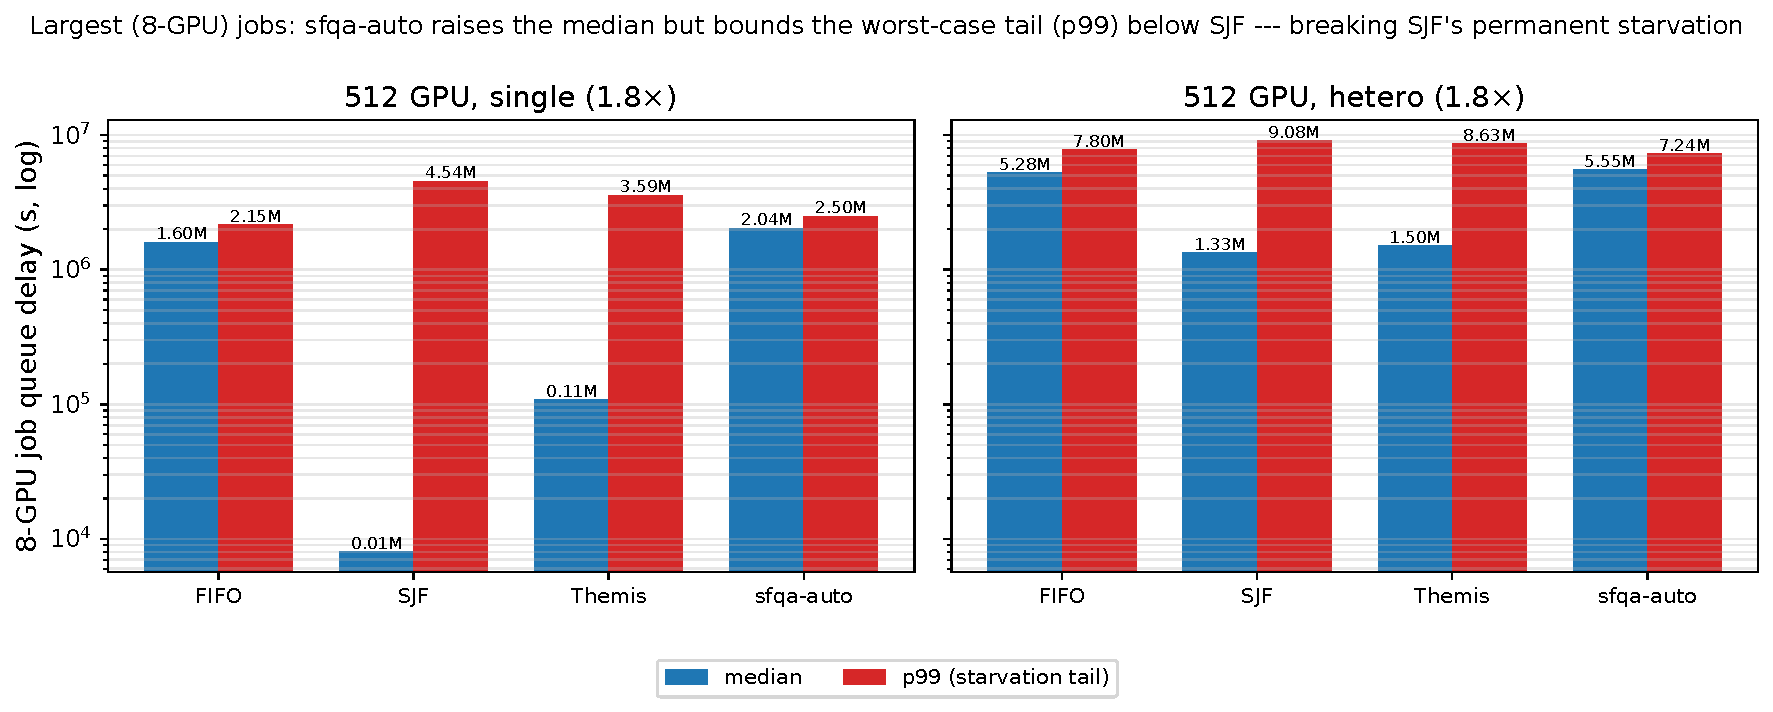
\includegraphics[width=\columnwidth]{Pic/Fig_26.pdf}}
\caption{최대(8-GPU) 작업의 큐 지연 --- 중앙값(파랑) 대 최악 꼬리 p99(빨강), 512 GPU 단일·이종.}
\label{fig:bigjob}
\end{figure}

\paragraph{부차 지표: slowdown(BSLD)}
주축 지표(순서 공정성·wall time·큐 지연) 외에 slowdown 계열의 부차 지표 BSLD(bounded slowdown)도 보고한다. BSLD로 보면 짧은 작업 우선 정책(SJF·Lucid)이 구조적으로 유리하고 SAFA는 열위로 나타난다. 그러나 이는 BSLD가 도착 시점을 무시하고 서비스 시간으로만 지연을 정규화하여 짧은 작업에 본질적으로 유리하기 때문이다 --- 본 연구가 목표로 삼는 공정성은 \eqref{eq:order-fair}의 \textit{도착 순서 공정성}(p1)이지 slowdown 최소화가 아니다. 따라서 BSLD는 주축이 아닌 부차 지표로만 투명하게 보고하며, 정책별 완전한 BSLD 분포는 보충 데이터(\texttt{bsld\_table.csv})로 재현 가능하다.

\begin{figure*}[htb!]
\centerline{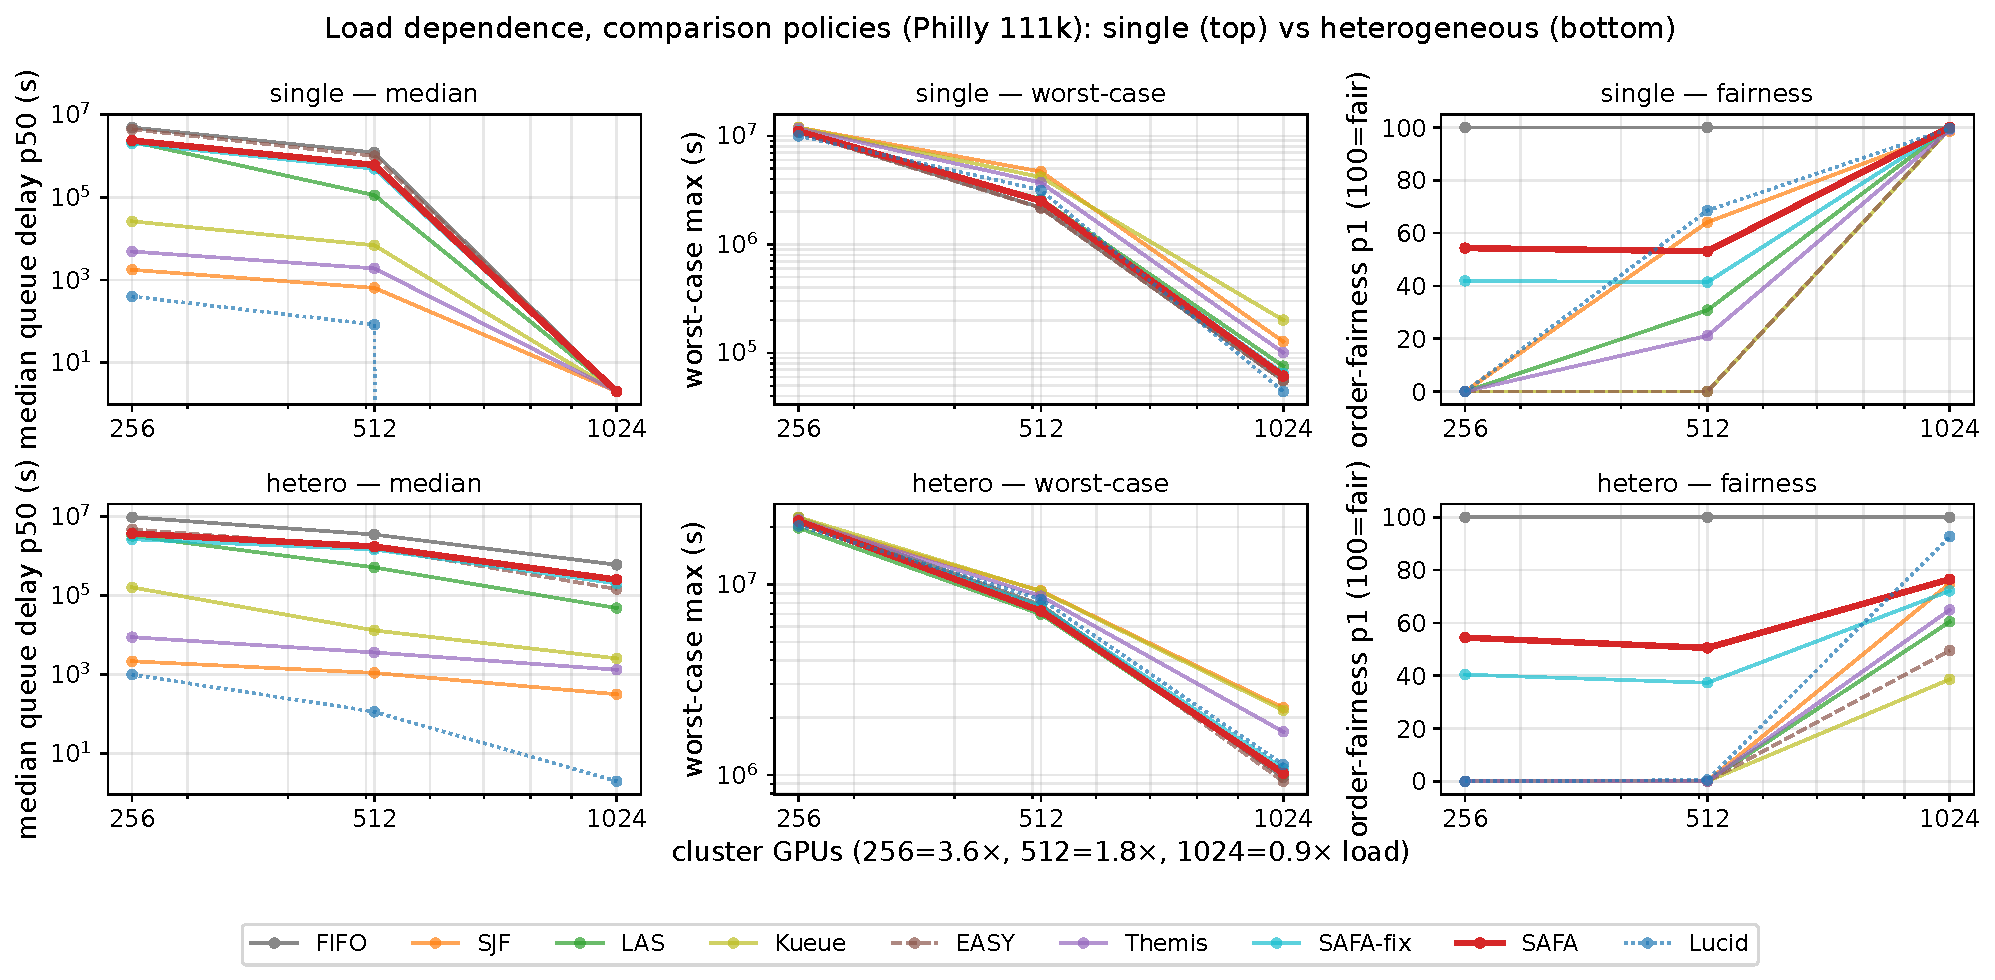
\includegraphics[width=\textwidth]{Pic/Fig_20.pdf}}
\caption{부하 의존성 종합(Philly 111k; 윗줄 단일·아랫줄 이종, 열=q\_p50·q\_max·p1). 본문 \S\ref{eval:main}.}
\label{fig:loadcurve}
\end{figure*}

\paragraph{배치 축과의 직교성: FGD}
배치 베이스라인 FGD에서는 예상과 다른, 그래서 더 유익한 결과가 나왔고 이를 정직하게 보고한다. 표에서 \textbf{FGD와 LAS의 전 지표가 동일}한데, 이는 코드 경로 공유가 아니라 두 겹의 퇴화다 --- (i) 두 정책의 큐 규율이 같고(LAS는 위 항목대로 비차단 FCFS로 퇴화, FGD도 원논문대로 비차단 FCFS), (ii) whole-GPU gang $+$ 지속 과포화에서는 빈 슬롯 자체가 희소해 단편화 인지 배치(ΔF 최소 노드)와 most-allocated가 같은 선택으로 수렴하므로 FGD의 \textit{배치 축이 추가 효과를 내지 못한다}. 따라서 FIFO 대비 54--92\%의 중앙값 단축(512 단일 113K초)은 ``단편화 인지 배치''가 아니라 \textbf{비차단 큐 규율(HOL 스킵)}의 효과로 귀속해야 옳다 --- 그 대가가 과부하에서 하위 1\% 공정성 0 붕괴다(512 이종 p1=0). 이 발견은 두 가지를 시사한다: FGD의 배치 이득은 부분(fractional) GPU 공유·중간 부하라는 원논문 레짐에서 발생하며 본 whole-GPU 과포화 레짐에서는 변별되지 않는다는 것, 그리고 ``빠르지만 굶기는'' 효율 축과 SAFA의 ``빠르면서 공정한'' 균형 축의 대비는 배치가 아니라 큐 규율의 차이라는 것이다. 단편화 인지 배치$+$기아 방지 큐의 결합은 여전히 자연스러운 후속 방향이나, 그 효과 검증에는 부분 공유 레짐이 필요하다. (이종 구성의 노드 타입 혼합은 b200/h100/a100 균등 3분할로 정의했으며, FIFO 기준 다른 베이스라인 측정값과 약 0.8\% 이내로 일치한다.)

\begin{figure*}[htb!]
\centerline{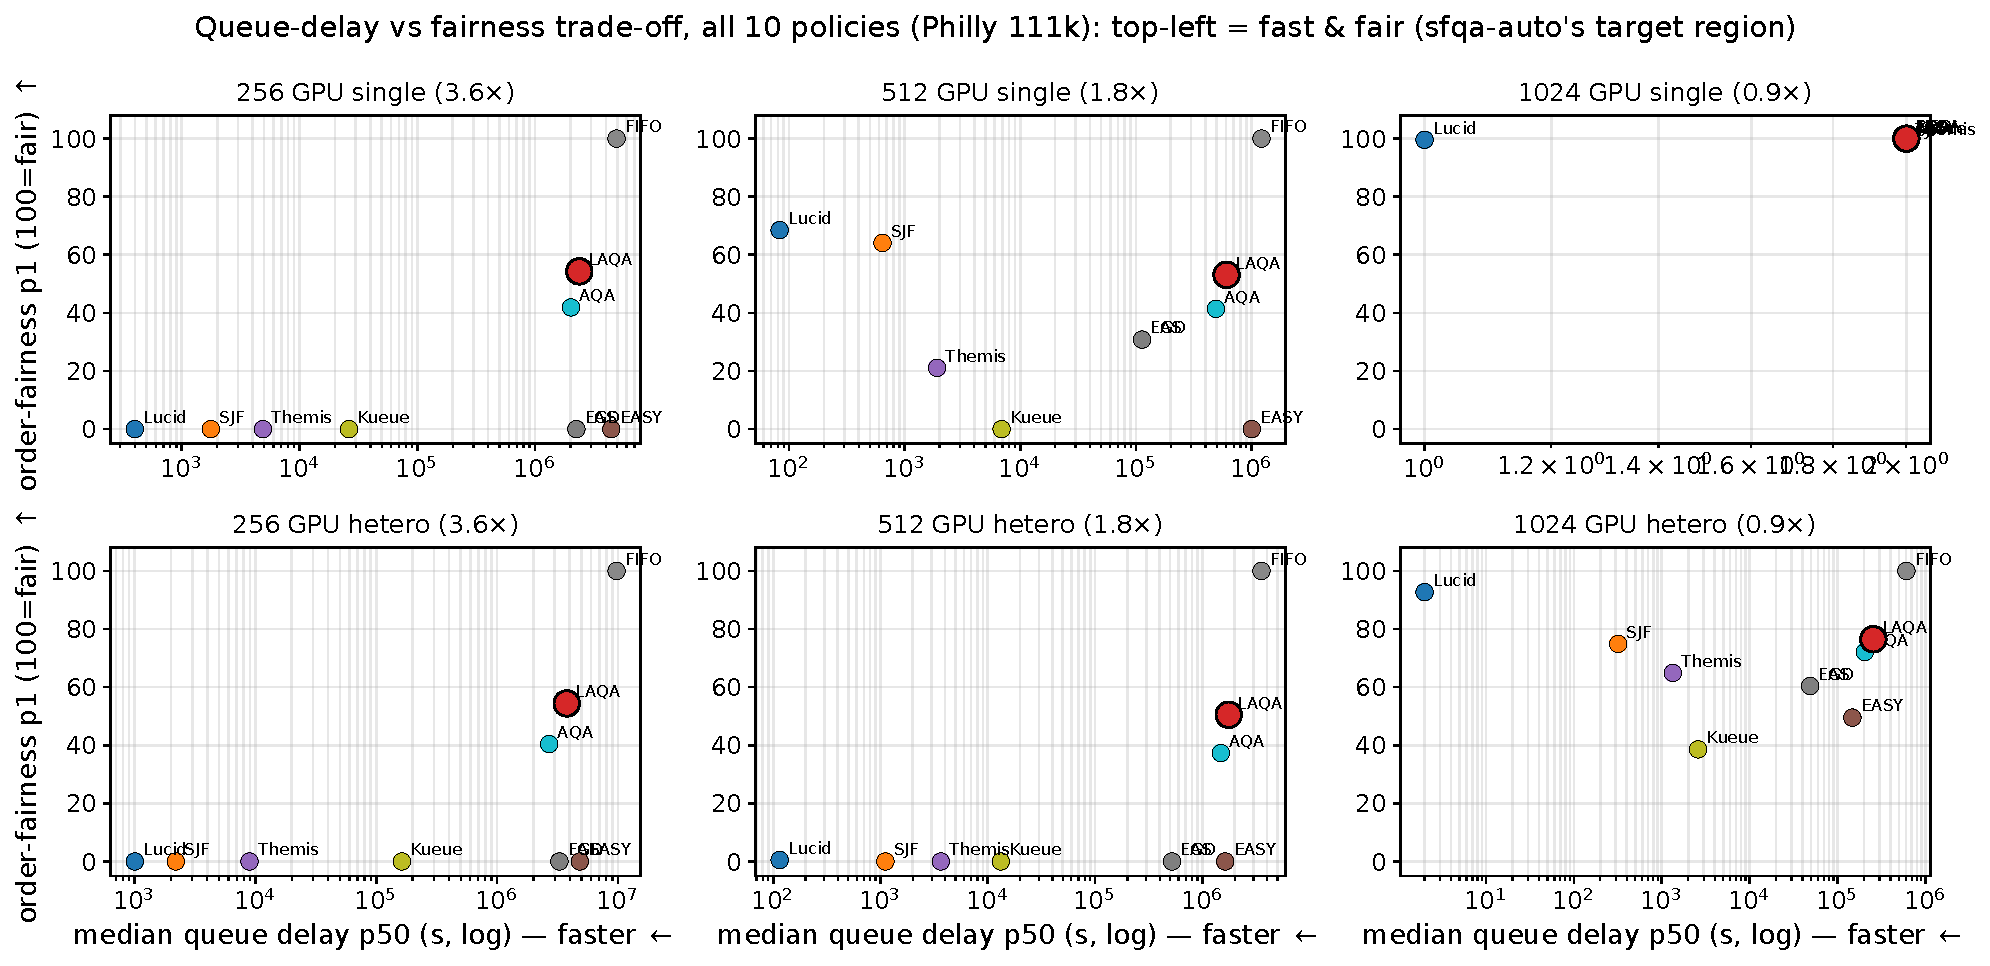
\includegraphics[width=\textwidth]{Pic/Fig_25.pdf}}
\caption{큐 지연 대 공정성 트레이드오프(Philly 111k; 윗줄 단일·아랫줄 이종, 좌상단=빠르고 공정). 마커 구획: 검정 사각=기준선 FIFO, 회색=어드미션 순서 정책 6종, 청색=SAFA 계열, 연회 삼각=배치 축 참고 FGD --- \S\ref{eval:impl}의 층위 분류. 본문 \S\ref{eval:main}.}
\label{fig:tradeoff}
\end{figure*}

\begin{table*}[htb!]
\centering
\caption{단일(동종) 클러스터 결과(Philly 111k; 256/512/1024\,GPU $=$ 3.6/1.8/0.9$\times$ 부하). 지표 정의는 \S\ref{eval:sim}, $q_{\max}$는 그림 \ref{fig:loadcurve}. 행 구획: 기준선(FIFO)/어드미션 순서 정책(동일 층위 비교군)/SAFA 계열/배치 축 참고(FGD) --- \S\ref{eval:impl}의 층위 분류.}
\small
\begin{tabular}{@{}l@{\hspace{1.6em}}rrr@{\hspace{1.6em}}rrr@{\hspace{1.6em}}rrr@{}}
\toprule
 & \multicolumn{3}{c}{\textbf{q\_p50 (s)}} & \multicolumn{3}{c}{\textbf{p1}} & \multicolumn{3}{c}{\textbf{Alloc (\%)}} \\
\cmidrule(lr){2-4}\cmidrule(lr){5-7}\cmidrule(lr){8-10}
\textbf{정책} & 256 & 512 & 1024 & 256 & 512 & 1024 & 256 & 512 & 1024 \\
\midrule
\multicolumn{10}{@{}l}{\textit{무개입 기준선(base) --- SAFA를 끈 상태, 모든 delta의 분모:}} \\
FIFO        & 4.9M & 1.2M & 2   & 100 & 100 & 100 & 99 & 99 & 76 \\
\midrule
\multicolumn{10}{@{}l}{\textit{어드미션 순서 정책(``어떤 것을 먼저'') --- SAFA와 동일 층위의 비교군:}} \\
SJF         & 1.8K & 643  & 2   & 0   & 64  & 99  & 99 & 99 & 76 \\
LAS         & 2.2M & 113K & 2   & 0   & 31  & 100 & 100 & 99 & 75 \\
Kueue       & 26K  & 6.9K & 2   & 0   & 0   & 100 & 99 & 99 & 76 \\
EASY        & 4.4M & 1.0M & 2   & 0   & 0   & 100 & 99 & 99 & 76 \\
Themis      & 4.9K & 1.9K & 2   & 0   & 21  & 99  & 99 & 99 & 76 \\
Lucid       & 399  & 83   & 0   & 0   & 69  & 100 & 100 & 99 & 63 \\
\midrule
SAFA(고정 α)  & 2.0M & 492K & 2   & 42  & 41  & 100 & 99 & 99 & 76 \\
\textbf{SAFA} & 2.4M & 607K & 2 & 54 & 53 & 100 & 99 & 99 & 76 \\
\midrule
\multicolumn{10}{@{}l}{\textit{배치 축 참고 --- 큐는 FCFS, SAFA와 직교(본 레짐에선 LAS와 동일):}} \\
FGD         & 2.2M & 113K & 2   & 0   & 31  & 100 & 100 & 99 & 75 \\
\bottomrule
\end{tabular}
\label{tab:sim-single}
\end{table*}

\begin{table*}[htb!]
\centering
\caption{이종(heterogeneous) 클러스터 결과(열 의미는 표 \ref{tab:sim-single}과 동일).}
\small
\begin{tabular}{@{}l@{\hspace{1.6em}}rrr@{\hspace{1.6em}}rrr@{\hspace{1.6em}}rrr@{}}
\toprule
 & \multicolumn{3}{c}{\textbf{q\_p50 (s)}} & \multicolumn{3}{c}{\textbf{p1}} & \multicolumn{3}{c}{\textbf{Alloc (\%)}} \\
\cmidrule(lr){2-4}\cmidrule(lr){5-7}\cmidrule(lr){8-10}
\textbf{정책} & 256 & 512 & 1024 & 256 & 512 & 1024 & 256 & 512 & 1024 \\
\midrule
\multicolumn{10}{@{}l}{\textit{무개입 기준선(base):}} \\
FIFO        & 9.7M & 3.6M & 607K & 100 & 100 & 100 & 99 & 99 & 97 \\
\midrule
\multicolumn{10}{@{}l}{\textit{어드미션 순서 정책(``어떤 것을 먼저'') --- 동일 층위 비교군:}} \\
SJF         & 2.2K & 1.1K & 319  & 0   & 0   & 75  & 99 & 99 & 96 \\
LAS         & 3.3M & 521K & 49K  & 0   & 0   & 60  & 100 & 99 & 95 \\
Kueue       & 163K & 13K  & 2.6K & 0   & 0   & 39  & 100 & 99 & 95 \\
EASY        & 4.8M & 1.6M & 148K & 0   & 0   & 50  & 99 & 99 & 96 \\
Themis      & 8.9K & 3.7K & 1.3K & 0   & 0   & 65  & 100 & 99 & 96 \\
Lucid       & 1.0K & 115  & 2    & 0   & 1   & 93  & 100 & 99 & 94 \\
\midrule
SAFA(고정 α)  & 2.7M & 1.5M & 205K & 40  & 37  & 72  & 99 & 99 & 96 \\
\textbf{SAFA} & 3.8M & 1.8M & 256K & 54 & 50 & 77 & 99 & 99 & 96 \\
\midrule
\multicolumn{10}{@{}l}{\textit{배치 축 참고(직교 --- 본 레짐에선 LAS와 동일):}} \\
FGD         & 3.3M & 521K & 49K  & 0   & 0   & 60  & 100 & 99 & 95 \\
\bottomrule
\end{tabular}
\label{tab:sim}
\end{table*}

\paragraph{활용도 검증}
SAFA의 중앙값·공정성 이득이 GPU를 놀려서 얻은 것이 아니다(표 \ref{tab:sim-single}·\ref{tab:sim}의 Alloc 열). 동일 엔진의 10개 행(기준선 1·큐 정책 6·SAFA 2·배치 참고 1)은 모두 고정 요청 갱(gang) 작업을 비선점으로 배치하므로, 임계·과부하(256·512 GPU)에서 평균 99\% 안팎의 GPU 할당률을 유지한다 --- 즉 이들 간 차이는 자원을 놀린 결과가 아니라 순수한 큐 순서·배치 효과다(저부하 1024에서는 수요가 얕아 모든 정책이 동반 하락). SAFA는 할당률을 떨어뜨리지 않으면서 효율과 공정성의 균형을 달성한다.

종합하면, 이 경향은 SAFA의 설계와 일관된다. SAFA가 \eqref{eq:auto-alpha}처럼 나이 가중 계수를 큐 나이 통계로 무튜닝 정규화하므로, 부하가 0.9$\times$에서 3.6$\times$로, 또 단일에서 이종으로 바뀌어도 동일한 코드와 설정으로 하위 1\% 공정성을 50.5--76.5 수준으로 유지한다 --- 다른 어떤 빠른 정책도 보이지 못한 안정성이다. 운영 관점에서 SAFA는 (i) 워크로드별 계수 튜닝이 불필요하고, (ii) 단일 승급 $O(n)$ 연산으로 부하와 무관하게 경량이며, (iii) 약 99\%의 GPU 할당률을 유지하면서 효율과 공정성의 균형을 달성한다. 따라서 기존 클러스터 스케줄러를 교체하지 않고 그 위에 부담 없이 통합될 수 있는, 본 평가에서 유일한 실용적 후보다.

\subsection{무튜닝의 순효과: 고정 $\alpha$ 대비 ablation}\label{eval:ablation}
무튜닝이 가져온 순효과를 \textit{같은 큐 전처리 골격} 안에서 격리하기 위해, 고정 계수 SAFA(고정 $\alpha$)와 무튜닝 SAFA를 6구성 전체에서 직접 대비한다(표 \ref{tab:ablation}). 두 변형은 식 \eqref{eq:01}/\eqref{eq:auto-pstar}의 동일한 $P^*$ 구조와 단일 승급 절차를 공유하며, 유일한 차이는 나이 가중 계수를 \textit{사전에 고정한 단일 값}으로 두느냐, \textit{큐 통계에서 매 패스 유도}하느냐다. 여기서 SAFA(고정 $\alpha$)는 \textbf{워크로드별 최적 $\alpha$가 아니라 모든 구성에 공통으로 쓴 단일 고정 설정 $\alpha=0.13889$(\S\ref{algo:intro} 예시값의 10배 --- C++ 구현 기본값)}임을 분명히 밝힌다 --- 즉 이 표는 ``재튜닝 없이 단일 무튜닝 규칙이 단일 고정값보다 공정성을 일관되게 지키는가''라는 1차 질문에 답한다. 이어 \S\ref{eval:ablation:grid}에서 구성별로 $\alpha$를 그리드 탐색한 \textit{워크로드별 최적} 고정값과 대비하여, 그 비교의 정직한 전모 --- 0.01--2.0 그리드 안에선 무튜닝이 모두를 능가하나, 그리드를 미세 영역까지 넓히면 고정 $\alpha$도 frontier의 다른 점에 도달하며, 무튜닝의 가치는 지배가 아니라 \textit{탐색 없는 일관 균형점}임 --- 를 제시한다.

표 \ref{tab:ablation}이 보이듯, 무튜닝 SAFA는 6구성 모두에서 하위 1\% 순서 공정성(p1)을 고정 $\alpha$ 대비 동등 이상으로 유지한다 --- 경합이 깊은 256·512 구성에서 p1을 단일에서 41.9$\to$54.3, 41.4$\to$53.1로, 이종에서 40.4$\to$54.4, 37.3$\to$50.5로 끌어올렸고, 큐가 얕은 1024 구성에서도 동등(단일 100$=$100)하거나 향상(이종 72.1$\to$76.5)했다. 이 공정성 향상의 대가는 작은 중앙값 양보(예: 512 이종 q\_p50 1.48M$\to$1.76M초)이며, 평균 GPU 할당률은 두 변형이 사실상 동일하다(전 구성 0.1\%p 이내). 요컨대 \textit{단일 고정 $\alpha$를 워크로드마다 다시 고를 필요 없이}, 큐에서 유도한 무튜닝 계수만으로 부하·이질성 전반에서 공정성이 더 안정적으로 유지된다.

\begin{table}[htb!]
\centering
\caption{고정 $\alpha$ 대비 무튜닝 SAFA ablation(6구성). 지표 정의는 \S\ref{eval:sim}.}
\label{tab:ablation}
\small
\begin{tabular}{@{}ll@{\hspace{1.0em}}rr@{\hspace{1.0em}}rr@{\hspace{1.0em}}rr@{}}
\toprule
 & & \multicolumn{2}{c}{\textbf{q\_p50 (s)}} & \multicolumn{2}{c}{\textbf{p1}} & \multicolumn{2}{c}{\textbf{Alloc}} \\
\cmidrule(lr){3-4}\cmidrule(lr){5-6}\cmidrule(lr){7-8}
\textbf{구성} & \textbf{GPU} & 고정\,$\alpha$ & SAFA & 고정\,$\alpha$ & SAFA & 고정\,$\alpha$ & SAFA \\
\midrule
\multirow{3}{*}{단일} & 256  & 2.0M & 2.4M & 41.9 & \textbf{54.3} & 99.1 & 99.0 \\
                     & 512  & 492K & 607K & 41.4 & \textbf{53.1} & 98.8 & 98.8 \\
                     & 1024 & 2    & 2    & 100  & 100           & 75.6 & 75.7 \\
\midrule
\multirow{3}{*}{이종} & 256  & 2.7M & 3.8M & 40.4 & \textbf{54.4} & 99.1 & 99.1 \\
                     & 512  & 1.5M & 1.8M & 37.3 & \textbf{50.5} & 99.0 & 99.0 \\
                     & 1024 & 205K & 256K & 72.1 & \textbf{76.5} & 95.8 & 95.8 \\
\bottomrule
\end{tabular}
\end{table}

\subsubsection{워크로드별 최적 고정 $\alpha$와의 대비(강화판)}\label{eval:ablation:grid}
앞 비교의 고정 $\alpha$는 모든 구성에 공통인 단일값이었다. 더 강한 질문은 ``\textit{구성마다} $\alpha$를 최적으로 골라 줘도 무튜닝이 따라잡히는가''이다. 이를 답하기 위해 6구성 각각에서 SAFA(고정 $\alpha$)를 16점 그리드($\alpha$를 0.01에서 2.0까지 부등간격으로\footnote{$\alpha \in \{0.01, 0.02, 0.05, 0.1, 0.139, 0.2, 0.3, 0.5, 0.7, 0.9, 1.0, 1.2, 1.4, 1.6, 1.8, 2.0\}$.})로 스윕하여, 그 구성에서 \textit{도달 가능한 최선의 하위 1\% 순서 공정성}(p1)을 내는 고정 $\alpha$를 구하고 무튜닝 SAFA와 대비했다(표 \ref{tab:ablation-grid}, 그림 \ref{fig:ablation-grid}). 0.01--2.0 그리드 안에서는 부하가 존재하는 5개 구성 전부에서 어떤 고정 $\alpha$도 무튜닝 SAFA의 p1에 못 미치며(최선 고정값 대비 $+4.4$--$12.8$점, 예: 512 이종 39.1 대 50.5), 고정 $\alpha$의 p1이 두 자릿수 $\alpha$ 범위에서 좁은 띠(예: 36.4--39.1)에 갇힌다. 그러나 \textbf{이 그리드의 하한이 결론을 만들지 않는지 스스로 검증했다} --- 무튜닝 $\alpha_{\text{eff}}=1/(A_{\text{ref}}R_{\min})$는 과포화에서 $10^{-3}$ 이하로 내려가므로, 그리드를 $10^{-4}$까지 확장해 재실행하면 \textit{고정 $\alpha$도 결국 FIFO 쪽으로 올라간다}: 512 단일에서 $\alpha{=}10^{-4}$는 p1 87.5($q_{p50}$ 1.11M초), $3{\times}10^{-4}$는 61.0(626K초)이다. 즉 \textbf{고정 $\alpha$ 역시 --- 전체 정렬 aging의 $w$와 마찬가지로(\S\ref{eval:ablation:comp}) --- FIFO(공정·느림)와 그리디(빠름·추월)를 잇는 보간 노브}이고, ``도달 불가능한 동작점''은 없다. 무튜닝의 가치는 frontier 독점이 아니라 다음 두 가지다. 첫째, \textbf{노브의 위험한 민감성 제거}: 고정 $\alpha$의 p1은 $10^{-4}$에서 $3{\times}10^{-3}$ 사이 한 자릿수 반 만에 87$\to$46(단일)으로 급변하는 절벽이며, 그 절벽의 위치가 워크로드의 \textit{절대 나이 스케일}에 결합돼 있어 트레이스가 바뀌면 같은 $\alpha$가 전혀 다른 동작점을 준다(\S\ref{sec:coeff}의 분포별 7배 변동과 같은 뿌리). 무튜닝은 이 결합을 $A_{\text{ref}}$ 정규화로 끊고 노브 없이 균형점(512 단일 53.1/607K, 이종 50.5/1.76M --- 인접 고정점들과 상호 비지배)에 도달한다. 미세 고정값의 교차-트레이스 거동도 직접 쟀다: $\alpha{=}3{\times}10^{-4}$는 세 트레이스에서 p1 61--67로 살아남아 \textit{frontier의 효율 쪽 한 점}에 일관 안착한다 --- 즉 잘 고른 고정값도 무너지지는 않는다. 무튜닝의 차별은 그보다 공정 쪽 균형점(p1 50.5/83.9/98.4)을 \textbf{노브 없이} 잡고, 고정 $\alpha$ 대비 p1을 세 트레이스 전부에서 13--25점 상회한다는 데 있다. 둘째, \textbf{재튜닝 불요의 일관성}: 같은 코드·설정으로 6구성·세 트레이스 전부에서 이 균형점이 유지된다. 이 우위의 대가는 작은 중앙값 양보(그리드-내 최선 고정값 대비 q\_p50 $+18$--$32$\%)로, 우리는 이를 숨기지 않는다.

이 p1 우위가 통계적으로 유의함도 확인했다. 시뮬레이터가 결정적 전체 트레이스 재생이라 시드 무작위성이 없으므로, 변동성은 잡 모집단에 대한 부트스트랩(1,000회 복원추출; 순서 공정성 점수는 전체 모집단에서 1회 계산해 잡 속성으로 고정)으로 추정했다. 512 구성에서 무튜닝 SAFA의 p1 95\% 신뢰구간([52.5,\,53.3] 단일 / [50.4,\,50.7] 이종)은 \textit{공통 고정} $\alpha{=}0.13889$의 구간([40.6,\,42.0] / [37.2,\,37.5])과 \textbf{겹치지 않는다}(부트스트랩은 이 두 구성으로 수행 --- 그리드-내 최선 고정값 42.4/39.1과의 점추정 격차 10.7--11.4점도 CI 폭 $\pm$0.7의 10배 이상이라 같은 결론이나, 그 구성의 CI는 별도 산출하지 않았음을 명시한다). 미세 $\alpha$ 영역과의 관계는 위 frontier 논의 참조. 이 부트스트랩이 재는 것은 잡 모집단에 대한 분위 추정의 변동이며, 도착 섭동·트레이스 윈도우 선택 같은 \textit{정책 거동 수준}의 변동성은 포착하지 않는다(결정적 재생의 한계로 명시해 둔다).

\subsubsection{성분 ablation: $R$ 결합을 끄면 무엇이 남는가}\label{eval:ablation:comp}
\S\ref{sec:coeff}는 SAFA가 고전 priority aging과 갈리는 첫 번째 지점으로 \textit{불가분 갱 자원에 대한 $R$ 결합}을 들었다. 이 주장을 성분 수준에서 격리하기 위해, 같은 단일 승급 골격에서 두 변형을 추가로 평가했다(표 \ref{tab:ablation-comp}): (i) \textbf{$R\equiv1$} --- 무튜닝 SAFA에서 자원 적합도 결합만 제거(상대 나이 정규화는 유지), (ii) \textbf{고전 aging} --- 절대 나이$\times$고정 $\alpha$($=0.13889$), $R$ 없음, 항상 발동. 결과는 부분적 열화가 아니라 \textbf{완전한 퇴화}다: 두 변형 모두 세 구성 전부에서 중앙값 대기가 FIFO와 \textit{동일한 값까지} 일치하고(예: 512 이종 3.55M초 $=$ FIFO) p1$\approx$100, 즉 \textbf{FIFO와 거동이 동치}가 된다. 메커니즘은 구조적이다 --- 도착순 큐에서는 base 우선순위 $P$(큐 위치 단조 감소)와 나이(선두가 항상 최대) \textit{둘 다} 큐 선두에서 최대이므로, $R$이 없으면 $P^*$의 argmax가 항상 선두가 되어 단일 승급이 \textit{한 번도 발화하지 않는다}. $R$만이 ``지금 비는 자리에 맞는 뒤쪽 작업''에 선두를 넘어설 이유를 제공한다. 따라서 단일 승급 구조 안에서 SAFA의 비-FIFO 거동 전부는 $R$ 결합에서 나오며, \textit{$R$ 없는 aging은 본 구조에서 항등}이다.

이 동치는 단일 승급$+$위치 단조 $P$ 구조에 대한 결과이므로, \textit{전체 재정렬형} 고전 aging --- Slurm multifactor처럼 큐 전체를 점수로 정렬하는 형태 --- 는 별도로 측정했다. 절대 나이 단독의 전체 정렬은 정의상 도착순과 같아 FIFO와 동치임을 측정으로 확인했고($q_{p50}$까지 동일), 나이$+$크기 가중 $s_j = w\,\hat A_j + (1{-}w)(1{-}\text{gpu}_j/8)$의 전체 정렬(Slurm의 age$+$size factor에 대응, 무정보 조건 유지)은 $w$에 따라 FIFO(공정·느림)와 크기-선별 그리디(빠름·불공정)를 잇는 \textit{보간 곡선}을 그린다: 512 이종에서 $w{=}0.5$는 p1 $0$($q_{p50}$ 391K초), $w{=}0.65$는 p1 $54.3$(2.01M초), $w{=}0.75$는 p1 $72.5$(2.76M초)다. 정직하게 말해, \textbf{$w$를 워크로드별로 맞추면 전체 정렬 aging도 SAFA와 유사한 효율--공정성 frontier에 도달한다} --- SAFA(p1 50.5, 1.76M초)는 이 곡선의 $w{=}0.6$--$0.65$ 인접점들과 비교해 지배당하지 않는 균형점이지만, frontier를 독점하지도 않는다. 차별점은 frontier가 아니라 \textbf{그 균형점에 도달하는 방식}이다: (i) $w$는 0.5에서 0.65 사이에서 p1이 0$\to$54로 급변하는 \textit{절벽형 노브}다. 같은 Philly 안의 세 구성에서는 $w{=}0.65$가 안정적이지만(p1 54--57), \textbf{트레이스를 바꾸면 이전이 실제로 실패한다} --- 같은 $w{=}0.65$(와 0.5·0.75 전부)가 Helios에서 p1 0·\texttt{lt50} 19.9\%, Alibaba에서 p1 0·12.5\%로 완전히 붕괴하는 반면, 무튜닝 SAFA는 동일 코드로 두 트레이스에서 p1 83.9·98.4를 유지한다. 절벽의 위치가 갱 크기 분포·나이 스케일에 결합돼 있다는 우려가 실측으로 확정된 것이다 --- \S\ref{sec:coeff}가 고정 $\alpha$에서 보인 것과 같은 종류의 민감성이다. SAFA는 노브 없이 같은 영역의 균형점에 자동 도달하며, \textit{같은 p1대에서 중앙값이 9--17\% 빠르다}(512 단일 607K 대 732K, 이종 1.76M 대 2.01M, 256 이종 3.77M 대 4.13M초). (ii) 크기 factor $(1{-}\text{gpu}_j/8)$는 \textit{정적} 신호인 반면 SAFA의 $R_j$는 \textit{지금 비는 자리}를 보는 상태-인지 신호다 --- 같은 큰 작업도 자리가 나면 승급 대상이 된다. 요컨대 ``aging은 고전''이라는 반론에 대한 답은 두 겹이다: 단일 승급 구조에서는 $R$ 결합 없이 aging이 발화하지 않고(위 동치), 전체 정렬 구조에서는 발화하되 워크로드-민감 가중 노브를 요구한다 --- 본 기여는 그 노브 없이 균형점에 도달하는 무튜닝 메커니즘이다. 같은 검증을 aging 밖의 가장 단순한 무정보 대안에도 적용했다: 작업당 추월 상한 $K$를 둔 비차단 FCFS(bounded-skip)는 $K$에 따라 FIFO($K{=}8$: p1 99.4, 3.58M초)와 그리디($K{=}512$: p1 0, 839K초)를 잇는 또 하나의 보간 노브이며, 측정된 어느 $K$도 SAFA(50.5, 1.76M초)를 지배하지 못한다($K{=}64$는 p1 82.2를 주지만 중앙값이 3.46M초로 SAFA의 두 배다). 나이를 아예 빼고 ``fit하는 가장 오래된 작업 1건만 승급''하는 무예약 백필 대조(fit-oldest)도 측정했다: 중앙값은 445K초로 빠르지만 p1 0·\texttt{lt50} 7.6\%로 공정성이 무너진다 --- fit 신호 단독이 아니라 \textit{나이-정규화된 fit}이 공정 균형점을 만든다는 성분 분리다.

\begin{table}[htb!]
\centering
\caption{성분 ablation --- 단일 승급 구조에서 $R$ 결합 제거 시 FIFO 퇴화, 전체 정렬 aging은 가중 $w$ 보간 곡선(Philly 전체, 3구성). 본문 \S\ref{eval:ablation:comp}.}
\label{tab:ablation-comp}
\footnotesize
\begin{tabular}{@{}ll@{\hspace{1.0em}}rr@{\hspace{1.0em}}rr@{}}
\toprule
 & & \multicolumn{2}{c}{\textbf{q\_p50 (s)}} & \multicolumn{2}{c}{\textbf{p1}} \\
\cmidrule(lr){3-4}\cmidrule(lr){5-6}
\textbf{구성} & \textbf{변형} & 변형 & SAFA & 변형 & SAFA \\
\midrule
\multirow{3}{*}{단일 512} & $R\equiv1$ & 1.22M ($=$FIFO) & 607K & $\approx$100 & 53.1 \\
                          & 고전 aging(단일승급) & 1.22M ($=$FIFO) & 607K & $\approx$100 & 53.1 \\
                          & 전체정렬 aging($w{=}0.75$) & 1.05M & 607K & 74.3 & 53.1 \\
\midrule
\multirow{3}{*}{이종 512} & $R\equiv1$ & 3.55M ($=$FIFO) & 1.76M & $\approx$100 & 50.5 \\
                          & 고전 aging(단일승급) & 3.55M ($=$FIFO) & 1.76M & $\approx$100 & 50.5 \\
                          & 전체정렬 aging($w{=}0.75$) & 2.76M & 1.76M & 72.5 & 50.5 \\
\midrule
\multirow{3}{*}{이종 256} & $R\equiv1$ & 9.75M ($=$FIFO) & 3.77M & $\approx$100 & 54.4 \\
                          & 고전 aging(단일승급) & 9.75M ($=$FIFO) & 3.77M & $\approx$100 & 54.4 \\
                          & 전체정렬 aging($w{=}0.75$) & 6.95M & 3.77M & 72.2 & 54.4 \\
\bottomrule
\end{tabular}
\end{table}

\begin{table}[htb!]
\centering
\caption{구성별 0.01--2.0 그리드 내 최선 고정 $\alpha$ 대 무튜닝 SAFA(그림 \ref{fig:ablation-grid}). $\alpha<0.01$ 미세 영역은 FIFO 쪽 보간으로 올라간다(본문 \S\ref{eval:ablation:grid}, 예: 512 단일 $\alpha{=}10^{-4}$에서 p1 87.5).}
\label{tab:ablation-grid}
\small
\begin{tabular}{@{}ll@{\hspace{0.8em}}rr@{\hspace{0.8em}}rr@{}}
\toprule
 & & \multicolumn{2}{c}{\textbf{최적 고정 $\alpha$}} & \multicolumn{2}{c}{\textbf{SAFA (무튜닝)}} \\
\cmidrule(lr){3-4}\cmidrule(lr){5-6}
\textbf{구성} & \textbf{GPU} & p1\,($\alpha^\ast$) & q\_p50 & p1 & q\_p50 \\
\midrule
\multirow{3}{*}{단일} & 256  & 42.9\,(0.02) & 2.0M & \textbf{54.3} & 2.4M \\
                     & 512  & 42.4\,(0.01) & 490K & \textbf{53.1} & 607K \\
                     & 1024 & 100\,(any)   & 2    & 100           & 2    \\
\midrule
\multirow{3}{*}{이종} & 256  & 41.6\,(0.5)  & 2.9M & \textbf{54.4} & 3.8M \\
                     & 512  & 39.1\,(0.01) & 1.4M & \textbf{50.5} & 1.8M \\
                     & 1024 & 72.1\,(0.7)  & 201K & \textbf{76.5} & 256K \\
\bottomrule
\end{tabular}
\end{table}

\begin{figure*}[htb!]
\centerline{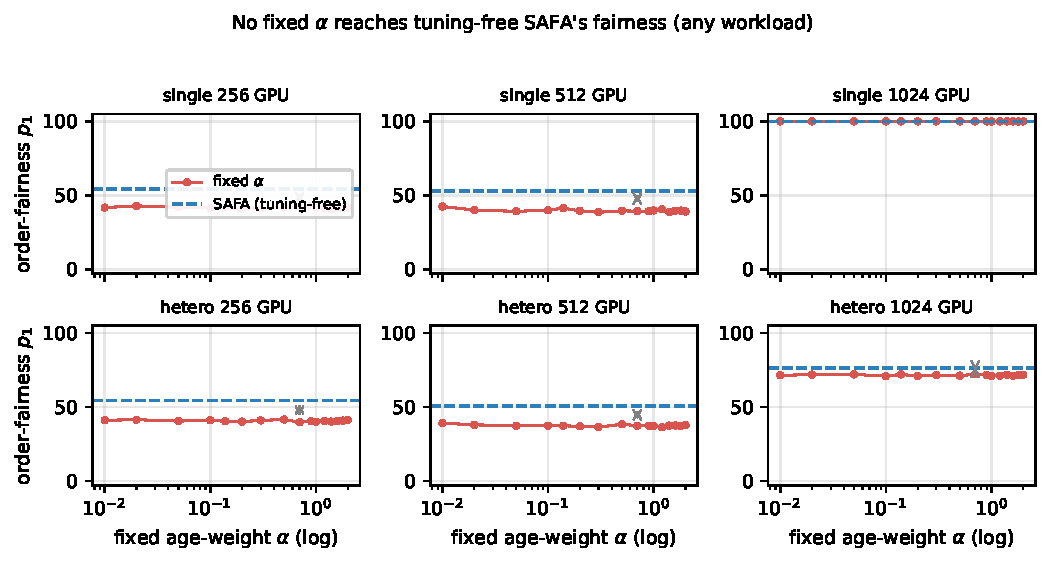
\includegraphics[width=\textwidth]{Pic/fig_ablation_grid.pdf}}
\caption{고정 $\alpha$ 스윕 하위 1\% 순서 공정성(빨강) 대 무튜닝 SAFA(파란 점선), 6구성. 본문 \S\ref{eval:ablation:grid}.}
\label{fig:ablation-grid}
\end{figure*}

\subsection{강건성과 일반화}\label{eval:robust}
주 결과(\S\ref{eval:main})와 ablation(\S\ref{eval:ablation})이 보인 핵심 대비 --- \textit{이종·과부하에서 정보-우위 베이스라인이 아사(공정성 붕괴)를 겪는 반면 SAFA는 큐 정보만으로 이를 예방한다} --- 가 평가 설계의 산물이 아니라 현상의 산물임을 네 축에서 시험한다: (i) 합성 모델 계수에 대한 민감도, (ii) 독립 트레이스로의 일반화, (iii) 시뮬레이터 구현의 충실도, (iv) 코어 배치 스케줄러에 대한 무관성(어드미션-계층 정체성의 직접 검증). 통계적 유의성은 이미 \S\ref{eval:ablation:grid}의 잡-레벨 부트스트랩 신뢰구간(무튜닝과 고정 $\alpha$의 p1 구간 비중첩)이 뒷받침한다.

\subsubsection{합성 계수 민감도 ($\pm 50\%$)}\label{eval:robust:sens}
동일 엔진 베이스라인 중 SJF·EASY·Themis는 완벽한 duration 예측(oracle)을, Lucid는 정확한 잡별 utilization 프로파일을 \textit{비용·오차 없이} 제공받는다 --- 이는 이들 정보-우위 정책에 \textit{유리한} 방향의 이상화이므로, 무정보 SAFA가 이들과 경쟁한다는 결론은 \textit{보수적}이다(편향이 SAFA에 불리). 이 결론이 합성 계수의 특정 선택에 의존하지 않음을 보이기 위해, 합성 파라미터를 각각 $\pm50\%$ 흔들어 512 단일·이종에서 \textbf{전 정책}을 재평가했다(표 \ref{tab:sens}, 그림 \ref{fig:sens-robust}). 타입 속도계수와 수명주기 오버헤드는 \textit{모든} 정책의 거동에 영향을 주므로 표의 10행(베이스라인 8개와 SAFA 두 변형) 전부를 교란 하에서 재실행했고, Lucid의 collocation 슬로다운(SS)은 \textit{Lucid에만} 작용하므로 Lucid에 한해 추가로 $\pm50\%$ 교란했다. 핵심 부호는 교란 전 구간에서 불변이다: 무튜닝 SAFA의 하위 1\% 공정성이 고정 $\alpha$를 능가한다는 관계가 유지되며(무튜닝 p1 $49.7$--$53.1$ 대 고정 $36.9$--$41.4$ --- 표는 이종, 단일 수치는 보충자료), 특히 속도계수 $\pm50\%$가 이종 무튜닝 p1을 1점 미만으로만 움직여 결론이 합성 속도 모델의 인공물이 아님을 확인했다. 이종 과부하에서 정보-우위 베이스라인의 공정성 붕괴($p1\!\approx\!0$)도 대체로 유지되나, 한 가지 예외를 정직하게 짚는다 --- Lucid는 속도계수 $-50\%$ 교란에서 p1이 0.7$\to$13.8로 출렁여, 합성 속도계수가 정보-우위 정책의 공정성 \textit{판정 자체}를 흔들 수 있음을 보인다(그래도 SAFA의 49.7과는 자릿수 차이). Lucid 전용 SS $\pm50\%$ 교란에서는 p1 변화가 1점 미만이었다. SAFA의 잔여 내부 상수도 주 엔진 p1 기준으로 직접 흔들었다: base 1.5/3/4는 p1 50--51.5(둔감), $R$ 감쇠 0.05/0.2는 p1 98.3/67.3으로 효율--공정 균형점을 이동시킨다 --- 감쇠는 숨은 워크로드 노브가 아니라(세 트레이스에서 0.1 고정으로 일관) 균형 선호 상수임을 \S\ref{SAFA}에 명시했다. 요컨대 주 대비는 계수 섭동에 견고하되, Lucid 행의 절대값은 합성 계수 의존임을 함께 명시한다.
\begin{table}[htb!]
\centering
\caption{합성 계수 $\pm50\%$ 교란 하의 하위 1\% 순서 공정성 $p1$(512 이종; 그림 \ref{fig:sens-robust}). base 열의 37.4는 본 절 재실행값으로 표 \ref{tab:ablation}의 37.3과 0.1 차이(37.35의 반올림 갈림).}
\label{tab:sens}
\footnotesize
\begin{tabular}{@{}l@{\hspace{0.7em}}rrrrr@{}}
\toprule
\textbf{정책} & base & spd$-$ & spd$+$ & ovh$-$ & ovh$+$ \\
\midrule
FIFO          & 100  & 100  & 100  & 100  & 100  \\
SJF           & 0    & 1.7  & 0    & 0    & 0    \\
LAS           & 0    & 0    & 0    & 0    & 0    \\
Kueue         & 0    & 0    & 0    & 0    & 0    \\
EASY          & 0    & 0    & 0    & 0    & 0    \\
Themis        & 0    & 0    & 0    & 0    & 0    \\
FGD           & 0    & 0    & 0    & 0    & 0    \\
Lucid         & 0.7  & 13.8 & 0.0  & 0.6  & 0.7  \\
SAFA(고정 $\alpha$) & 37.4 & 37.8 & 38.4 & 36.9 & 37.3 \\
\textbf{SAFA} & \textbf{50.5} & \textbf{49.7} & \textbf{50.2} & \textbf{50.8} & \textbf{50.9} \\
\bottomrule
\end{tabular}
\end{table}

\begin{figure}[htb!]
\centerline{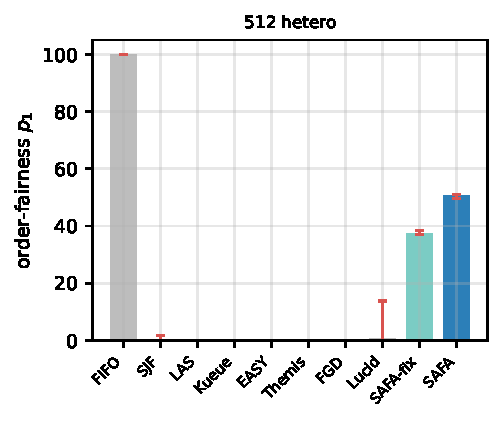
\includegraphics[width=\columnwidth]{Pic/fig_sensitivity.pdf}}
\caption{합성 계수 $\pm50\%$ 교란 하 $p1$(512 이종; 막대=baseline, 수염=교란 min/max). 본문 \S\ref{eval:robust:sens}.}
\label{fig:sens-robust}
\end{figure}

\subsubsection{독립 트레이스로의 일반화}\label{eval:robust:trace}
주 평가는 단일 트레이스(Philly, MS Azure 2017)에 기반하므로, 핵심 경향이 다른 워크로드에서도 재현되는지 독립 트레이스로 시험한다. 먼저 Philly와 출처·시기·하드웨어가 모두 분리된 \textit{사내 쿠버네티스 GPU 클러스터 실측 트레이스}(2024년, A100/A30, 368작업)를 세 부하점(과부하 2.45$\times$/중부하 1.22$\times$/저부하 0.61$\times$)에서 재생했다(표 \ref{tab:inhouse}). 핵심 경향이 재현된다 --- 과부하·임계 부하(8·16 GPU)에서 비차단 비교 정책들(SJF·LAS·Kueue·EASY·Themis·FGD·Lucid)이 모두 하위 1\% 공정성 $p1=0$으로 붕괴하는 반면, 무튜닝 SAFA는 큐 정보만으로 그 아사를 예방해 $p1$ 90--98을 유지한다(고정 $\alpha$보다도 높음). 저부하(32 GPU)로 가면 큐가 얕아져 대부분 정책이 회복하지만, 이종에서는 Themis($p1{=}5.6$)·Lucid($p1{=}0$)가 여전히 무너지는 가운데 SAFA는 93.4를 유지한다 --- 모두 Philly에서 관찰된 ``과부하 붕괴 $\to$ 저부하 회복'' 패턴과 일치한다. 다만 368작업은 Philly(111k)보다 통계력이 약하고($p1=0/100$ 같은 극단 하위 1\% 값이 소표본에서 단일 작업에 좌우될 수 있으며, 소규모·극과부하에서 단일·이종 구분이 큐잉 압력에 묻힘), 이 한계를 메우기 위해 \textbf{대규모 공개 독립 트레이스}로 동일 검증을 추가 수행한다.
이를 위해 \textbf{Helios}\cite{hu2021helios}(SenseTime, SC'21)의 Venus 트레이스 --- Philly와 독립인 또 하나의 대규모 공개 트레이스(GPU 작업 125,303개) --- 에서 동일 스윕을 수행했다(표 \ref{tab:helios}·그림 \ref{fig:helios}, 과부하 이종 80 GPU; 런타임 제약으로 seed-42 50\% 서브샘플; Lucid 포함 10정책). 방법상의 정정을 먼저 정직하게 공개한다: Venus에는 클러스터 용량(80 GPU)을 초과하는 요청(최대 200 GPU, 1.06\%)이 있어, 초기 실행에서 blocking 정책(FIFO·SAFA 계열)은 이 작업에서 영구 차단되어 앞쪽 일부만 완료된 채 측정되는 \textit{모집단 불일치}가 있었다. 본 표는 50\% 서브샘플(62,735작업)에서 용량 초과 666건을 제거한 \textbf{동일 모집단}(62,069작업)으로 10정책 전부를 재실행한 결과다. 결과는 Philly의 구도를 그대로 재현한다 --- \textbf{비차단 정보-우위 정책 전부의 worst-1\% $p1$이 0으로 붕괴}하고 추월 비율 \texttt{lt50\%}도 8.9--21.9\%에 이르는 반면, \textbf{무튜닝 SAFA는 $p1{=}83.9$·\texttt{lt50\%}$\,{=}0.0$}으로 순서 공정성을 유지하며 평균 공정성(98.9)도 비-FIFO 중 최고다(고정 $\alpha$는 63.7/0.05로 그다음 --- 무튜닝 우위도 재현). 효율 축에서는 trade-off가 Philly보다 가파르다: SAFA의 중앙 대기는 FIFO 대비 15\% 짧지만(37.9M 대 44.6M초) 비차단 그리디(수십 초$\sim$1.1M초)와는 자릿수가 다르다 --- 대형 gang(평균 6.7 GPU)이 큐를 지배하는 이 트레이스에서 순서 보존의 효율 비용은 크고, 우리는 이를 숨기지 않는다(절대값은 80 GPU 스트레스 설정의 산물). 기아 꼬리(q\_max)로는 blocking 계열 78--91M초와 비차단 64--85M초가 겹치는 범위여서, 비차단의 낮은 중앙값이 최악 꼬리를 더 키우지는 않는 대신 그 비용을 추월(\texttt{lt50\%})로 치른다. 요컨대 Helios는 ``순서 공정성 유지 대 효율''의 trade-off가 독립 대규모 트레이스에서 --- 대형 gang 워크로드라 더 극명하게 --- 재현됨을 보인다.

\begin{table}[htb!]
\centering
\caption{Helios(Venus) 과부하 이종 일반화(10정책, 동률 행 병합 --- 층위는 본문 분류 따름), 용량 초과 작업 제거 후 \textbf{동일 모집단} 62,069작업(테넌트 정보가 없는 트레이스라 Kueue는 단일-VC 비차단 FCFS로 퇴화 --- LAS·FGD와 동일 행). \texttt{lt50\%}=추월 순서 불공정 비율, $p1$=worst-1\% 순서 공정성, $q_{p50}$=중앙 대기. SAFA가 $p1{=}83.9$·\texttt{lt50\%} 0.0으로 순서 공정성 유지(비차단 정책은 전부 $p1{=}0$). 그림 \ref{fig:helios}.}
\label{tab:helios}
\footnotesize
\begin{tabular}{@{}l@{\hspace{1.0em}}rrrr@{}}
\toprule
\textbf{정책} & \textbf{lt50\%}$\downarrow$ & $p1\uparrow$ & fair\_mean$\uparrow$ & $q_{p50}$ \\
\midrule
FIFO          & 0.0  & 100  & 100.0 & 44.6M \\
\textbf{SAFA} & \textbf{0.0} & \textbf{83.9} & \textbf{98.9} & 37.9M \\
SAFA(고정 $\alpha$) & 0.05 & 63.7 & 94.4 & 28.8M \\
\midrule
Lucid         & 8.9  & 0 & 90.9 & 79   \\
SJF           & 10.4 & 0 & 89.2 & 530  \\
Themis        & 11.0 & 0 & 88.3 & 1.9K \\
LAS/Kueue/FGD & 20.8 & 0 & 77.6 & 597K \\
EASY          & 21.9 & 0 & 76.4 & 1.1M \\
\bottomrule
\end{tabular}
\end{table}

\begin{figure}[htb!]
\centerline{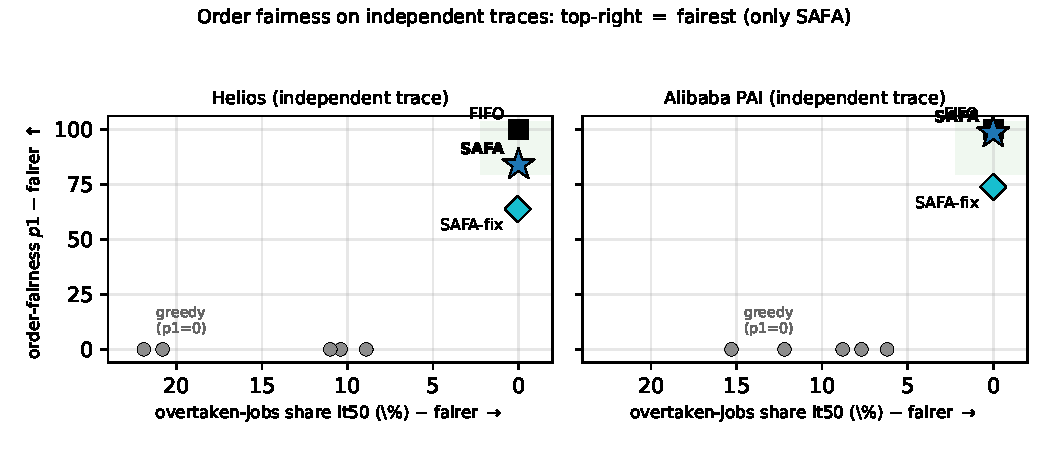
\includegraphics[width=\columnwidth]{Pic/fig_helios.pdf}}
\caption{Helios(Venus) 과부하 이종(동일 모집단 62,069작업): \texttt{lt50\%}(추월 비율, 적을수록 좌측) 대 평균 순서 공정성(높을수록 상단). 마커 구획은 그림 \ref{fig:tradeoff}과 동일(검정=기준선, 회색=어드미션 정책, 청색=SAFA, 삼각=FGD). 본문 \S\ref{eval:robust:trace}.}
\label{fig:helios}
\end{figure}

\begin{table}[htb!]
\centering
\caption{사내 K8S 실측 트레이스(368작업) 독립 일반화 --- 부하점별 하위 1\% 순서 공정성 $p1$. FIFO가 100 미만인 것은 타임스탬프 동률 도착의 tie-break이 도착순을 완전 정의하지 못하는 소표본 효과다.}
\label{tab:inhouse}
\footnotesize
\begin{tabular}{@{}l@{\hspace{1.0em}}rrr@{\hspace{1.2em}}rrr@{}}
\toprule
 & \multicolumn{3}{c}{\textbf{단일 $p1$}} & \multicolumn{3}{c}{\textbf{이종 $p1$}} \\
\cmidrule(lr){2-4}\cmidrule(lr){5-7}
\textbf{정책} & 8 & 16 & 32 & 8 & 16 & 32 \\
\midrule
FIFO          & 99.5 & 96.8 & 98.2 & 99.5 & 96.8 & 97.6 \\
SJF           & 0    & 0    & 86.6 & 0    & 0    & 57.7 \\
LAS           & 0    & 0    & 86.8 & 0    & 0    & 62.2 \\
Kueue         & 0    & 0    & 86.8 & 0    & 0    & 62.2 \\
EASY          & 0    & 0    & 97.5 & 0    & 0    & 93.2 \\
Themis        & 0    & 0    & 81.5 & 0    & 0    & 5.6  \\
FGD           & 0    & 0    & 86.8 & 0    & 0    & 62.2 \\
SAFA(고정 $\alpha$) & 88.8 & 81.7 & 98.1 & 88.8 & 77.8 & 91.3 \\
\textbf{SAFA} & \textbf{98.1} & \textbf{90.0} & 98.1 & \textbf{98.1} & \textbf{92.1} & \textbf{93.4} \\
Lucid         & 0    & 0    & 83.9 & 0    & 0    & 0    \\
\bottomrule
\end{tabular}
\end{table}

\paragraph{세 번째 독립 트레이스: Alibaba PAI}
일반화를 한층 더 확인하기 위해 \textbf{Alibaba PAI GPU 트레이스}\cite{weng2022mlaas}(``MLaaS in the Wild'', NSDI'22; cluster-trace-gpu-v2020) --- Philly·Helios와 독립인 세 번째 대규모 프로덕션 로그 --- 를 재생했다(표 \ref{tab:alibaba}). 완료(\textit{Terminated}) 작업·유효 시각으로 거르고 Alibaba의 백분율 분수-GPU 표기를 정수로 변환($\mathit{plan\_gpu}{\ge}100{\Rightarrow}\mathrm{round}(/100)$, 분수 단독은 1로 올림, gang $={}\mathit{inst\_num}{\times}$per-GPU)한 뒤 seed-42 무작위 16.4\% 서브샘플로 120,105작업(Philly·Helios급)을 얻었다. 동일 256/512/1024 규모에서 부하배수가 3.69$\times$/1.84$\times$/0.92$\times$로 Philly와 일치한다. Philly·Helios와 \textit{동일 메커니즘}이 재현된다 --- 비차단 정책들(LAS·Kueue·FGD·EASY)은 중앙 대기를 낮추는 대가로 작업의 7.7--15.3\%를 추월에 빠뜨려(\texttt{lt50\%}, $p1{=}0$) 큰 작업을 영구히 뒤로 미는 반면, 무튜닝 SAFA는 \textbf{\texttt{lt50\%} 0.0\%($p1{=}98.4$)}로 추월을 제거하며 고정 $\alpha$(0.0\%, 73.8)보다도 p1이 25점 높다. (방법 정정을 여기에도 공개한다: Venus와 동일하게 용량(256 GPU) 초과 요청 26건이 blocking 정책을 조기 차단하는 모집단 결함이 있어, $\le$256 필터 후 동일 모집단 120,079로 blocking 계열을 재실행했다 --- 정정 전 고정 $\alpha$의 ``붕괴''(7.9)는 이 결함의 산물이었다.) 특히 Alibaba는 짧은-꼬리 작업이 많아 그리디의 추월이 Philly보다 \textit{오히려 크고}(EASY 15.3\% 대 13.8\%), worst-1\% $p1$ 우위($98.4$ 대 비차단 0)도 직접 드러난다.

\begin{table}[htb!]
\centering
\caption{Alibaba PAI(NSDI'22, 120k 작업) 과부하 이종(256 GPU, 3.69$\times$), 10정책(동률 행 병합). \texttt{lt50\%}=추월 순서 불공정, $p1$=worst-1\% 순서 공정성, $q_{p50}$=중앙 대기. 무튜닝 SAFA가 \texttt{lt50\%} 0.0·$p1{=}98.4$로 추월 불공정을 제거. 전 정책 \textbf{동일 모집단} 120,079작업(용량 초과 26건 제거 --- Helios와 같은 blocking 차단 결함을 발견·정정; Lucid도 전수 재실행; 테넌트 무정보라 Kueue는 단일-VC 퇴화).}
\label{tab:alibaba}
\footnotesize
\begin{tabular}{@{}l@{\hspace{1.2em}}rrr@{}}
\toprule
\textbf{정책} & \textbf{lt50\%}$\downarrow$ & $p1\uparrow$ & $q_{p50}$ (s) \\
\midrule
\textbf{SAFA} & \textbf{0.0} & \textbf{98.4} & 18.8M \\
FIFO          & 0.0  & 100.0 & 19.2M \\
SAFA(고정 $\alpha$) & 0.0 & 73.8  & 18.6M \\
\midrule
Themis        & 7.7  & 0 & 298 \\
Lucid         & 6.2  & 0 & 0 \\
SJF           & 8.8  & 0 & 96 \\
LAS/Kueue/FGD & 12.2 & 0 & 23K \\
EASY          & 15.3 & 0 & 405K \\
\bottomrule
\end{tabular}
\end{table}

\paragraph{세 트레이스 종합}
Philly·Helios·Alibaba 세 독립 대규모 트레이스에서 같은 결론이 반복된다(표 \ref{tab:trace3}): 과부하 이종에서 정보-우위 그리디는 추월 불공정(\texttt{lt50\%})이 두 자릿수이고, 무튜닝 SAFA는 어느 트레이스에서도 \texttt{lt50\%}를 비차단 정책 중 최저(0.0--0.08\%; 기준선 FIFO는 정의상 0)로 억제하며, worst-1\% $p1$에서도 고정 $\alpha$를 13--25점 일관 상회한다(이종 과부하 512/80/256에서 50.5 대 37.3, 83.9 대 63.7, 98.4 대 73.8 --- 동일 코드; 표의 Philly 열은 256 구성). worst-1\% $p1$은 세 트레이스 모두에서 SAFA 우위가 일관된다(50.5--98.4 대 비차단 0).

\begin{table}[htb!]
\centering
\caption{세 독립 트레이스 종합 --- 과부하 이종 한 점씩(Philly 256/3.6$\times$, Helios 80/과부하, Alibaba 256/3.69$\times$)의 추월 순서 불공정 \texttt{lt50\%}(낮을수록 공정). 무튜닝 SAFA가 세 트레이스 모두에서 비차단 정책 중 최저($\approx$0; FIFO는 정의상 0).}
\label{tab:trace3}
\footnotesize
\begin{tabular}{@{}l@{\hspace{1.4em}}rrr@{}}
\toprule
\textbf{정책 (\texttt{lt50\%})} & Philly & Helios & Alibaba \\
\midrule
FIFO          & 0.0  & 0.0  & 0.0 \\
LAS/Kueue/FGD & 8--11 & 20.8 & 12.2 \\
SJF           & 7.4  & 10.4 & 8.8  \\
EASY          & 13.8 & 21.9 & 15.3 \\
Themis        & 7.9  & 11.0 & 7.7 \\
Lucid         & 3.4  & 8.9  & 6.2 \\
SAFA(고정 $\alpha$) & 4.9  & 0.05 & 0.0 \\
\textbf{SAFA} & \textbf{0.08} & \textbf{0.0} & \textbf{0.0} \\
\bottomrule
\end{tabular}
\end{table}

\subsubsection{시뮬레이터 충실도 검증}\label{eval:robust:fidelity}
모든 결과가 자체 이산 사건 시뮬레이터에 의존하므로, 엔진이 큐잉 동역학을 정확히 계산하는지 \textit{해석해를 손계산할 수 있는} 세 가지 toy 사례와 대조했다: (i) 포화 D/D/1 FIFO 큐(잡 $k$의 큐 지연 $=k(S-I)$), (ii) 다중 GPU 노드의 gang 동시 스케줄링, (iii) 수명주기 오버헤드 회계(place\,$=$\,arrival\,$+$\,sched\_lat\,$+$\,startup, finish\,$=$\,place\,$+S+$\,teardown). 엔진은 세 사례의 손계산 큐 지연·완료 시각을 \textbf{모두 부동소수점 정밀도 내(최대 절대오차 $0.0$)}로 재현했다 --- 즉 본 평가의 ``실측의 제한된 범위''(\S\ref{eval:threats})는 절대값의 운영적 대표성에 대한 한계이지 큐잉 동역학 계산의 정확성 문제는 아니다.

\subsubsection{배치 무관성: 어떤 배치 정책 위에서도}\label{eval:robust:placement}
SAFA의 핵심 정체성은 \textit{배치-전 어드미션 순서 계층} --- ``어떤 작업을 먼저''만 결정하고 ``어디에''(배치)는 다음 단계에 맡긴다 --- 이므로, 그 이점이 \textit{특정 배치}에 의존하지 않아야 한다. 지금까지 결과는 most-allocated 배치 위에서 얻었다. 이를 검증하기 위해 동일 SAFA 큐 전처리를 \textbf{4개의 서로 다른 코어 배치}(most-allocated, compact, round-robin, MCTS) 위에 얹어 재실험했다(표 \ref{tab:placement}, 그림 \ref{fig:placement}). round-robin은 빈자리가 많은 노드를 우선하는 분산 배치, MCTS는 후보 노드마다 롤아웃으로 달성 할당률을 추정해 고르는 탐색 배치로, C++ 원본 스케줄러를 포팅했다. 결과는 명확하다: \textbf{SAFA의 $p1$이 4개 배치 전부$\times$과부하 4구성(단일·이종 256/512)에서 50--70으로 유지}된다(256 단일 추가 측정 포함). 베이스라인과의 대비는 구성을 가른다 --- 이종에서는 SJF·LAS가 전 배치에서 0으로 붕괴하는 반면, 512 단일에서는 \S\ref{eval:main}에서 본 대로 SJF가 회복해(64.1) 네 배치의 SAFA(53.1--62.1)를 모두 넘고, 256 단일에서는 0이다 --- 즉 배치 불변인 것은 \textit{SAFA 자신의 안정성}이고, 정책 간 순위는 구성(경합 깊이)이 정한다. 배치가 절대 큐 지연에 주는 영향은 작고(SAFA의 $q_{p50}$ 변동 5--15\%, FIFO·SJF는 $\le$1.5\%) 순위를 바꾸지 않는다. 직교의 \textit{결합 방향}도 직접 검증했다: SAFA 어드미션 순서를 단편화 인지 배치 FGD 위에 그대로 얹으면(SAFA$\oplus$FGD) 512 단일/이종에서 (53.5, 621K)/(50.1, 1.79M)으로 SAFA 단독과 사실상 동일하다 --- 과포화라 배치 이득 자체는 없지만, 두 층위가 간섭 없이 결합됨이 측정으로 확인된다(collocation 실행 모델을 가진 Lucid와의 결합은 엔진 통합이 필요한 향후 과제). 즉 SAFA의 기여는 배치 휴리스틱과 \textit{직교}하며, 어떤 배치 정책 위에서도 작동하는 어드미션 순서 계층이라는 주장이 실증된다. (MCTS 배치 비용은 most-allocated 대비 1.0--1.9$\times$, 111k 작업에서 최대 87초로 전수 트레이스에서도 현실적이었다. most-allocated 결과는 표 \ref{tab:sim-single}·\ref{tab:sim}의 해당 셀과 정확히 일치해 배치 주입이 회귀를 일으키지 않음을 확인했다.)

\begin{table}[htb!]
\centering
\caption{배치 무관성 --- 4개 코어 배치별 SAFA 하위 1\% 순서 공정성 $p1$(그림 \ref{fig:placement}).}
\label{tab:placement}
\footnotesize
\begin{tabular}{@{}l@{\hspace{1.2em}}rrrr@{}}
\toprule
\textbf{코어 배치} & 256 단일 & 256 이종 & 512 단일 & 512 이종 \\
\midrule
most-allocated & 54.3 & 54.4 & 53.1 & 50.5 \\
compact        & 55.6 & 54.0 & 54.2 & 52.2 \\
round-robin    & \textbf{69.7} & \textbf{59.5} & \textbf{62.1} & \textbf{53.7} \\
MCTS           & 56.6 & 53.4 & 55.0 & 50.6 \\
\midrule
\textit{(참고) SJF} & 0 & 0 & 64.1 & 0 \\
\textit{(참고) LAS} & 0 & 0 & 30.9 & 0 \\
\bottomrule
\end{tabular}
\end{table}

\begin{figure}[htb!]
\centerline{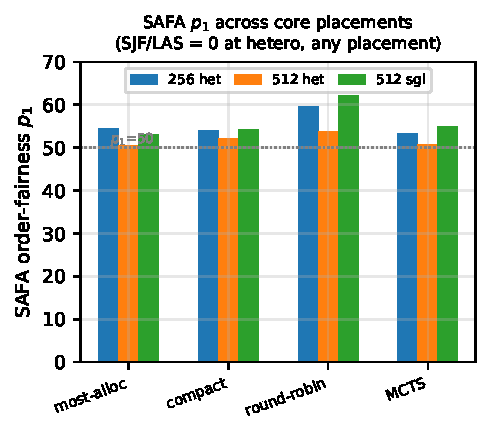
\includegraphics[width=\columnwidth]{Pic/fig_placement.pdf}}
\caption{4개 코어 배치별 SAFA 하위 1\% 순서 공정성(무튜닝). 본문 \S\ref{eval:robust:placement}.}
\label{fig:placement}
\end{figure}

\subsection{실 클러스터 실측 검증(B200)}\label{eval:b200}
위 결과는 모두 시뮬레이션이다. 큐-축 비교 정책을 NVIDIA B200$\times$8 단일 노드 쿠버네티스(v1.31, kind 기반 --- 프로덕션 컨트롤플레인과 바인딩 경로가 다를 수 있음)에서 실측해 시뮬 경향을 실 클러스터에서 교차 검증한다 --- \S\ref{eval:overhead}의 수명주기 오버헤드를 이미 이 클러스터에서 계측했으며, 동일 하니스로 큐잉 지연·JCT를 실측한다(표 \ref{tab:b200}). (배치 축·합성계수 민감도는 단일 노드에 정의되지 않거나 실 클러스터에 대응 개념이 없어 시뮬 전담이며, 노드 간 배치·collocation은 다중 노드 합류 시의 향후 과제다.)

Philly에서 추출한 500작업(JCT$\le$2시간 윈도우, heavy-tail duration 보존: 시간압축 후 $p50$ 11초·$p99/p50\approx20\times$ --- 중앙값 작업이 게이트 주기 $\Delta{=}5$초의 2배라 주기 아티팩트가 1차 효과인 짧은-작업 레짐; 시간 단위 작업 레짐의 게이트 거동은 외삽이다)을 \texttt{submit-clamp}로 압축 제출해 실제로 8/8 GPU 포화·대기 큐 47개의 과부하 구간을 형성했다(순서 공정성은 실 wall 제출시각 기준). 컨트롤러의 배포 의미론(wall-clock 나이·주기 $\Delta$ 게이트·greedy 해제)은 시뮬 엔진(도착 카운터·사건 구동)과 다르므로, 실행 전 동일 트레이스의 오프라인 충실 리플레이로 이 의미론을 별도 점검했고 그 예측이 실측과 부합했다(lt50 5.2\%는 일치, $q_{p50}$ 398$\to$423초는 $+6.3\%$) --- 두 의미론이 본 레짐에서 같은 거동으로 수렴함의 직접 근거다. 표 \ref{tab:b200}에서 시뮬의 세 경향이 실 클러스터에서 재현된다: (i) 그리디·비순서 정책(기본 kube-scheduler 49.8\% --- backoff·병렬 바인딩으로 비FIFO, Themis 31.4\%, SJF 30.4\%)이 높은 추월 순서 불공정(\texttt{lt50\%})을 보이고, (ii) 자리 예약·admission 정책(EASY 1.8\%, Kueue 4.4\%)이 추월을 억제해 가장 공정하며, (iii) SAFA는 고정 $\alpha$와 무튜닝(제안) 모두 \texttt{lt50} 5.2\%로 FIFO-gate(6.2\%)·LAS(5.2\%) 수준의 순서 공정성을 유지한다($n{=}500$ 단일 런이라 4--6\% 군 내부의 순위는 이항 신뢰구간 안에서 비결정 --- 군 간 대비(공정군 2--6\% 대 그리디군 30--50\%)로 읽어야 한다). 특히 무튜닝 SAFA(5.2\%, $q_{p50}$ 423초)는 고정 $\alpha$(5.2\%, 424초)와 사실상 구별되지 않아, 노브 없이 고정 $\alpha$ 수준 공정성을 달성한다는 \S\ref{SAFA}의 무튜닝(zero-knob) 주장을 실 클러스터에서 확인한다. 표에서 게이트 계열의 평균 할당률이 기본 kube-scheduler보다 7--11\%p 낮은 점도 숨기지 않는다(EASY 11\%p 최대). 한 가지 회계 주의: alloc은 폴링 평균이고 walltime과 적분 창(시작·드레인 경계)이 달라 두 값의 곱은 GPU-시간 보존을 재현하지 않는다 --- 각 수치는 점유 추세와 총 소요로만 읽고 정책 간 곱 비교는 하지 말 것 --- 주기 $\Delta{=}5$초의 어드미션 지연이 짧은 작업 사이에 유휴 갭을 만든 게이트 아키텍처의 비용이다. 다만 이 갭은 처리량 손실로 이어지지 않았고(게이트 계열 walltime 51--54분 $<$ 기본 68분), $\Delta$ 축소나 이벤트-구동 게이트 해제로 줄일 수 있는 구현 비용이지 알고리즘 비용이 아니다. 같은 표의 FIFO(gate) lt50\% 6.2\%는 또 하나의 정직한 관측이다 --- 게이트 해제 \textit{순서}가 kube-scheduler의 내부 큐(activeQ/backoff)와 병렬 바인딩을 통과하며 완전히 보존되지는 않아, 게이트는 순서의 \textit{강한 편향}이지 보장이 아니다. SAFA(5.2\%)가 FIFO(gate)와 같은 수준인 것은 이 바닥 누설 위에서 측정된 결과다.

다만 이 단일 노드·균일 도착 구간이 검증하는 범위는 한정적임을 명시한다. \texttt{submit-clamp}로 도착을 균일화하면 대기 큐 안에서 작업의 나이 순서가 도착 순서와 일치하므로, SAFA의 나이 승급(\S\ref{SAFA})은 이 구간에서 FIFO(자원 가중 포함)로 퇴화한다. 따라서 단일 노드 실측이 확인하는 것은 (a) SAFA의 큐 재정렬 축이 실 K8s에서 \textit{안전}하게 동작하며 그리디류의 추월 불공정을 일으키지 않는다는 점과, (b) 무튜닝 계수가 고정 $\alpha$ 수준으로 수렴한다는 점이다. 나이 승급이 \textit{또래 대비 굶주린 큰 작업을 선별 승급}하는 고유 가치는 도착 버스트와 다중 노드 단편화가 동시에 작용할 때 드러나며, 그 축은 본 평가의 시뮬레이션(256--1024 GPU, 트레이스 버스트)이 담당한다.

\begin{table}[htb!]
\centering
\caption{B200$\times$8 단일 노드 실 클러스터 실측(500작업, 과부하). 주 지표 \texttt{lt50\%}(추월 순서 불공정 비율, 낮을수록 공정)·평균 순서 공정성. 본문 \S\ref{eval:b200}.}
\label{tab:b200}
\footnotesize
\begin{tabular}{@{}l@{\hspace{1.2em}}rrrr@{}}
\toprule
정책 & \texttt{lt50\%}$\downarrow$ & fair평균 & $q_{p50}$(s) & alloc \\
\midrule
기본 kube-sched(비FIFO) & 49.8 & 56.3 & 857 & 91\% \\
FIFO (gate) & 6.2 & 93.8 & 422 & 84\% \\
SJF & 30.4 & 71.9 & 15 & 82\% \\
LAS & 5.2 & 94.5 & 424 & 84\% \\
Kueue & 4.4 & 95.6 & 449 & 82\% \\
EASY & 1.8 & 96.6 & 1138 & 80\% \\
Themis & 31.4 & 70.6 & 76 & 84\% \\
\midrule
SAFA (고정 $\alpha$) & 5.2 & 94.4 & 424 & 83\% \\
\textbf{SAFA (제안)} & \textbf{5.2} & \textbf{94.6} & 423 & 83\% \\
\bottomrule
\end{tabular}
\end{table}

\subsection{타당성 위협(Threats to validity)}\label{eval:threats}
강건성 검증(\S\ref{eval:robust})에도 불구하고 본 평가는 다음 한계를 가지므로, 결과는 절대값보다 \textit{경향}으로 해석해야 한다. (1) \textbf{실측의 제한된 범위}: 주 평가는 시뮬레이터에 의존하며, 큐-축 정책을 B200$\times$8 \textit{단일 노드} 실 클러스터에서 교차 검증했으나(\S\ref{eval:b200}) 이는 단일 노드·균일 도착 구간에 한정된다(엔진의 \textit{계산} 충실도는 별도로 \S\ref{eval:robust:fidelity}에서 확인). 다중 노드 단편화·버스트 도착의 end-to-end 실측은 향후 과제다. 부하 축에서도 준임계와 지속 과포화 사이의 \textit{반복 버스트-드레인}(어드미션 컨트롤이 있는 운영 동작점) 레짐은 미평가이며, 도착-카운터 나이는 드레인 구간마다 승급 압력이 동결되므로 그 레짐의 거동은 별도 검증이 필요하다. (2) \textbf{모델 단순화}: 네트워크 대역폭, 작업 간 간섭, 자원 경합을 모델링하지 않았고, 작업 실행시간을 ``명목 실행시간\,$\times$\,타입 속도계수\,$+$\,고정 오버헤드''로 단순화했다 --- 이는 collocation·간섭에 민감한 정책(특히 Lucid)의 거동을 단순화할 수 있다. (3) \textbf{워크로드 대표성}: 주 평가는 단일 트레이스(Philly)에 기반하므로 대표성이 제한되며, \S\ref{eval:robust:trace}에서 두 대규모 독립 트레이스(Helios·Alibaba)와 사내 실측으로 보강하나 각각도 유한한 표본이다. 또한 수명 주기 오버헤드는 B200$\times$8 단일 노드에서 \textit{실측}했으나(\S\ref{eval:overhead}) 노드 간 이주 네트워크 비용은 반영하지 못했고, 타입 속도계수는 처리량 비(比)에 근거한 모델값이다. 타입-인지 배치의 영향도 점검했다 --- 속도계수 기반 빠른-타입-우선 배치를 코어로 바꿔도 512 이종에서 FIFO·SJF·SAFA의 지표가 변하지 않아(SAFA 50.5/1.76M 동일), 과포화에서는 이종 우위가 배치 선택의 인공물이 아니다. 반면 \textit{작업이 타입을 고정}하는 구속 환경(타입별 풀 분리)에서는 현재의 타입-비인지 $R$이 승급 신호를 잃어 SAFA가 FIFO와 동치로 퇴화함을 확인했다 --- 타입 구속 클러스터에는 $R$의 타입별 확장이 선결이다(향후 과제)(빈 슬롯 희소로 배치 자유도가 소진되는 \S\ref{eval:main}의 FGD 관찰과 일관). 아울러 본 평가의 gang은 노드 한 대에 들어가는 $\le$8-GPU \textit{정수} 요청이며 $R$ 테이블도 노드당 8 슬롯 기준 단일 자원으로 정의된다 --- CPU·메모리·NIC가 함께 묶이는 다차원 요청과 MIG·time-slicing의 분수 GPU에는 $R$의 일반화가 필요하다. 또한 --- 수십$\sim$수백 GPU 멀티노드 gang(LLM 사전학습)에는 $R$의 정의를 노드 묶음 단위로 확장해야 하며, 그 영역에서의 검증은 다중 노드 실측과 함께 향후 과제다. (4) \textbf{탄력 SOTA 제외}: 더 무거운 정보를 요구하는 탄력 스케줄러(Sia·Arena·RLTune\cite{arena2026,rltune2025} 류)는 결정 변수를 고정 요청 트레이스로 정의할 수 없어 동일 엔진에서 제외했다 --- Sia의 합성 프로파일 포팅이 원 논문·후속 비평과 수치가 어긋남을 직접 확인한 것이 그 근거다(\S\ref{baseline-rationale}). 이는 ``SAFA가 모든 스케줄러보다 낫다''가 아니라 ``부차 정보 없이 동작하는 배치-전 어드미션 순서 계층''이라는 한정으로 이어진다. (5) \textbf{주·부차 지표의 편향과 순환 가능성}: slowdown 계열 지표(BSLD, 임계 $\tau{=}10$초의 bounded slowdown\cite{feitelson1998metrics})는 도착 \textit{순서}를 보지 않고 서비스 시간으로 정규화하여 짧은 작업 우선 정책에 본질적으로 유리하므로 부차 지표로만 보고한다. 역으로 주 지표인 도착 순서 공정성(p1)은 도착순 보존을 정의로 삼아 도착순 보존형 정책(SAFA 포함)에 구조적으로 유리할 수 있다 --- 이 순환 가능성은 SAFA가 최적화하지 않은 독립 분배 지표(대기 Gini·p99/p50 비, 표 \ref{tab:indep})와 임계 스윕으로 교차 점검했고 \texttt{lt25/50}에서 대비가 유지됨을 확인했으나(\texttt{lt75}에선 일부 순위 역전 --- \S\ref{eval:main}), 지표 선택이 결론의 프레임을 정한다는 한계 자체는 남는다. 종합하면 본 평가의 결론은 정책 간 절대 순위가 아니라, 이질성·부하가 깊어질 때 나타나는 \textit{공정성 붕괴 대 유지의 질적 경향}에 무게를 둔다.

\subsection{Lifecycle overhead model}\label{eval:overhead}
이산 사건 시뮬레이터는 작업당 고정 오버헤드(스케줄링·기동·종료)를 주입하여 충실도를 높인다. 이 보정값은 가정이 아니라 \textit{실측}이다: 우리는 NVIDIA B200$\times$8 단일 노드 쿠버네티스(v1.31, kind) 클러스터에서 47개 작업을 4개 시나리오(단독 순차, 동시 8, 동시 24, 대형 gang)로 실행해 작업 수명 주기의 각 구간을 계측했다(이미지 캐시 상태 기준 --- 콜드 풀의 수십 GB CUDA 이미지는 기동을 분 단위로 늘릴 수 있어 별도 항으로 보아야 한다). 측정값에 맞춰 고정 오버헤드를 작업당 4.5--6.5초 --- 스케줄링 지연 0.5초, 컨테이너 기동 1.5--3.5초, 종료(teardown$\to$complete) 2.5초 --- 로 설정한다. 기동 비용은 단독 배치(이미지 캐시 상태에서 p50 1초, p90 2초 $\to$ 1.5초)와 혼잡 배치(동시 2개 이상, p50 3초·p90 4초 $\to$ 3.5초)를 구분하여, 공유 노드에 여러 gang이 동시에 올라올 때의 컨테이너 초기화 경합을 반영한다. 중요한 점은 동시 24 시나리오에서 관측된 17--36초의 스케줄링 지연은 \textit{오버헤드가 아니라 용량 대기(큐잉)}이며, 시뮬레이터가 정책 로직으로 직접 산출하므로 고정 오버헤드에 포함하지 않는다(이중 계상 방지) --- 주입하는 것은 스케줄링 지연$+$기동$+$종료(작업당 4.5--6.5초)이며, 용량 대기(큐잉)는 정책 로직이 산출한다 --- 충실도 검증(\S\ref{eval:robust:fidelity})의 회계도 이 명세(place $=$ arrival $+$ sched\_lat $+$ startup) 기준이다.

\textbf{B200 기준 오버헤드 고려.} 본 평가의 기준(reference) 가속기는 NVIDIA B200이다. 작업의 명목 실행시간은 배치된 GPU 타입의 속도계수로 스케일하며($\textsc{speed}$: B200 $=1.0$ 기준, H100 $\approx1.4$, A100 $\approx2.0$, A30 $\approx2.8$), gang이 타입을 혼합하면 가장 느린 타입을 기준으로 한다(동기 학습의 straggler 제약). 따라서 단일 클러스터(전부 B200)에서는 옛 트레이스의 실측 실행시간이 그대로 쓰이고, 이종 클러스터에서는 느린 타입에 놓인 작업이 비례적으로 길어진다 --- 이것이 이종 환경에서 베이스라인의 HOL 블로킹이 더 심해지는 한 원인이다. 한편 위 4.5--6.5초의 수명 주기 오버헤드는 위에서 기술한 B200$\times$8 클러스터 실측값으로, 일(day) 단위에 이르는 작업 실행시간에 비하면 작지만, 과부하에서 누적되는 짧은 작업의 큐잉 지연에는 유의미하게 기여한다. \S\ref{SAFA}의 민감도 분석이 보였듯 최종 결과는 이 보정값의 넓은 범위에 둔감하다. 본 실측은 단일 노드이므로 노드 간 이주 네트워크 비용은 0으로 두며, 이는 H100 노드 합류 시 추가 계측할 향후 과제다.

\FloatBarrier

\section{Conclusions and Future Works}\label{conclu}

본 연구는 GPU 서버 풀에서 HOL 블로킹으로 인한 기아를 해소하기 위해, 스케줄링의 첫 단계(어드미션 순서)만을 담당하는 계층 SAFA를 제안했다. 평가는 두 시뮬레이터와 실측이 역할을 나누어, 나이 가중 계수 $\alpha$의 동기는 분포별 합성 트레이스 위의 C++ 이산 시간 시뮬레이터로 분석하고, 동일 엔진 비교(기준선 FIFO·어드미션 순서 정책 6종·배치 축 참고)는 Philly 111k 작업 규모의 이산 사건 시뮬레이터(256--1024 GPU, 단일·이종)로 수행했으며, 큐-축 정책들은 NVIDIA B200$\times$8 단일 노드 쿠버네티스에서 실측해 시뮬 경향을 교차 검증했다. 기아를 다루는 종래 기법들이 실행시간 추정·성능 프로파일·솔버 같은 부차 정보를 요구하는 것과 달리, SAFA는 코어 스케줄링 정책을 그대로 유지한 채 \textit{큐에서 관측되는 정보만으로}(대기 시간·자원 요구량·상대 나이) 큐 선두의 HOL 블로킹을 해소하여 다양한 스케줄러 위에서 동작한다.

무튜닝 SAFA는 빠른 정책들의 하위 1\% 순서 공정성이 0으로 붕괴하는 과부하 이종(256/512)에서 이를 50--54로, 임계(이종 1024)에서 76.5로 유지하면서 중앙값 대기를 FIFO 대비 50--61\% 단축하여(Philly 주 평가; 독립 트레이스에서 효율 이득은 2--15\%로 트레이스 의존, 공정성 우위는 유지), 공정성을 포기하지 않고 빨라졌다. 단일·저경합에서는 Lucid 같은 collocation 정책이 더 빠르고 공정할 수 있으나, 이질성·부하가 깊어질수록 다른 빠른 정책들이 순서 공정성 붕괴를 --- 크기-선별 정책은 큰 작업의 최악 대기 폭증이라는 실제 기아까지 --- 겪는 반면 SAFA는 큐 정보만으로 두 축을 함께 억제했고, 두 독립 대규모 트레이스(Helios·Alibaba)에서도 추월로 순서 공정성을 잃는 작업 비율을 0.1\% 미만으로 억제했다(비차단 정책 6--22\%). 즉 SAFA는 별도 프로파일이나 부차 정보 없이 큐 관측 정보만으로 ``어떤 작업을 먼저''를 결정하는 배치-전 어드미션 순서 계층이며, 배치 정책은 손대지 않는다.

고정 계수 SAFA(고정 $\alpha$)는 최적 계수를 사후(posterior) 반복 탐색으로 찾아야 했고, 해당 목적함수 기준 최적 $\alpha$가 워크로드마다 7배 달라지는 한계가 있었다. 본 연구의 핵심 진전은 이 한계를 무튜닝 SAFA로 해소한 것이다 --- 계수를 사전에 계산해 두는 대신, 관측 가능한 큐 통계(상대 나이)로부터 나이 가중 계수를 무튜닝으로 적응시켜작업 실행 시간(duration) 추정 없이 워크로드 변화에 적응한다.

다만 SAFA는 큐 순서만을 조정하므로, 백로그가 얕은 일부 상황에서는 기아 작업을 상위로 승급시켜도 작은 작업에 자리를 추월당할 수 있다. 이는 향후 연구에서 감지(부하·나이 기반 기아 압력)와 자원 예약(EASY식 자리 잠금, 단 duration 추정 불요)을 결합하여 해소할 계획이다 --- 다만 \textit{예약}(자리 잠금)과 \textit{재정렬}(나이 승급)은 같은 큐에서 충돌할 수 있으므로, 그 상호작용을 분석해 두 메커니즘을 정합시키는 것이 결합의 선결 과제다. 또한 본 평가는 GPU 갱 트레이스(Philly·사내 K8S)에 한정되므로, 표준 워크로드 포맷(SWF) 기반 고전 병렬 작업 트레이스로 평가를 확장해 고전 HPC 배치 스케줄링 문헌과의 가교를 놓는 것도 향후 과제다. 그 밖의 가장 중요한 향후 과제는 \textit{다중 노드(2노드 이상)} 실 클러스터 실측으로, 다음이 한 묶음으로 열린다: (i) 노드 간 단편화가 실재하는 레짐에서 SAFA의 효율 우위 실측(단일 노드에는 그 레짐 자체가 없다 --- 본 버스트 리플레이에서도 단일 노드의 승급 효율 이득은 미미했다), (ii) 멀티노드 gang의 부분 바인딩·원자성 검증, (iii) 노드 간 이주·네트워크 비용 계측, (iv) Kueue-suspend 결합의 per-VC 정량화. 단일 노드에서 가능한 검증 --- blocking-aware 규율·도착-순번 나이의 버스트 거동 --- 은 본 개정에서 참조 구현과 리플레이로 닫았다(\S\ref{SAFA:k8s}).

\FloatBarrier
\section*{Acknowledgment}
저자들은 본 연구에 대해 어떠한 기관의 재정 지원도 받지 않았다.

\textbf{생성형 AI 활용 고지.} IEEE의 권고에 따라, 본 논문 준비 과정에서 저자들은 생성형 AI 도구를 보조적으로 활용하였음을 고지한다. AI는 문장 다듬기·언어 교정, 그림 생성 및 실험 재현용 스크립트 작성, 결과 정리 보조에 한해 사용되었으며, 연구의 착상·알고리즘 설계·실험 수행 및 해석은 저자들이 직접 수행하였다. 저자들은 AI 도구 사용 후 모든 내용을 검토·수정하였고, 출판물의 내용에 대한 전적인 책임은 저자들에게 있다.

%%===========================================================================================%%
%% If you are submitting to one of the Nature Portfolio journals, using the eJP submission   %%
%% system, please include the references within the manuscript file itself. You may do this  %%
%% by copying the reference list from your .bbl file, paste it into the main manuscript .tex %%
%% file, and delete the associated \verb+\bibliography+ commands.                            %%
%%===========================================================================================%%

\bibliographystyle{IEEEtran}
\bibliography{sn-bibliography}
%% if required, the content of .bbl file can be included here once bbl is generated
%%\input sn-article.bbl
\end{document}

